% Arquivo LaTeX de exemplo de dissertação/tese a ser apresentada à CPG do IME-USP
%
% Criação: Jesús P. Mena-Chalco
% Revisão: Fabio Kon e Paulo Feofiloff
% Adaptação para UTF8, biblatex e outras melhorias: Nelson Lago
%
% Except where otherwise indicated, these files are distributed under
% the MIT Licence. The example text, which includes the tutorial and
% examples as well as the explanatory comments in the source, are
% available under the Creative Commons Attribution International
% Licence, v4.0 (CC-BY 4.0) - https://creativecommons.org/licenses/by/4.0/


%%%%%%%%%%%%%%%%%%%%%%%%%%%%%%%%%%%%%%%%%%%%%%%%%%%%%%%%%%%%%%%%%%%%%%%%%%%%%%%%
%%%%%%%%%%%%%%%%%%%%%%%%%%%%%%% PREÂMBULO LaTeX %%%%%%%%%%%%%%%%%%%%%%%%%%%%%%%%
%%%%%%%%%%%%%%%%%%%%%%%%%%%%%%%%%%%%%%%%%%%%%%%%%%%%%%%%%%%%%%%%%%%%%%%%%%%%%%%%

% A opção twoside (frente-e-verso) significa que a aparência das páginas pares
% e ímpares pode ser diferente. Por exemplo, as margens podem ser diferentes ou
% os números de página podem aparecer à direita ou à esquerda alternadamente.
% Mas nada impede que você crie um documento "só frente" e, ao imprimir, faça
% a impressão frente-e-verso.
%
% Aqui também definimos a língua padrão do documento
% (a última da lista) e línguas adicionais.
%\documentclass[12pt,twoside,brazilian,english]{book}
\documentclass[12pt,twoside,english,brazilian]{book}

% Ao invés de definir o tamanho das margens, vamos definir os tamanhos do
% texto, do cabeçalho e do rodapé, e deixamos a package geometry calcular
% o tamanho das margens em função do tamanho do papel. Assim, obtemos o
% mesmo resultado impresso, mas com margens diferentes, se o tamanho do
% papel for diferente.
\usepackage[a4paper]{geometry}

% Escrita de teoremas e lemas
\usepackage{amsthm}
\newtheorem{theorem}{Teorema}[section]
\newtheorem{lemma}[theorem]{Lema}

\geometry{
  textwidth=152mm,
  hmarginratio=12:17, % 24:34 -> com papel A4, 24mm + 152mm + 34mm = 210mm
  textheight=237mm,
  vmarginratio=8:7, % 32:28 -> com papel A4, 32mm + 237mm + 28mm = 297mm
  headsep=11mm, % distância entre a base do cabeçalho e o texto
  headheight=21mm, % qualquer medida grande o suficiente, p.ex., top - headsep
  footskip=10mm,
  marginpar=20mm,
  marginparsep=5mm,
}

% Vários pacotes e opções de configuração genéricos; para personalizar o
% resultado, modifique estes arquivos.
%%%%%%%%%%%%%%%%%%%%%%%%%%%%%%%%%%%%%%%%%%%%%%%%%%%%%%%%%%%%%%%%%%%%%%%%%%%%%%%%
%%%%%%%%%%%%%%%%%%%%%%% CONFIGURAÇÕES E PACOTES BÁSICOS %%%%%%%%%%%%%%%%%%%%%%%%
%%%%%%%%%%%%%%%%%%%%%%%%%%%%%%%%%%%%%%%%%%%%%%%%%%%%%%%%%%%%%%%%%%%%%%%%%%%%%%%%

% Vários comandos auxiliares para o desenvolvimento de packages e classes;
% aqui, usamos em alguns comandos de formatação e condicionais.
\usepackage{etoolbox}
\usepackage{xstring}
\usepackage{expl3}
\usepackage{xparse}
\usepackage{letltxmacro}
\usepackage{regexpatch}

% O projeto LaTeX3 renomeou algumas macros em 2019-03-05 e removeu
% a compatibilidade com os nomes antigos em 2020-07-17 a partir de
% 2021-01-01 (veja o arquivo l3deprecation.dtx e o changelog em
% https://github.com/latex3/latex3/blob/main/l3kernel/CHANGELOG.md).
% Isso afetou a package regexpatch: versões antigas da package não
% funcionam com versões novas de LaTeX e vice-versa. Infelizmente,
% ubuntu 21.04 (hirsute) e debian 11 (bullseye) incluem essas versões
% incompatíveis e, portanto, a package regexpatch não funciona nesses
% ambientes. Talvez fosse possível contornar esse problema com a
% package latexrelease, mas isso afetaria muitos outros recursos.
% Ao invés disso, vamos restaurar manualmente a compatibilidade.
% TODO: remover isto após debian bullseye se tornar obsoleta,
%       provavelmente no final de 2024.
\makeatletter
\ExplSyntaxOn

\@ifpackagelater{regexpatch}{2021/03/21}
  {} % Se regexpatch é "nova", expl3 deve ser também; nada a fazer
  {
    % Talvez o correto seja 2021/01/01, mas na prática o resultado é o mesmo
    \@ifpackagelater{expl3}{2020/07/17}
      {
        % As versões são incompatíveis; vamos recuperar as macros preteridas
        \cs_gset:Npn \token_get_prefix_spec:N { \cs_prefix_spec:N }
        \cs_gset:Npn \token_get_arg_spec:N { \cs_argument_spec:N }
        \cs_gset:Npn \token_get_replacement_spec:N { \cs_replacement_spec:N }
      }
      {} % As duas packages são antigas e, portanto, compatíveis entre si
  }
\ExplSyntaxOff
\makeatother

% Algumas packages dependem de xpatch e tentam carregá-la, causando conflitos
% com regexpatch. Como regexpatch oferece todos os recursos de xpatch (ela
% é uma versão estendida de xpatch, mas ainda considerada experimental), vamos
% fazê-las acreditar que xpatch já foi carregada.
\expandafter\xdef\csname ver@xpatch.sty\endcsname{2012/10/02}

% Arithmetic expressions in \set{length,counter} & \addto{length,counter};
% commands \widthof, \heightof, \depthof, \totalheightof, \settototalheight
\usepackage{calc}

% Sempre que possível, é melhor usar os recursos de etoolbox ao invés de
% ifthen; no entanto, várias packages dependem dela.
%\usepackage{ifthen}

% Esta não está em uso mas pode ser útil.
%\usepackage{ltxcmds}

%\usepackage{xfp} % Floating-point calculations

% Esta package permite detectar XeTeX, LuaTeX e pdfTeX, mas pode não estar
% disponível em todas as instalações de TeX.
%\usepackage{iftex}
% Por conta disso, usaremos estas (que não detectam pdfTeX):
\usepackage{ifxetex}
\usepackage{ifluatex}

\newbool{unicodeengine}
\ifboolexpr{bool{xetex} or bool{luatex}}
  {\booltrue{unicodeengine}}
  {\boolfalse{unicodeengine}}

% Detecta se estamos produzindo um arquivo PDF ou DVI (lembrando que tanto
% pdfTeX quanto LuaTeX podem gerar ambos)
\usepackage{ifpdf}

% Algumas packages "padrão" da AMS, que são praticamente obrigatórias.
% Algumas delas devem ser carregadas antes de unicode-math ou das
% definições das fontes do documento.
\usepackage{amssymb}
\usepackage{amsthm}
\usepackage{amsmath}

% "fontenc" é um parâmetro do NFSS (sistema de gestão de fontes do
% LaTeX; consulte "texdoc fntguide" e "texdoc fontenc"). O default
% é OT1, mas ele tem algumas limitações; a mais importante é que,
% com ele, palavras acentuadas não podem ser hifenizadas. Por
% conta disso, quase todos os documentos LaTeX utilizam o fontenc
% T1. A escolha do fontenc tem consequências para as fontes que
% podem ser usadas com NFSS; hoje em dia T1 tem mais opções de
% qualidade, então não se perde nada em usá-lo. A package fontspec
% (para gestão de fontes usando outro mecanismo, compatível apenas
% com lualatex e xelatex) carrega fontenc automaticamente, mas
% usando outra codificação ("TU" e não "T1"). Ainda assim, é útil
% carregar o fontenc T1 (antes de carregar fontspec!) para o caso
% de alguma fonte "antiga" ser utilizada no documento (embora isso
% não seja recomendado: lualatex e xelatex só são capazes de
% hifenizar palavras acentuadas com o fontenc TU).
\usepackage[T1]{fontenc}

\ifunicodeengine
  % Não é preciso carregar inputenc com LuaTeX e XeTeX, pois
  % com eles utf8 é obrigatório.
  \usepackage{fontspec}

  % Ao invés de usar o sistema tradicional de LaTeX para gerir
  % as fontes matemáticas, utiliza as extensões matemáticas do
  % formato otf definidas pela microsoft. Ao ativar esta package
  % o mecanismo tradicional não funciona mais! Há poucas fontes
  % com suporte a unicode-math.
  \usepackage{unicode-math}
\else
  % O texto está escrito em utf8.
  \usepackage[utf8]{inputenc}

  % Permitem utilizar small caps + itálico (e outras pequenas
  % melhorias). Em geral, desnecessário com fontspec, a menos
  % que alguma package utilize especificamente. Algumas raras
  % packages de fontes podem causar conflitos com fontaxes, em
  % geral por utilizarem a package "concorrente" nfssext-cfr.
  \usepackage{fontaxes}
  \usepackage{mweights}

  % LaTeX substitui algumas sequências de caracteres, como
  % "fi", "fl" e outras, por caracteres especiais ("ligaduras").
  % Para que seja possível fazer copiar/colar ou buscas por
  % textos contendo essas ligaduras, o arquivo PDF precisa
  % conter uma tabela indicando quais são elas. Com fontes
  % OTF (LuaLaTeX ou XeLaTeX) isso não costuma ser um problema,
  % mas com pdfLaTeX pode ser. Estes dois comandos (que só
  % existem no pdfLaTeX) incluem uma tabela genérica que
  % funciona para a maioria das fontes. Veja a seção 5 de
  % http://www.tug.org/TUGboat/Articles/tb29-1/tb91thanh-fonts.pdf
  % Note que alguns visualizadores de PDF tentam "adivinhar"
  % o conteúdo da tabela quando ela está incompleta ou não
  % existe, então copiar/colar e buscas podem funcionar em
  % alguns visualizadores e em outros não.
  \input glyphtounicode.tex
  \pdfgentounicode=1
\fi

% Acesso a símbolos adicionais, como \textrightarrow, \texteuro etc.,
% disponíveis na maioria das fontes através do fontenc TS1 ou mudando
% momentaneamente para computer modern/latin modern. Raramente útil
% com lualatex/xelatex, mas não causa problemas. Várias packages de
% fontes carregam textcomp, às vezes com opções específicas; assim,
% para evitar problemas, vamos carregá-la no final do preâmbulo para
% o caso de ela não ter sido carregada antes.
\AtBeginDocument{\usepackage{textcomp}}

% microajustes no tamanho das letras, espaçamento etc. para melhorar
% a qualidade visual do resultado. LaTeX tradicional não dá suporte a
% nenhum tipo de microajuste; pdfLaTeX dá suporte a todos. LuaLaTeX
% e XeLaTeX dão suporte a alguns:
%
% * expansion não funciona com XeLaTeX
% * tracking não funciona com XeLaTeX; é possível obter o mesmo resultado
%   com a opção "LetterSpace" do pacote fontspec, mas a configuração é
%   totalmente manual. Por padrão, aumenta o afastamento entre caracteres
%   nas fontes "small caps"; o resultado não se presta ao uso na
%   bibliografia ou citações, então melhor desabilitar.
% * kerning e spacing só funcionam com pdfLaTex; ambas são funções
%   consideradas experimentais e nem sempre produzem resultados vantajosos.

\newcommand\microtypeopts{
  protrusion=true,
  tracking=false,
  kerning=false,
  spacing=false
}

% TeXLive 2018 inclui a versão 2.7a da package microtype e a versão
% 1.07 de luatex. Essa combinação faz aparecer um bug:
% https://tex.stackexchange.com/questions/476740/microtype-error-with-lualatex-attempt-to-call-field-warning-a-nil-value
% Aqui, aplicamos a solução sugerida, que não tem "contra-indicações".
\ifluatex
  \usepackage{luatexbase}
\fi

\ifxetex
  \usepackage[expansion=false,\microtypeopts]{microtype}
\else
  \usepackage[expansion=true,\microtypeopts]{microtype}
\fi

% Alguns "truques" (sujos?) para minimizar over/underfull boxes.
%
% Para fazer um texto justificado, é preciso modificar o tamanho dos espaços
% em cada linha para mais ou para menos em relação ao seu tamanho ideal. Para
% escolher as quebras de linha, TeX vai percorrendo o texto procurando lugares
% possíveis para quebrar as linhas considerando essa flexibilidade mas dentro
% de um certo limite mínimo/máximo. Nesse processo, ele associa a cada possível
% linha o valor *badness*, que é o nível de distorção do tamanho dos espaços
% daquela linha em relação ao ideal, e ignora opções que tenham badness muito
% grande (esse limite é dado por \tolerance). Depois de encontradas todas
% as possíveis quebras de linha e a badness de cada uma, TeX calcula as
% *penalties* das quebras encontradas, que são uma medida de quebras "ruins".
% Por exemplo, na configuração padrão, quebrar uma linha hifenizando uma
% palavra gera uma penalty de 50; já uma quebra que faça a última linha
% do parágrafo ficar sozinha na página seguinte gera uma penalty de 150.
% Finalmente, TeX calcula a "feiúra" de cada possível linha (demerits)
% com base na badness e nas penalties e escolhe a solução que minimiza os
% demerits totais do parágrafo. Os comandos \linebreak e \pagebreak funcionam
% simplesmente acrescentando uma penalty negativa ao lugar desejado para a
% quebra.
%
% Para cada fonte, o espaço em TeX tem um tamanho ideal, um tamanho mínimo e um
% tamanho máximo. TeX nunca reduz um espaço para menos que o mínimo da fonte,
% mas pode aumentá-lo para mais que o máximo. Se os espaços de uma linha ficam
% com o tamanho ideal, a badness da linha é 0; se o tamanho é
% reduzido/aumentado 50% do mínimo/máximo, a badness da linha é 12; se o
% tamanho é reduzido/aumentado para o mínimo/máximo, a badness é 100. Se esse
% aumento for de 30% além do máximo, a badness da linha é 200; se for de 45%
% além do máximo, a badness é 300; se for de 60% além do máximo, a badness é
% 400; se for de 100% além do máximo, a badness é 800. O valor máximo possível
% para badness é 10.000, que significa "badness infinita".
%
% \tolerance indica a badness máxima que TeX aceita para uma linha; seu valor
% default é 200. Assim, aumentar para, digamos, 300 ou 400, permite que
% TeX escolha parágrafos com maior variação no espaçamento entre as linhas.
% No entanto, no cálculo de demerits, a badness e as penalties de cada linha
% são elevadas ao quadrado, então TeX geralmente prefere escolher outras
% opções no lugar de uma linha ruim. Por exemplo, órfãs/viúvas têm demerit
% de 22.500 e dois hífens seguidos têm demerit de 10.000; já uma linha com
% badness 400 tem demerit 160.000. Portanto, não é surpreendente que a maioria
% dos parágrafos tenha demerits abaixo de 40.000, quase todos abaixo de 100.000
% e praticamente nenhum acima de 1.000.000. Isso significa que, para a grande
% maioria dos parágrafos, aumentar \tolerance não faz diferença: uma linha com
% badness 400 nunca será efetivamente escolhida se houver qualquer outra opção
% com badness menor. Também fica claro que não há muita diferença real entre
% definir \tolerance como 800 ou 9.999.
%
% O problema muda de figura se TeX não consegue encontrar uma solução. Isso
% pode acontecer em dois casos: (1) o parágrafo tem ao menos uma linha que não
% pode ser quebrada com badness < 10.000 ou (2) o parágrafo tem ao menos uma
% linha que não pode ser quebrada com badness < tolerance (mas essa badness é
% menor que 10.000).
%
% No primeiro caso, se houver várias possibilidades de linhas que não podem ser
% quebradas, TeX não vai ser capaz de compará-las e escolher a melhor: todas
% têm a badness máxima (10.000) e, portanto, a que gerar menos deméritos no
% restante do parágrafo será a escolhida. Na realidade, no entanto, essas
% linhas *não* são igualmente ruins entre si, o que pode levar TeX a fazer uma
% má escolha. Para evitar isso, TeX tenta novamente aplicando
% \emergencystretch, que "faz de conta" que o tamanho máximo ideal dos espaços
% da linha é maior que o definido na fonte. Isso reduz a badness de todas as
% linhas, o que soa parecido com aumentar \tolerance. Há três diferenças, no
% entanto: (1) essa mudança só afeta os parágrafos que falharam; (2) soluções
% que originalmente teriam badness = 10.000 (e, portanto, seriam vistas como
% equivalentes) podem ser avaliadas e comparadas entre si; e (3) como a badness
% de todas as linhas diminui, a possibilidade de outras linhas que
% originalmente tinham badness alta serem escolhidas aumenta. Esse último ponto
% significa que \emergencystretch pode fazer TeX escolher linhas mais
% espaçadas, fazendo o espaçamento do parágrafo inteiro aumentar e, portanto,
% tornando o resultado mais homogêneo mesmo com uma linha particularmente ruim.
%
% É esse último ponto que justifica o uso de \emergencystretch no segundo caso
% também: apenas aumentar a tolerância, nesse caso, poderia levar TeX a
% diagramar uma linha ruim em meio a um parágrafo bom, enquanto
% \emergencystretch pode fazer TeX aumentar o espaçamento de maneira geral no
% parágrafo, minimizando o contraste da linha problemática com as demais.
% Colocando a questão de outra maneira, aumentar \tolerance para lidar com
% esses parágrafos problemáticos pode fazê-los ter uma linha especialmente
% ruim, enquanto \emergencystretch pode dividir o erro entre várias linhas.
% Assim, definir \tolerance em torno de 800 parece razoável: no caso geral,
% não há diferença e, se um desses casos difíceis não pode ser resolvido com
% uma linha de badness até 800, \emergencystretch deve ser capaz de gerar um
% resultado igual ou melhor.
%
% Penalties & demerits: https://tex.stackexchange.com/a/51264
% Definições (fussy, sloppy etc.): https://tex.stackexchange.com/a/241355
% Mais definições (hfuzz, hbadness etc.): https://tex.stackexchange.com/a/50850
% Donald Arseneau defendendo o uso de \sloppy: https://groups.google.com/d/msg/comp.text.tex/Dhf0xxuQ66E/QTZ7aLYrdQUJ
% Artigo detalhado sobre \emergencystretch: https://www.tug.org/TUGboat/tb38-1/tb118wermuth.pdf
% Esse artigo me leva a crer que algo em torno de 1.5em é suficiente

\tolerance=800
\hyphenpenalty=100 % Default 50; se o texto é em 2 colunas, 50 é melhor
\setlength{\emergencystretch}{1.5em}

% Não gera warnings para Overfull menor que 1pt
\hfuzz=1pt
\vfuzz\hfuzz

% Não gera warnings para Underfull com badness < 1000
\hbadness=1000
\vbadness=1000

% Por padrão, o algoritmo LaTeX para textos não-justificados é (muito) ruim;
% este pacote implementa um algoritmo bem melhor
\usepackage[newcommands]{ragged2e}

% ragged2e funciona porque permite que LaTeX hifenize palavras em textos
% não-justificados quando necessário. No caso de textos centralizados,
% no entanto, isso em geral não é desejável. Assim, newcommands não é
% interessante para \centering e \begin{center}. newcommands também
% causa problemas com legendas se o float correspondente usa \centering
% (o que é muito comum). Assim, vamos voltar \centering e \begin{center}
% à definição padrão.
\let\centering\LaTeXcentering
\let\center\LaTeXcenter

% Com ragged2e e a opção "newcommands", textos curtos não-justificados
% podem gerar warnings sobre "underfull \hbox". Não há razão para pensar
% muito nesses warnings, então melhor desabilitá-los.
% https://tex.stackexchange.com/questions/17659/ragged2e-newcommands-option-produces-underfull-hbox-warnings
\makeatletter
\g@addto@macro{\raggedright}{\hbadness=\@M}
\g@addto@macro{\RaggedRight}{\hbadness=\@M}
\g@addto@macro{\raggedleft}{\hbadness=\@M}
\g@addto@macro{\RaggedLeft}{\hbadness=\@M}
\g@addto@macro{\flushleft}{\hbadness=\@M}
\g@addto@macro{\FlushLeft}{\hbadness=\@M}
\g@addto@macro{\flushright}{\hbadness=\@M}
\g@addto@macro{\FlushRight}{\hbadness=\@M}
\makeatother

% Espaçamento entre linhas configurável (\singlespacing, \onehalfspacing etc.)
\usepackage{setspace}

% LaTeX às vezes coloca notas de rodapé logo após o final do texto da
% página ao invés de no final da página; este pacote evita isso e faz
% notas de rodapé funcionarem corretamente em títulos de seções.
% Esta package deve ser carregada depois de setspace.
\usepackage[stable,bottom]{footmisc}

% Se uma página está vazia, não imprime número de página ou cabeçalho
\usepackage{emptypage}

% hyperref deve preferencialmente ser carregada próximo ao final
% do preâmbulo mas, para o caso de alguma package forçar a sua
% carga antes de executarmos \usepackage explicitamente, vamos
% garantir que estas opções estejam ativas.
\PassOptionsToPackage{
  unicode=true,
  pdfencoding=unicode,
  plainpages=false,
  pdfpagelabels,
  bookmarksopen=true,
  breaklinks=true,
  %hyperfootnotes=false, % polui desnecessariamente com bordercolor
}{hyperref}

% Carrega nomes de cores disponíveis (podem ser usados com hyperref e listings)
\usepackage[hyperref,svgnames,x11names,table]{xcolor}

% LaTeX define os comandos "MakeUppercase" e "MakeLowercase", mas eles têm
% algumas limitações; esta package define os comandos MakeTextUppercase e
% MakeTextLowercase que resolvem isso.
\usepackage{textcase}

% Em documentos frente-e-verso, LaTeX faz o final da página terminar sempre
% no mesmo lugar (exceto no final dos capítulos). Esse comportamento pode ser
% ativado explicitamente com o comando "\flushbottom". Mas se, por alguma
% razão, o volume de texto na página é "pequeno", essa página vai ter espaços
% verticais artificialmente grandes. Uma solução para esse problema é utilizar
% "\raggedbottom" (padrão em documentos que não são frente-e-verso): com essa
% opção, as páginas podem terminar em alturas ligeiramente diferentes. Outra
% opção é corrigir manualmente cada página problemática, por exemplo com o
% comando "\enlargethispage".
%\raggedbottom
\flushbottom

% Por padrão, LaTeX coloca uma espaço aumentado após sinais de pontuação;
% Isso não é tão bom quanto alguns TeX-eiros defendem :) .
% Esta opção desabilita isso e, consequentemente, evita problemas com
% "id est" (i.e.) e "exempli gratia" (e.g.)
\frenchspacing

% Trechos de texto "puro" (tabs, quebras de linha etc. não são modificados)
\usepackage{verbatim}

% Durante o processamento, LaTeX procura por arquivos adicionais necessários
% (tanto componentes do próprio LaTeX, como packages e fontes, quanto partes
% do conteúdo em si, como imagens carregadas com \includegraphics ou arquivos
% solicitados com \input ou \include) no diretório de instalação e também
% no diretório atual (ou seja, o diretório do projeto). Assim, normalmente
% é preciso usar caminhos relativos para incluir arquivos de subdiretórios:
% "\input{diretorio/arquivo}". No entanto, há duas limitações:
%
% 1. É necessário dizer "\input{diretorio/arquivo}" mesmo quando o arquivo
%    que contém esse comando já está dentro do subdiretório.
%
% 2. Isso não deve ser usado para packages ("\usepackage{diretorio/package}"),
%    embora na prática funcione.
%
% Há três maneiras recomendadas de resolver esses problemas:
%
% 1. Acrescentando os diretórios desejados ao arquivo texmf.cnf
%
% 2. Acrescentando os diretórios desejados às variáveis de ambiente
%    TEXINPUTS e BSTINPUTS
%
% 3. Colocando os arquivos adicionais na árvore TEXMF (geralmente, no
%    diretório texmf dentro do diretório do usuário).
%
% Essas soluções, no entanto, não podem ser automatizadas por este modelo
% e são um tanto complicadas para usuários menos experientes. Veja mais a
% respeito na seção 5 de "texdoc kpathsea" e em
% https://www.overleaf.com/learn/latex/Articles/An_introduction_to_Kpathsea_and_how_TeX_engines_search_for_files .
%
% A package import pode solucionar o primeiro problema, mas exige o uso
% de outro comando no lugar de \input, então não a usamos aqui.
%\usepackage{import}
%
% Uma solução mais simples é acrescentar os diretórios desejados à macro
% \input@path, originalmente criada para resolver um problema relacionado
% à portabilidade. Seu uso não é normalmente recomendado por razões de
% desempenho, mas no nosso caso (em que adicionamos apenas um diretório
% com poucos arquivos e com máquinas modernas) isso não é um problema. Veja
% https://tex.stackexchange.com/questions/241828/define-path-for-packages-in-the-latex-file-analog-of-inputpath-or-graphicspa#comment705011_241832
\csappto{input@path}{{extras/}}

%%%%%%%%%%%%%%%%%%%%%%%%%%%%%%%%%%%%%%%%%%%%%%%%%%%%%%%%%%%%%%%%%%%%%%%%%%%%%%%%
%%%%%%%%%%%%%%%%%%%%%%%%%%%%%%%%%%% LÍNGUAS %%%%%%%%%%%%%%%%%%%%%%%%%%%%%%%%%%%%
%%%%%%%%%%%%%%%%%%%%%%%%%%%%%%%%%%%%%%%%%%%%%%%%%%%%%%%%%%%%%%%%%%%%%%%%%%%%%%%%

\makeatletter
\ExplSyntaxOn

% We need to have at least some variant of Portuguese and of English
% loaded to generate the abstract/resumo, palavras-chave/keywords etc.
% We will make sure that both languages are present in the class options
% list by adding them if needed. With this, these options become global
% and therefore are seen by all packages (among them, babel).
%
% babel traditionally uses "portuguese", "brazilian", "portuges", or
% "brazil" to support the Portuguese language, using .ldf files. babel
% is also in the process of implementing a new scheme, using .ini
% files, based on the concept of "locales" instead of "languages". This
% mechanism uses the names "portuguese-portugal", "portuguese-brazil",
% "portuguese-pt", "portuguese-br", "portuguese", "brazilian", "pt",
% "pt-PT", and "pt-BR" (i.e., neither "portuges" nor "brazil"). To avoid
% compatibility problems, let's stick with "brazilian" or "portuguese"
% by substituting portuges and brazil if necessary.

\NewDocumentCommand\@IMEportugueseAndEnglish{m}{

  % Make sure any instances of "portuges" and "brazil" are replaced
  % by "portuguese" e "brazilian"; other options are unchanged.
  \seq_gclear_new:N \l_tmpa_seq
  \seq_gclear_new:N \l_tmpb_seq
  \seq_gset_from_clist:Nc \l_tmpa_seq {#1}

  \seq_map_inline:Nn \l_tmpa_seq{
    \def\@tempa{##1}
    \ifstrequal{portuges}{##1}
      {
        \GenericInfo{sbc2019}{}{Substituting~language~portuges~->~portuguese}
        \def\@tempa{portuguese}
      }
      {}
    \ifstrequal{brazil}{##1}
      {
        \GenericInfo{}{Substituting~language~brazil~->~brazilian}
        \def\@tempa{brazilian}
      }
      {}
    \seq_gput_right:NV \l_tmpb_seq {\@tempa}
  }

  % Remove the leftmost duplicates (default is to remove the rightmost ones).
  % Necessary in case the user did "portuges,portuguese", "brazil,brazilian"
  % or some variation: When we substitute the language, we end up with the
  % exact same language twice, which may mess up the main language selection.
  \seq_greverse:N \l_tmpb_seq
  \seq_gremove_duplicates:N \l_tmpb_seq
  \seq_greverse:N \l_tmpb_seq

  % If the user failed to select some variation of English and Portuguese,
  % we add them here. We also remember which ones of portuguese/brazilian,
  % english/american/british etc. were selected.
  \exp_args:Nnx \regex_extract_all:nnNTF
    {\b(portuguese|brazilian)\b}
    {\seq_use:Nn \l_tmpb_seq {,}}
    \l_tmpa_tl
    {
      \tl_reverse:N \l_tmpa_tl
      \xdef\@IMEpt{\tl_head:N \l_tmpa_tl}
    }
    {
      \seq_gput_left:Nn \l_tmpb_seq {brazilian}
      \gdef\@IMEpt{brazilian}
    }

  \exp_args:Nnx \regex_extract_all:nnNTF
    {\b(english|american|USenglish|canadian|british|UKenglish|australian|newzealand)\b}
    {\seq_use:Nn \l_tmpb_seq {,}}
    \l_tmpa_tl
    {
      \tl_reverse:N \l_tmpa_tl
      \xdef\@IMEen{\tl_head:N \l_tmpa_tl}
    }
    {
      \seq_gput_left:Nn \l_tmpb_seq {english}
      \gdef\@IMEen{english}
    }

  \exp_args:Nc \xdef {#1} {\seq_use:Nn \l_tmpb_seq {,}}
}


% https://tex.stackexchange.com/a/43541/217608
% This message is part of a larger thread that discusses some
% limitations of this method, but it is enough for us here.
\def\@getcl@ss#1.cls#2\relax{\def\@currentclass{#1}}
\def\@getclass{\expandafter\@getcl@ss\@filelist\relax}
\@getclass

% The three class option lists we need to update: \@unusedoptionlist,
% \@classoptionslist and one of \opt@book.cls, \opt@article.cls etc.
% according to the current class. Note that beamer.cls (and maybe
% others) does not use \@unusedoptionlist; with it, we incorrectly
% add "english,brazilian" to \@unusedoptionlist, but that does not
% cause problems.
\@IMEportugueseAndEnglish{@unusedoptionlist}
\@IMEportugueseAndEnglish{@classoptionslist}
\@IMEportugueseAndEnglish{opt@\@currentclass .cls}

\ExplSyntaxOff
\makeatother

% Internacionalização dos nomes das seções ("chapter" X "capítulo" etc.),
% hifenização e outras convenções tipográficas. babel deve ser um dos
% primeiros pacotes carregados. É possível passar a língua do documento
% como parâmetro aqui, mas já fizemos isso ao carregar a classe, no início
% do documento.
\usepackage{babel}
\usepackage{iflang}

% É possível personalizar as palavras-chave que babel utiliza, por exemplo:
%\addto\extrasbrazilian{\renewcommand{\chaptername}{Chap.}}
% Com BibTeX, isso vale também para a bibliografia; com BibLaTeX, é melhor
% usar o comando "DefineBibliographyStrings".

% Para línguas baseadas no alfabeto latino, como o inglês e o português,
% o pacote babel funciona muito bem, mas com outros alfabetos ele às vezes
% falha. Por conta disso, o pacote polyglossia foi criado para substituí-lo.
% polyglossia só funciona com LuaTeX e XeTeX; como babel também funciona com
% esses sistemas, provavelmente não há razão para usar polyglossia, mas é
% possível que no futuro esse pacote se torne o padrão.
%\usepackage{polyglossia}
%\setdefaultlanguage{brazilian}
%\setotherlanguage{english}

% Alguns pacotes (espeficicamente, tikz) usam, além de babel, este pacote
% como auxiliar para a tradução de palavras-chave, como os meses do ano.
\usepackage{translator}

%%%%%%%%%%%%%%%%%%%%%%%%%%%%%%%%%%%%%%%%%%%%%%%%%%%%%%%%%%%%%%%%%%%%%%%%%%%%%%%%
%%%%%%%%%%%%%%%%%%%%%%%%%%%%%%%%%%% FONTE %%%%%%%%%%%%%%%%%%%%%%%%%%%%%%%%%%%%%%
%%%%%%%%%%%%%%%%%%%%%%%%%%%%%%%%%%%%%%%%%%%%%%%%%%%%%%%%%%%%%%%%%%%%%%%%%%%%%%%%

% LaTeX normalmente usa quatro tipos de fonte:
%
% * uma fonte serifada, para o corpo do texto;
% * uma fonte com design similar à anterior, para modo matemático;
% * uma fonte sem serifa, para títulos ou "entidades". Por exemplo, "a classe
%   \textsf{TimeManager} é responsável..." ou "chamamos \textsf{primos} os
%   números que...". Observe que em quase todos os casos desse tipo é mais
%   adequado usar negrito ou itálico;
% * uma fonte "teletype", para trechos de programas.
%
% A escolha de uma família de fontes para o documento normalmente é feita
% carregando uma package específica que, em geral, seleciona as quatro fontes
% de uma vez.
%
% LaTeX usa por default a família de fontes "Computer Modern". Essas fontes
% precisaram ser re-criadas diversas vezes em formatos diferentes, então há
% diversas variantes dela. Com o fontenc OT1 (default "ruim" do LaTeX), a
% versão usada é a BlueSky Computer Modern, que é de boa qualidade, mas com
% os problemas do OT1. Com fontenc T1 (padrão deste modelo e recomendado), o
% LaTeX usa o conjunto "cm-super". Com fontspec (ou seja, com LuaLaTeX e
% XeLaTeX), LaTeX utiliza a versão "Latin Modern". Ao longo do tempo, versões
% diferentes dessas fontes foram recomendadas como "a melhor"; atualmente, a
% melhor opção para usar a família Computer Modern é a versão "Latin Modern".
%
% Você normalmente não precisa lidar com isso, mas pode ser útil saber: O
% mecanismo tradicionalmente usado por LaTeX para gerir fontes é o NFSS
% (veja "texdoc fntguide"). Ele funciona com todas as versões de LaTeX,
% mas só com fontes que foram adaptadas para funcionar com LaTeX. LuaLaTeX
% e XeLaTeX podem usar NFSS mas também são capazes de utilizar um outro
% mecanismo (através da package fontspec), que permite utilizar quaisquer
% fontes instaladas no computador.

\ifunicodeengine
    % Com LuaLaTex e XeLaTeX, Latin Modern é a fonte padrão. Existem
    % diversas packages e "truques" para melhorar alguns aspectos de
    % Latin Modern, mas eles foram feitos para pdflatex (veja o "else"
    % logo abaixo). Assim, se você pretende usar Latin Modern como a
    % fonte padrão do documento, é melhor usar pdfLaTeX. Deve ser
    % possível implementar essas melhorias com fontspec também, mas
    % este modelo não faz isso, apenas ativamos Small Caps aqui.

    \ifluatex
      % Com LuaTeX, basta indicar o nome de cada fonte; para descobrir
      % o nome "certo", use o comando "otfinfo -i" e veja os itens
      % "preferred family" e "full name"
      \setmainfont{Latin Modern Roman}[
        SmallCapsFont = {LMRomanCaps10-Regular},
        ItalicFeatures = {
          SmallCapsFont = {LMRomanCaps10-Oblique},
        },
        SlantedFont = {LMRomanSlant10-Regular},
        SlantedFeatures = {
          SmallCapsFont = {LMRomanCaps10-Oblique},
          BoldFont = {LMRomanSlant10-Bold}
        },
      ]
    \fi

    \ifxetex
      % Com XeTeX, é preciso informar o nome do arquivo de cada fonte.
      \setmainfont{lmroman10-regular.otf}[
        SmallCapsFont = {lmromancaps10-regular.otf},
        ItalicFeatures = {
          SmallCapsFont = {lmromancaps10-oblique.otf},
        },
        SlantedFont = {lmromanslant10-regular.otf},
        SlantedFeatures = {
          SmallCapsFont = {lmromancaps10-oblique.otf},
          BoldFont = {lmromanslant10-bold.otf}
        },
      ]
    \fi

\else
    % Usando pdfLaTeX

    % Ativa Latin Modern como a fonte padrão.
    \usepackage{lmodern}

    % Alguns truques para melhorar a aparência das fontes Latin Modern;
    % eles não funcionam com LuaLaTeX e XeLaTeX.

    % Latin Modern não tem fontes bold + Small Caps, mas cm-super sim;
    % assim, vamos ativar o suporte às fontes cm-super (sem ativá-las
    % como a fonte padrão do documento) e configurar substituições
    % automáticas para que a fonte Latin Modern seja substituída por
    % cm-super quando o texto for bold + Small Caps.
    \usepackage{fix-cm}

    % Com Latin Modern, é preciso incluir substituições para o encoding TS1
    % também por conta dos números oldstyle, porque para inclui-los nas fontes
    % computer modern foi feita uma hack: os dígitos são declarados como sendo
    % os números itálicos da fonte matemática e, portanto, estão no encoding TS1.
    %
    % Primeiro forçamos o LaTeX a carregar a fonte Latin Modern (ou seja, ler
    % o arquivo que inclui "DeclareFontFamily") e, a seguir, definimos a
    % substituição
    \fontencoding{TS1}\fontfamily{lmr}\selectfont
    \DeclareFontShape{TS1}{lmr}{b}{sc}{<->ssub * cmr/bx/n}{}
    \DeclareFontShape{TS1}{lmr}{bx}{sc}{<->ssub * cmr/bx/n}{}

    \fontencoding{T1}\fontfamily{lmr}\selectfont
    \DeclareFontShape{T1}{lmr}{b}{sc}{<->ssub * cmr/bx/sc}{}
    \DeclareFontShape{T1}{lmr}{bx}{sc}{<->ssub * cmr/bx/sc}{}

    % Latin Modern não tem "small caps + itálico", mas tem "small caps + slanted";
    % vamos definir mais uma substituição aqui.
    \fontencoding{T1}\fontfamily{lmr}\selectfont % já feito acima, mas tudo bem
    \DeclareFontShape{T1}{lmr}{m}{scit}{<->ssub * lmr/m/scsl}{}
    \DeclareFontShape{T1}{lmr}{bx}{scit}{<->ssub * lmr/bx/scsl}{}

    % Se fizermos mudanças manuais na fonte Latin Modern, estes comandos podem
    % vir a ser úteis
    %\newcommand\lmodern{%
    %  \renewcommand{\oldstylenums}[1]{{\fontencoding{TS1}\selectfont ##1}}%
    %  \fontfamily{lmr}\selectfont%
    %}
    %
    %\DeclareRobustCommand\textlmodern[1]{%
    %  {\lmodern #1}%
    %}
\fi

% Algumas packages mais novas que tratam de fontes funcionam corretamente
% tanto com fontspec (LuaLaTeX/XeLaTeX) quanto com NFSS (qualquer versão
% de LaTeX, mas menos poderoso que fontspec). No entanto, muitas funcionam
% apenas com NFSS. Nesse caso, em LuaLaTeX/XeLaTeX é melhor usar os
% comandos de fontspec, como exemplificado mais abaixo.

% É possível mudar apenas uma das fontes. Em particular, a fonte
% teletype da família Computer Modern foi criada para simular
% as impressoras dos anos 1970/1980. Sendo assim, ela é uma fonte (1)
% com serifas e (2) de espaçamento fixo. Hoje em dia, é mais comum usar
% fontes sem serifa para representar código-fonte. Além disso, ao imprimir,
% é comum adotar fontes que não são de espaçamento fixo para fazer caber
% mais caracteres em uma linha de texto. Algumas opções de fontes para
% esse fim:
%\usepackage{newtxtt} % Não funciona com fontspec (lualatex / xelatex)
%\usepackage{DejaVuSansMono}
% inconsolata é uma boa fonte, mas não tem variante itálico
%\ifunicodeengine
%  \setmonofont{inconsolatan}
%\else
%  \usepackage[narrow]{inconsolata}
%\fi
\usepackage[scale=.85]{sourcecodepro}

% Ao invés da família Computer Modern, é possível usar outras como padrão.
% Uma ótima opção é a libertine, similar (mas não igual) à Times mas com
% suporte a Small Caps e outras qualidades. A fonte teletype da família
% é serifada, então é melhor definir outra; a opção "mono=false" faz
% o pacote não carregar sua própria fonte, mantendo a escolha anterior.
% Versões mais novas de LaTeX oferecem um fork desta fonte, libertinus.
% As packages libertine/libertinus funcionam corretamente com pdfLaTeX,
% LuaLaTeX e XeLaTeX.
% TODO: remover suporte a Libertine no final de 2022
\makeatletter
\IfFileExists{libertinus.sty}
    {
      \usepackage[mono=false]{libertinus}
      % Com LuaLaTeX/XeLaTeX, Libertinus configura também
      % a fonte matemática; aqui só precisamos corrigir \mathit
      \ifunicodeengine
        \ifluatex
          \setmathfontface\mathit{Libertinus Serif Italic}
        \fi
        \ifxetex
          % O nome de arquivo da fonte mudou na versão 2019-04-04
          \@ifpackagelater{libertinus-otf}{2019/04/03}
              {\setmathfontface\mathit{LibertinusSerif-Italic.otf}}
              {\setmathfontface\mathit{libertinusserif-italic.otf}}
        \fi
      \fi
    }
    {
      % Libertinus não está disponível; vamos usar libertine
      \usepackage[mono=false]{libertine}

      % Com Libertine, é preciso modificar também a fonte
      % matemática, além de \mathit
      \ifunicodeengine
        \ifluatex
	  \setmathfont{Libertinus Math}
          \setmathfontface\mathit{Linux Libertine O Italic}
        \fi

        \ifxetex
          \setmathfont{libertinusmath-regular.otf}
          \setmathfontface\mathit{LinLibertine_RI.otf}
        \fi
      \fi
    }
\makeatother

\ifunicodeengine
  \relax
\else
  % A família libertine por padrão não define uma fonte matemática
  % específica para pdfLaTeX; uma opção que funciona bem com ela:
  %\usepackage[libertine]{newtxmath}
  % Outra, provavelmente melhor:
  \usepackage{libertinust1math}
\fi

% Ativa apenas a fonte biolinum, que é a fonte sem serifa da família.
%\IfFileExists{libertinus.sty}
%  \usepackage[sans]{libertinus}
%\else
%  \usepackage{biolinum}
%\fi

% Também é possível usar a Times como padrão; nesse caso, a fonte
% sem serifa usualmente é a Helvetica. Mas provavelmente libertine
% é uma opção melhor.
%\ifunicodeengine
%  % Clone da fonte Times como fonte principal
%  \setmainfont{TeX Gyre Termes}
%  \setmathfont[Scale=MatchLowercase]{TeX Gyre Termes Math}
%  % TeX Gyre Termes Math tem um bug e não define o caracter
%  % \setminus; Vamos contornar esse problema usando apenas
%  % esse caracter da fonte STIX Two Math
%  \setmathfont[range=\setminus]{STIX Two Math}
%  % Clone da fonte Helvetica como fonte sem serifa
%  \setsansfont{TeX Gyre Heros}
%  % Clone da Courier como fonte teletype, mas provavelmente
%  % é melhor utilizar sourcecodepro
%  %\setmonofont{TeX Gyre Cursor}
%\else
%  \usepackage[helvratio=0.95,largesc]{newtxtext}
%  \usepackage{newtxtt} % Fonte teletype
%  \usepackage{newtxmath}
%\fi

% Cochineal é outra opção de qualidade; ela define apenas a fonte
% com serifa.
%
% Com NFSS (recomendado no caso de cochineal):
%\usepackage{cochineal}
%\usepackage[cochineal,vvarbb]{newtxmath}
%\usepackage[cal=boondoxo]{mathalfa}
%
% Com fontspec (até a linha "setmathfontface..."):
%
%\setmainfont{Cochineal}[
%  Extension=.otf,
%  UprightFont=*-Roman,
%  ItalicFont=*-Italic,
%  BoldFont=*-Bold,
%  BoldItalicFont=*-BoldItalic,
%  %Numbers={Proportional,OldStyle},
%]
%
%\DeclareRobustCommand{\lfstyle}{\addfontfeatures{Numbers=Lining}}
%\DeclareTextFontCommand{\textlf}{\lfstyle}
%\DeclareRobustCommand{\tlfstyle}{\addfontfeatures{Numbers={Tabular,Lining}}}
%\DeclareTextFontCommand{\texttlf}{\tlfstyle}
%
%% Cochineal não tem uma fonte matemática; com fontspec, provavelmente
%% o melhor a fazer é usar libertinus.
%\setmathfont{Libertinus Math}
%\setmathfontface\mathit{Cochineal-Italic.otf}

% gentium inclui apenas uma fonte serifada, similar a Garamond, que busca
% cobrir todos os caracteres unicode
%\usepackage{gentium}

% LaTeX normalmente funciona com fontes que foram adaptadas para ele, ou
% seja, ele não usa as fontes padrão instaladas no sistema: para usar
% uma fonte é preciso ativar o pacote correspondente, como visto acima.
% É possível escapar dessa limitação e acessar as fontes padrão do sistema
% com XeTeX ou LuaTeX. Com eles, além dos pacotes de fontes "tradicionais",
% pode-se usar o pacote fontspec para usar fontes do sistema.
%\usepackage{fontspec}
%\setmainfont{DejaVu Serif}
%\setmainfont{Charis SIL}
%\setsansfont{DejaVu Sans}
%\setsansfont{Libertinus Sans}[Scale=1.1]
%\setmonofont{DejaVu Sans Mono}

% fontspec oferece vários recursos interessantes para manipular fontes.
% Por exemplo, Garamond é uma fonte clássica; a versão EBGaramond é muito
% boa, mas não possui versões bold e bold-italic; aqui, usamos
% CormorantGaramond ou Gentium para simular a versão bold.
%\setmainfont{EBGaramond12}[
%  Numbers        = {Lining,} ,
%  Scale          = MatchLowercase ,
%  UprightFont    = *-Regular ,
%  ItalicFont     = *-Italic ,
%  BoldFont       = gentiumbasic-bold ,
%  BoldItalicFont = gentiumbasic-bolditalic ,
%%  BoldFont       = CormorantGaramond Bold ,
%%  BoldItalicFont = CormorantGaramond Bold Italic ,
%]
%
%\newfontfamily\garamond{EBGaramond12}[
%  Numbers        = {Lining,} ,
%  Scale          = MatchLowercase ,
%  UprightFont    = *-Regular ,
%  ItalicFont     = *-Italic ,
%  BoldFont       = gentiumbasic-bold ,
%  BoldItalicFont = gentiumbasic-bolditalic ,
%%  BoldFont       = CormorantGaramond Bold ,
%%  BoldItalicFont = CormorantGaramond Bold Italic ,
%]

% Crimson tem Small Caps, mas o recurso é considerado "em construção".
% Vamos utilizar Gentium para Small Caps
%\setmainfont{Crimson}[
%  Numbers           = {Lining,} ,
%  Scale             = MatchLowercase ,
%  UprightFont       = *-Roman ,
%  ItalicFont        = *-Italic ,
%  BoldFont          = *-Bold ,
%  BoldItalicFont    = *-Bold Italic ,
%  SmallCapsFont     = Gentium Plus ,
%  SmallCapsFeatures = {Letters=SmallCaps} ,
%]
%
%\newfontfamily\crimson{Crimson}[
%  Numbers           = {Lining,} ,
%  Scale             = MatchLowercase ,
%  UprightFont       = *-Roman ,
%  ItalicFont        = *-Italic ,
%  BoldFont          = *-Bold ,
%  BoldItalicFont    = *-Bold Italic ,
%  SmallCapsFont     = Gentium Plus ,
%  SmallCapsFeatures = {Letters=SmallCaps} ,
%]

% Com o pacote fontspec, também é possível usar o comando "\fontspec" para
% selecionar uma fonte temporariamente, sem alterar as fontes-padrão do
% documento.

%%%%%%%%%%%%%%%%%%%%%%%%%%%%%%%%%%%%%%%%%%%%%%%%%%%%%%%%%%%%%%%%%%%%%%%%%%%%%%%%
%%%%%%%%%%%%%%%%%%%%%%%%%%%%% FIGURAS / FLOATS %%%%%%%%%%%%%%%%%%%%%%%%%%%%%%%%%
%%%%%%%%%%%%%%%%%%%%%%%%%%%%%%%%%%%%%%%%%%%%%%%%%%%%%%%%%%%%%%%%%%%%%%%%%%%%%%%%

% LaTeX escolhe automaticamente o "melhor" lugar para colocar cada float.
% Por padrão, ele tenta colocá-los no topo da página e depois no pé da
% página; se não tiver sucesso, vai para a página seguinte e recomeça.
% Se esse algoritmo não tiver sucesso "logo", LaTeX cria uma página só
% com floats. É possível modificar esse comportamento com as opções de
% posicionamento: "tp", por exemplo, instrui LaTeX a considerar apenas
% o topo da página ou uma página só de floats (ignorando o pé da página),
% e "htbp" o instrui para tentar "aqui" como a primeira opção. A ordem
% dessas opções não é relevante: dentre as opções disponíveis, LaTeX
% sempre tenta "aqui, topo, pé, página". Os pacotes "float" e "floatrow"
% acrescentam a opção "H", que significa "aqui, incondicionalmente".
%
% A escolha do "melhor" lugar leva em conta os parâmetros abaixo, mas é
% possível ignorá-los com a opção de posicionamento "!". Dado que os
% valores default não são muito bons para floats "grandes" ou documentos
% com muitos floats, é muito comum usar "!" ou "H". No entanto, modificando
% estes parâmetros o algoritmo automático tende a funcionar melhor. Ainda
% assim, vale ler a discussão a respeito na seção "Limitações do LaTeX"
% deste modelo.

% Fração da página que pode ser ocupada por floats no topo. Default: 0.7
\renewcommand{\topfraction}{.8}
% Idem para documentos em colunas e floats que tomam as 2 colunas. Default: 0.7
%\renewcommand{\dbltopfraction}{.7}
% Fração da página que pode ser ocupada por floats no pé. Default: 0.3
%\renewcommand{\bottomfraction}{.3}
% Fração mínima da página que deve conter texto. Default: 0.2
%\renewcommand{\textfraction}{.2}
% Numa página só de floats, fração mínima que deve ser ocupada. Default: 0.5
% floatpagefraction *deve* ser menor que topfraction.
\renewcommand{\floatpagefraction}{.66}
% Idem para documentos em colunas e floats que tomam as 2 colunas. Default: 0.5
\renewcommand{\dblfloatpagefraction}{.66}
% Máximo de floats no topo da página. Default: 2
\setcounter{topnumber}{3}
% Idem para documentos em colunas e floats que tomam as 2 colunas. Default: 2
%\setcounter{dbltopnumber}{2}
% Máximo de floats no pé da página. Default: 1
\setcounter{bottomnumber}{2}
% Máximo de floats por página. Default: 3
\setcounter{totalnumber}{5}

% A package float é amplamente utilizada; ela permite definir novos tipos
% de float e também acrescenta a possibilidade de definir "H" como opção de
% posicionamento do float, que significa "aqui, incondicionalmente". No
% entanto, ela tem algumas fragilidades e não é atualizada desde 2001.
% floatrow é uma versão aprimorada e com mais recursos da package "float",
% mas também não é atualizada desde 2009. Aqui utilizamos alguns recursos
% disponibilizados por ambas e é possível escolher qual delas utilizar.
% Um dos principais recursos dessas packages é permitir a criação de novos
% tipos de float; veja o arquivo source-code.tex para um exemplo.
%\usepackage{float}
\usepackage{floatrow}

% Por padrão, LaTeX prefere colocar floats no topo da página que
% onde eles foram definidos; vamos mudar isso. Este comando depende
% do pacote "floatrow", carregado logo acima.
\floatplacement{table}{htbp}
\floatplacement{figure}{htbp}

% Em alguns casos, um float pode aparecer antes do local do texto em que
% foi definido (ou seja, no topo da página ao invés do meio da página).
% Esta package garante que floats (tabelas e figuras) só apareçam após
% o local no texto em que foram definidos; veja os detalhes em
% https://tex.stackexchange.com/a/297580 . Note que, se o float tem a
% opção "h", normalmente LaTeX *não* coloca o float no topo da página
% atual: se o float não pode ser colocado "here", ele é delegado para
% a página seguinte.
\usepackage{flafter}

% Às vezes um float pode ser adiado por muitas páginas; é possível forçar
% LaTeX a imprimir todos os floats pendentes com o comando \clearpage mas,
% para isso, o usuário deve identificar os casos problemáticos e inserir
% \clearpage manualmente. Esta package acrescenta o comando \FloatBarrier,
% que executa \clearpage apenas se necessário no local em que é chamado.
% "above" e "below" desabilitam a barreira quando os floats estão na mesma
% página. A desvantagem de placeins é que, para funcionar, ela gera quebras
% de página que muitas vezes são inesperadas.
\usepackage[above,below]{placeins}

% Em documentos com duas colunas, floats normalmente são colocados como
% parte de uma das colunas. No entanto, é possível usar "\begin{figure*}"
% ou "\begin{table*}" para criar floats que ocupam as duas colunas. Floats
% "duplos" desse tipo têm algumas limitações:
%
% 1. Mesmo que haja espaço disponível na página atual, eles são sempre
%    inseridos na página seguinte ao lugar em que foram definidos (então
%    é comum defini-los antes do lugar "certo" para compensar isso)
%
% 2. Eles só podem aparecer no topo da página ou em uma página de floats,
%    ou seja, nunca "here" nem no pé da página.
%
% 3. Em alguns casos, eles podem aparecer fora da ordem em relação aos
%    demais floats do mesmo tipo (o que não acontece com floats "normais")
%
% Esta package:
%
% 1. Soluciona parcialmente o primeiro problema: floats "duplos" podem
%    aparecer na página em que são definidos se sua definição está contida
%    no texto da coluna da esquerda;
%
% 2. Soluciona o segundo problema: floats "duplos" podem aparecer tanto no
%    topo quanto no pé da página. Observe que eles *não* podem aparecer
%    "here" porque isso não faz sentido: a figura interromperia o fluxo
%    do texto da "outra" coluna.
%
% 3. Soluciona o terceiro problema.
\usepackage{stfloats}

% Às vezes é interessante utilizar uma imagem mais larga que o texto.
% Por padrão, \centering *não* vai centralizar a imagem corretamente
% nesse caso. Com esta package, podemos acrescentar a opção "center"
% ao comando \includegraphics para resolver esse problema
% (ou seja, \includegraphics[width=1.2\textwidth,center]{imagem}.
% A package tem muitos outros recursos também
\usepackage[export]{adjustbox}

% Define o ambiente "\begin{landscape} -- \end{landscape}"; o texto entre
% esses comandos é impresso em modo paisagem, podendo se estender por várias
% páginas. A rotação não inclui os cabeçalhos e rodapés das páginas.
% O principal uso desta package é em conjunto com a package longtable: se
% você precisa mostrar uma tabela muito larga (que precisa ser impressa em
% modo paisagem) e longa (que se estende por várias páginas), use
% "\begin{landscape}" e "\begin{longtable}" em conjunto. Note que o modo
% landscape entra em ação imediatamente, ou seja, "\begin{landscape}" gera
% uma quebra de página no local em que é chamado. Na maioria dos casos, o
% que se quer não é isso, mas sim um "float paisagem"; isso é o que a
% package rotating oferece (veja abaixo).
\usepackage{pdflscape}

% Define dois novos tipos de float: sidewaystable e sidewaysfigure, que
% imprimem a figura ou tabela sozinha em uma página em modo paisagem. Além
% disso, permite girar elementos na página de diversas outras maneiras.
\usepackage[figuresright,clockwise]{rotating}

% Captions com fonte menor, indentação normal, corpo do texto
% negrito e nome do caption itálico
\usepackage[
  font=small,
  format=plain,
  labelfont=bf,up,
  textfont=it,up]{caption}

% Em geral, a package caption é capaz de "adivinhar" se o caption
% está acima ou abaixo da figura/tabela, mas isso não funciona
% corretamente com longtable. Aqui, forçamos a package a considerar
% que os captions ficam abaixo das tabelas.
\captionsetup*[longtable]{position=bottom}

% Sub-figuras (e seus captions) - observe que existe uma package chamada
% "subfigure", mas ela é obsoleta; use esta no seu lugar.
\usepackage{subcaption}

% Permite criar imagens com texto ao redor
\usepackage{wrapfig}

% Permite incorporar um arquivo PDF como uma página adicional. Útil se
% for necessário importar uma imagem ou tabela muito grande ou ainda
% para definir uma capa personalizada.
\usepackage{pdfpages}

% Permite importar figuras. LaTeX "tradicional" só é capaz de trabalhar com
% figuras EPS; hoje em dia não há nenhuma boa razão para usar essa versão.
% Já pdfTeX, XeTeX e LuaTeX podem usar figuras nos formatos PDF, JPG e PNG.
% Em algumas instalações, essas versões conseguem converter automaticamente
% arquivos EPS para PDF, mas não isso é garantido, então é melhor evitar o
% formato EPS.
\usepackage{graphicx}

% Caixas de texto coloridas
%\usepackage{tcolorbox}


%%%%%%%%%%%%%%%%%%%%%%%%%%%%%%%%%%%%%%%%%%%%%%%%%%%%%%%%%%%%%%%%%%%%%%%%%%%%%%%%
%%%%%%%%%%%%%%%%%%%%%%%%%%%%%%%%%% TABELAS %%%%%%%%%%%%%%%%%%%%%%%%%%%%%%%%%%%%%
%%%%%%%%%%%%%%%%%%%%%%%%%%%%%%%%%%%%%%%%%%%%%%%%%%%%%%%%%%%%%%%%%%%%%%%%%%%%%%%%

% Tabelas simples são fáceis de fazer em LaTeX; tabelas com alguma sofisticação
% são trabalhosas, pois é difícil controlar alinhamento, largura das colunas,
% distância entre células etc. Ou seja, é muito comum que a tabela final fique
% "torta". Por isso, em muitos casos, vale mais a pena gerar a tabela em uma
% planilha, como LibreOffice calc ou excel, transformar em PDF e importar como
% figura, especialmente se você quer controlar largura/altura das células
% manualmente etc. No entanto, se você quiser fazer as tabelas em LaTeX para
% garantir a consistência com o tipo e o tamanho das fontes, é possível e o
% resultado é muito bom. Aqui há alguns pacotes que incrementam os recursos de
% tabelas do LaTeX e alguns comandos pré-prontos que podem facilitar um pouco
% seu uso.

% LaTeX por padrão não permite notas de rodapé dentro de tabelas. De maneira
% geral, notas de rodapé em tabelas são consideradas "ruins" em termos de
% tipografia, mas às vezes são necessárias. Se esse é o caso, o recomendado
% é que as notas de rodapé apareçam no "rodapé" da tabela, com numeração
% própria, e não no rodapé da página. Você pode fazer isso com esta package:
\usepackage{threeparttable}
% Formatação personalizada das notas de threeparttable:
\appto{\TPTnoteSettings}{\footnotesize\itshape}
\def\TPTtagStyle{\textit}
% Outra opção é a package ctable, que ainda oferece vários outros
% recursos mas usa uma sintaxe diferente.
%\usepackage{ctable}

% Se você realmente quer notas de rodapé em tabelas que aparecem como as
% demais notas de rodapé (no final da página e mantendo a sequência numérica),
% você pode usar a package abaixo. No entanto, ela não funciona com floats
% duplos (floats que ocupam toda a largura da página em um documento de duas
% colunas) e, em alguns casos, a nota pode desaparecer ou aparecer em uma
% página diferente da tabela (mova o lugar do texto em que ela é definida
% para resolver esse problema).
\usepackage{tablefootnote}

% Por padrão, cada coluna de uma tabela tem a largura do maior texto contido
% nela, ou seja, se uma coluna contém uma célula muito larga, LaTeX não
% força nenhuma quebra de linha e a tabela "estoura" a largura do papel. A
% solução simples, nesses casos, é inserir uma ou mais quebras de linha
% manualmente, o que além de deselegante não é totalmente trivial (é preciso
% usar \makecell).
% Esta package estende o ambiente tabular para permitir definir um tamanho
% fixo para uma ou mais colunas; nesse caso, LaTeX quebra as linhas se uma
% célula é larga demais para a largura definida. Encontrar valores "bons"
% para as larguras das colunas, no entanto, também é um trabalho manual
% um tanto penoso. As packages tabularx e tabulary permitem configurar
% algumas colunas como "largura automática", evitando a necessidade da
% definição manual. Finalmente, ltxtable permite utilizar tabularx e
% longtable juntas. Neste modelo, não usamos tabularx/tabulary, mas você
% pode carregá-las se quiser.
\usepackage{array}

% Se você quer ter um pouco mais de controle sobre o tamanho de cada coluna da
% tabela, utilize estes tipos de coluna (criados com base nos recursos do pacote
% array). É só usar algo como M{número}, onde "número" (por exemplo, 0.4) é a
% fração de \textwidth que aquela coluna deve ocupar. "M" significa que o
% conteúdo da célula é centralizado; "L", alinhado à esquerda; "J", justificado;
% "R", alinhado à direita. Obviamente, a soma de todas as frações não pode ser
% maior que 1, senão a tabela vai ultrapassar a linha da margem.
\newcolumntype{M}[1]{>{\centering}m{#1\textwidth}}
\newcolumntype{L}[1]{>{\RaggedRight}m{#1\textwidth}}
\newcolumntype{R}[1]{>{\RaggedLeft}m{#1\textwidth}}
\newcolumntype{J}[1]{m{#1\textwidth}}

% Permite alinhar os elementos de uma coluna pelo ponto decimal; dê
% preferência à package siunitx (carregada em utils.tex), que também
% oferece esse recurso e muitos outros.
\usepackage{dcolumn}

% Define tabelas do tipo "longtable", similares a "tabular" mas que podem ser
% divididas em várias páginas. "longtable" também funciona corretamente com
% notas de rodapé. Note que, como uma longtable pode se estender por várias
% páginas, não faz sentido colocá-las em um float "table". Por conta disso,
% longtable define o comando "\caption" internamente.
\usepackage{longtable}

% Permite agregar linhas de tabelas, fazendo colunas "compridas"
\usepackage{multirow}

% Cria comando adicional para possibilitar a inserção de quebras de linha
% em uma célula de tabela, entre outros
\usepackage{makecell}

% Às vezes a tabela é muito larga e não cabe na página. Se os cabeçalhos da
% tabela é que são demasiadamente largos, uma solução é inclinar o texto das
% células do cabeçalho. Para fazer isso, use o comando "\rothead".
\renewcommand{\rothead}[2][60]{\makebox[11mm][l]{\rotatebox{#1}{\makecell[c]{#2}}}}

% Se quiser criar uma linha mais grossa no meio de uma tabela, use
% o comando "\thickhline".
\newlength\savedwidth
\newcommand\thickhline{
  \noalign{
    \global\savedwidth\arrayrulewidth
    \global\arrayrulewidth 1.5pt
  }
  \hline
  \noalign{\global\arrayrulewidth\savedwidth}
}

% Modifica (melhora) o layout default das tabelas e acrescenta os comandos
% \toprule, \bottomrule, \midrule e \cmidrule
\usepackage{booktabs}

% Permite colorir linhas, colunas ou células
\usepackage{colortbl}

% Ao invés de digitar os dados de uma tabela dentro do seu documento,
% você pode fazer LaTeX ler os dados de um arquivo CSV e criar uma
% tabela automaticamente com uma destas duas packages:
%\usepackage{csvsimple}     % mais simples
%\usepackage{pgfplotstable} % mais complexa

% Você também pode se interessar pelo ambiente "tabbing", que permite
% criar tabelas simples com algumas vantagens em relação a "tabular",
% ou por esta package, que permite criar tabulações.
%\usepackage{tabto-ltx}

%%%%%%%%%%%%%%%%%%%%%%%%%%%%%%%%%%%%%%%%%%%%%%%%%%%%%%%%%%%%%%%%%%%%%%%%%%%%%%%%
%%%%%%%%%%%%%%% CAPA E PÁGINAS PRELIMINARES (TESE/DISSERTAÇÃO)  %%%%%%%%%%%%%%%%
%%%%%%%%%%%%%%%%%%%%%%%%%%%%%%%%%%%%%%%%%%%%%%%%%%%%%%%%%%%%%%%%%%%%%%%%%%%%%%%%

\usepackage{trimspaces}

% Formatação de datas de acordo com a língua
\usepackage[useregional]{datetime2}

\makeatletter

%%%%%%%%%%%%%%%%%%%%%%%%%%%%%%%%%%%%%%%%%%%%%%%%%%%%%%%%%%%%%%%%%%%%%%%%%%%%%%%%
%%%%%%%%%%%%%%%%%%%%% TEXTOS PADRÃO EM PT E EN PARA A CAPA %%%%%%%%%%%%%%%%%%%%%
%%%%%%%%%%%%%%%%%%%%%%%%%%%%%%%%%%%%%%%%%%%%%%%%%%%%%%%%%%%%%%%%%%%%%%%%%%%%%%%%

% \extrasLANGUAGE vs \captionsLANGUAGE: https://tex.stackexchange.com/a/354197/217608

% Palavras fixas a serem traduzidas
\providecommand\keywordsname{} % Keywords / Palavras-chave
\providecommand\programname{} % Program / Programa
\providecommand\committeename{} % Examining committee / Comissão julgadora
\providecommand\advisorname{} % Advisor / Orientador(a)
\providecommand\coadvisorname{} % Co-advisor / Coorientador(a)
\providecommand\workname{} % Report, Thesis / Tese, Dissertação, Monografia
\providecommand\degreename{} % Masters, Doctorate, Bachelor / Mestrado, Doutorado, Bacharelado
\providecommand\titlename{} % Master, Doctor, Bachelor / Mestre(a), Doutor(a), Bacharel

% Textos longos a serem traduzidos
\providecommand\@coverTCCText{}
\providecommand\@coverQualiText{}
\providecommand\@coverThesisText{}
\providecommand\@institutionBlockText{} % Só para TCC
\providecommand\@provisionalFrontmatterText{}
\providecommand\@finalFrontmatterText{}
\providecommand\@institution{}

% Este não precisa ser traduzido, o texto em inglês não utiliza
\providecommand\@bywhom{%
  \ifdefstring{\@authorGender}{masc}
    {pelo candidato \@author}
    {pela candidata \@author}%
}

%%%%%%%%%% PORTUGUÊS %%%%%%%%%%
\expandafter\addto\csname captions\@IMEpt\endcsname{%
  \let\@title\@titlept
  \let\@subtitle\@subtitlept
  \let\@keywords\@keywordspt
  \renewcommand\keywordsname{Palavras-chave}%
  \renewcommand\programname{Algoritmo}%
  \renewcommand\committeename{Comissão julgadora}%
  \renewcommand\advisorname{%
    \iftoggle{@tcc}{%
      \ifdefstring{\@advisorGender}{masc}
        {Supervisor}
        {Supervisora}%
    }{%
      \ifdefstring{\@advisorGender}{masc}
        {Orientador}
        {Orientadora}%
    }%
  }%
  \renewcommand\coadvisorname[1]{%
    \iftoggle{@tcc}{%
      \ifcsstring{@coadvisor#1Gender}{masc}
        {Cossupervisor}
        {Cossupervisora}%
    }{%
      \ifcsstring{@coadvisor#1Gender}{masc}
        {Coorientador}
        {Coorientadora}%
    }%
  }%
  \renewcommand\workname{%
    \iftoggle{@tcc}
      {Monografia}
      {\iftoggle{@qualificacao}
        {Exame de Qualificação}
        {\iftoggle{@doutorado}
          {Tese}
          {Dissertação}%
        }%
      }%
  }%
  \renewcommand\degreename{%
    \iftoggle{@doutorado}
      {Doutorado}
      {\iftoggle{@mestrado}
        {Mestrado}
        {\iftoggle{@tcc}
          {Bacharelado}
          {Nível não definido!}%
        }%
      }%
  }%
  \renewcommand\titlename{%
    \iftoggle{@doutorado}
      {\ifdefstring{\@authorGender}{masc}{Doutor}{Doutora}}
      {\iftoggle{@mestrado}
        {\ifdefstring{\@authorGender}{masc}{Mestre}{Mestra}}
        {\iftoggle{@tcc}
          {Bacharel}{Nível não definido!}%
        }%
      }%
  }%
  %
  %
  \renewcommand\@coverTCCText{%
    Monografia Final\vspace{.5\baselineskip}\\
    \@macCDXCIX{} --- Trabalho de\\
    Formatura Supervisionado%
  }%
  \renewcommand\@coverQualiText{%
    Relatório apresentado ao\\
    Instituto de Matemática e Estatística\\
    da Universidade de São Paulo\\
    para exame de qualificação de\\
    \degreename{} em Ciências%
  }%
  \renewcommand\@coverThesisText{%
    \workname{} apresentada ao\\
    Instituto de Matemática e Estatística\\
    da Universidade de São Paulo\\
    para obtenção do título de\\
    \titlename{} em Ciências%
  }%
  \renewcommand\@institutionBlockText{%
    Universidade de São Paulo\\
    Instituto de Matemática e Estatística\\
    Bacharelado em Ciência da Computação%
  }%
  \renewcommand\@provisionalFrontmatterText{%
    \iftoggle{@qualificacao}{%
      Esta é a versão original do texto de qualificação elaborado
      \@bywhom{}, tal como submetido à Comissão Julgadora.%
    }{%
      Esta é a versão original da \MakeLowercase{\workname} elaborada
      \@bywhom{}, tal como submetida à Comissão Julgadora.%
    }%
  }%
  \renewcommand\@finalFrontmatterText{%
    Esta versão da \MakeLowercase{\workname} contém as correções e alterações
    sugeridas pela Comissão Julgadora durante a defesa da versão
    original do trabalho, realizada em \DTMusedate{@defensedate}.\\[1\baselineskip]
    Uma cópia da versão original está disponível no Instituto de
    Matemática e Estatística da Universidade de São Paulo.%
  }%
  \renewcommand\@institution{%
    Instituto de Matemática e Estatística,
    Universidade de São Paulo%
  }%
}


%%%%%%%%%% INGLÊS %%%%%%%%%%
\expandafter\addto\csname captions\@IMEen\endcsname{%
  \let\@title\@titleen
  \let\@subtitle\@subtitleen
  \let\@keywords\@keywordsen
  \renewcommand\keywordsname{Keywords}%
  \renewcommand\programname{Program}%
  \renewcommand\committeename{Examining Committee}
  \renewcommand\advisorname{%
    \iftoggle{@tcc}{Supervisor}{Advisor}%
  }%
  \renewcommand\coadvisorname[1]{%
    \iftoggle{@tcc}{Co-supervisor}{Coadvisor}%
  }%
  % "Tese" e "dissertação" têm sentido contrário em língua inglesa:
  % http://guides.lib.berkeley.edu/dissertations_theses
  % https://www.grad.ubc.ca/handbook-graduate-supervision/graduate-thesis
  % Como "Thesis" é o nome genérico, vamos usar para mestrado e doutorado
  %
  %%%%%
  %
  % Nomes possíveis para o TCC em inglês:
  %
  % * monograph/monography
  %     usado para trabalho de alto nível de um autor "senior",
  %     então não faz sentido para um trabalho de graduação.
  %
  % * undergraduate thesis / bachelor's thesis
  %     plausível, mas no nosso caso report parece melhor.
  %
  % * senior project / senior thesis / honor thesis
  %     usado para "TCCs" de caráter fortemente acadêmico;
  %     não é o caso aqui.
  %
  % * essay / report
  %     razoável, porque trata-se de um texto/relato
  %     sobre o projeto de TCC.
  \renewcommand\workname{%
    \iftoggle{@tcc}
      {Capstone Project Report}
      {\iftoggle{@qualificacao}
        {Qualifying Exam}
        {Thesis}%
      }%
  }%
  \renewcommand\degreename{%
    \iftoggle{@doutorado}
      {Doctorate}
      {\iftoggle{@mestrado}
        {Master's}
        {\iftoggle{@tcc}
          {Bachelor}
          {Nível não definido!}%
        }%
      }%
  }%
  \renewcommand\titlename{%
    \iftoggle{@doutorado}
      {Doctor}
      {\iftoggle{@mestrado}
        {Master}
        {\iftoggle{@tcc}
          {Bachelor}%
          {Nível não definido!}%
        }%
      }%
  }%
  %
  %
  \renewcommand\@coverTCCText{%
    Final Essay\vspace{.5\baselineskip}\\
    \@macCDXCIX{} --- Capstone Project%
  }%
  \renewcommand\@coverQualiText{%
    Report presented to the\\
    Institute of Mathematics and Statistics\\
    of the University of São Paulo\\
    for the \titlename{} of Science\\
    qualifying examination\\%
  }%
  \renewcommand\@coverThesisText{%
    \workname{} presented to the\\
    Institute of Mathematics and Statistics\\
    of the University of São Paulo\\
    in partial fulfillment\\
    of the requirements\\
    for the degree of\\
    \titlename{} of Science%
  }%
  \renewcommand\@institutionBlockText{%
    University of São Paulo\\
    Institute of Mathematics and Statistics\\
    Bachelor of Computer Science%
  }%
  \renewcommand\@provisionalFrontmatterText{%
    \iftoggle{@qualificacao}{%
      This is the original version of the qualifying text prepared
      by candidate \@author, as submitted to the Examining Committee.%
    }{%
      This is the original version of the \MakeLowercase{\workname} prepared
      by candidate \@author, as submitted to the Examining Committee.%
    }%
  }%
  \renewcommand\@finalFrontmatterText{%
    This version of the \MakeLowercase{\workname} includes the corrections
    and modifications suggested by the Examining Committee during
    the defense of the original version of the work, which took
    place on \DTMusedate{@defensedate}.\\[1\baselineskip]
    A copy of the original version is available at the Institute of
    Mathematics and Statistics of the University of São Paulo.%
  }%
  \renewcommand\@institution{%
    Institute of Mathematics and Statistics,
    University of São Paulo%
  }%
}


%%%%%%%%%%%%%%%%%%%%%%%%%%%%%%%%%%%%%%%%%%%%%%%%%%%%%%%%%%%%%%%%%%%%%%%%%%%%%%%%
%%%%%%%%%%%%%%%%%%%%%%% COLETA E DEFINIÇÃO DE METADADOS %%%%%%%%%%%%%%%%%%%%%%%%
%%%%%%%%%%%%%%%%%%%%%%%%%%%%%%%%%%%%%%%%%%%%%%%%%%%%%%%%%%%%%%%%%%%%%%%%%%%%%%%%

\renewcommand\author[2][masc]{
  \gdef\@author{#2}
  \gdef\@authorGender{#1}
}

\NewDocumentCommand{\orientador}{O{masc} m}{
  \gdef\@advisor{#2}
  \gdef\@advisorGender{#1}
}

% Mais de um coorientador é raro, mas acontece
\ExplSyntaxOn
\newcounter{numberOfCoadvisors}
\NewDocumentCommand\coorientador{O{masc} m}{
    \stepcounter{numberOfCoadvisors}
    \tl_gclear_new:c {@coadvisor\Roman{numberOfCoadvisors}}
    \tl_gclear_new:c {@coadvisor\Roman{numberOfCoadvisors}Gender}

    \tl_set:cn {@coadvisor\Roman{numberOfCoadvisors}} {#2}
    \tl_set:cn {@coadvisor\Roman{numberOfCoadvisors}Gender} {#1}
}

\seq_gclear_new:N \@committeeMembers

\newtoggle{@mestrado}
\newtoggle{@doutorado}
\newtoggle{@tcc}
\newtoggle{@qualificacao}
\newtoggle{@finalversion}

% Opções usando LaTeX3 (veja texdoc l3keys).
\keys_define:nn { IME / defense }
  {
    % Chaves à esquerda definem as variáveis à direita
    data .code:n= {\DTMsavedate{@defensedate}{#1}},
    data .value_required:n = true,
    nivel .choice:,
    nivel / mestrado .code:n = {\@mestrado},
    nivel / masters .code:n = {\@mestrado},
    nivel / dissertacao .code:n = {\@mestrado},
    nivel / doutorado .code:n = {\@doutorado},
    nivel / phd .code:n = {\@doutorado},
    nivel / tese .code:n = {\@doutorado},
    nivel / graduacao .code:n = {\@tcc},
    nivel / bachelor .code:n = {\@tcc},
    nivel / tcc .code:n = {\@tcc},
    nivel .value_required:n = true,
    quali .code:n = {\ifstrequal{#1}{true}{\toggletrue{@qualificacao}}{\togglefalse{@qualificacao}}},
    quali .default:n = {true},
    definitiva .code:n = {\ifstrequal{#1}{true}{\toggletrue{@finalversion}}{\togglefalse{@finalversion}}},
    definitiva .default:n = {true},
    provisoria .code:n = {\ifstrequal{#1}{true}{\togglefalse{@finalversion}}{\toggletrue{@finalversion}}},
    provisoria .default:n = {true},
    programa .tl_gset:N = \@program,
    program .value_required:n = true,
    apoio .tl_gset:N = \@financing,
    apoio .value_required:n = true,
    local .tl_gset:N = \@defenselocation,
    local .value_required:n = true,
    direitos .tl_gset:N = \@license,
    direitos .value_required:n = true,
    fichacatalografica .tl_gset:N = \@catalogindata,
    fichacatalografica .value_required:n = true,
    membrobanca .code:n = {\seq_gput_right:Nn \@committeeMembers {#1}},
    membrobanca .value_required:n = true,
  }

\NewDocumentCommand\defesa{m}{\keys_set:nn {IME/defense}{#1}}

\seq_gclear_new:N \@seqkeywordspt
\seq_gclear_new:N \@seqkeywordsen
\newcommand*{\palavrachave}[1]{\seq_gput_right:Nn \@seqkeywordspt {#1}}
\newcommand*{\keyword}[1]{\seq_gput_right:Nn \@seqkeywordsen {#1}}

% Na impressão, as palavras-chave são separadas por pontos
\newcommand*{\@keywordspt}{\seq_use:Nn \@seqkeywordspt {.\space}.}
\newcommand*{\@keywordsen}{\seq_use:Nn \@seqkeywordsen {.\space}.}

% Para inclusão nos metadados com hyperxmp, são separadas por vírgulas
\newcommand*{\@commakeywordspt}{\seq_use:Nn \@seqkeywordspt {,}}
\newcommand*{\@commakeywordsen}{\seq_use:Nn \@seqkeywordsen {,}}

\ExplSyntaxOff

\NewDocumentCommand{\@doutorado}{}{
  \toggletrue{@doutorado}
  \togglefalse{@mestrado}
  \togglefalse{@tcc}
}

\NewDocumentCommand{\@mestrado}{}{
  \togglefalse{@doutorado}
  \toggletrue{@mestrado}
  \togglefalse{@tcc}
}

\NewDocumentCommand{\@tcc}{}{
  \togglefalse{@mestrado}
  \togglefalse{@doutorado}
  \toggletrue{@tcc}
}

% Defaults quando o usuário não define alguma dessas variáveis

\author{Autor não definido!}
\orientador{Orientador não definido!}
\DTMsavedate{@defensedate}{1970-01-01}
\providecommand\@program{Programa não definido!}
\providecommand\@financing{}
\providecommand\@defenselocation{Local não definido!}
\providecommand\@license{Direitos não definidos!}
\providecommand\@title{Título não definido!}
\providecommand\@titlept{Título em português não definido!}
\providecommand\@titleen{Título em inglês não definido!}
\providecommand\@shorttitle{título curto não definido!}
\providecommand\@resumo{Resumo não definido!}
\providecommand\@abstract{Abstract não definido!}


%%%%%%%%%%%%%%%%%%%%%%%%%%%%%%%%%%%%%%%%%%%%%%%%%%%%%%%%%%%%%%%%%%%%%%%%%%%%%%%%
%%%%%%%%%%%%%%%%%%%%%%%%%%%%%% TÍTULO E SUBTÍTULO %%%%%%%%%%%%%%%%%%%%%%%%%%%%%%
%%%%%%%%%%%%%%%%%%%%%%%%%%%%%%%%%%%%%%%%%%%%%%%%%%%%%%%%%%%%%%%%%%%%%%%%%%%%%%%%

\ExplSyntaxOn

% Opções usando LaTeX3 (veja texdoc l3keys).
\keys_define:nn { IME / title }
  {
    % Chaves à esquerda definem as variáveis à direita
    shorttitle .tl_gset:N = \@shorttitle,
    shorttitle .value_required:n = true,
    titlept .tl_gset:N = \@titlept,
    titlept .value_required:n = true,
    titleen .tl_gset:N = \@titleen,
    titleen .value_required:n = true,
    subtitlept .tl_gset:N = \@subtitlept,
    subtitlept .value_required:n = true,
    subtitleen .tl_gset:N = \@subtitleen,
    subtitleen .value_required:n = true,
  }

\RenewDocumentCommand\title{m}{
  \keys_set:nn {IME/title}{#1}

  % Ambos devem existir. Este é o default, mas o valor de fato é definido
  % por \captionsLANGUAGE.
  \ifdefvoid{\@titlept}
    {\let\@title\@titleen}
    {\let\@title\@titlept}

  % Estes talvez não existam, mas se um existe o outro deve existir também.
  % Este é o default, mas o valor de fato é definido por \captionsLANGUAGE.
  \ifdefvoid{\@subtitlept}
    {\let\@subtitle\@subtitleen}
    {\let\@subtitle\@subtitlept}

  \tl_if_blank:VT \@shorttitle
    {
      \let\@shorttitle\@title
      \@IMEremoveLinebreaksEtc{\@shorttitle}
    }
}

\ExplSyntaxOff


%%%%%%%%%%%%%%%%%%%%%%%%%%%%%%%%%%%%%%%%%%%%%%%%%%%%%%%%%%%%%%%%%%%%%%%%%%%%%%%%
%%%%%%%%%%%%%%%%%%%%%%%%%%%%%%%%%% DEDICATÓRIA %%%%%%%%%%%%%%%%%%%%%%%%%%%%%%%%%
%%%%%%%%%%%%%%%%%%%%%%%%%%%%%%%%%%%%%%%%%%%%%%%%%%%%%%%%%%%%%%%%%%%%%%%%%%%%%%%%

% A dedicatória vai em uma página separada, sem numeração,
% com o texto alinhado à direita e margens esquerda e
% superior muito grandes. Vamos fazer isso com uma minipage.
\newenvironment{dedicatoria} {
  \hypersetup{pageanchor=false} % Veja comentário em \maketitle

  \if@openright\cleardoublepage\else\clearpage\fi

  \thispagestyle{empty}
  \vspace*{140mm plus 0mm minus 100mm}
  \noindent
  \begin{FlushRight}
     \begin{minipage}[b][100mm][b]{100mm}
       \begin{FlushRight}
         \itshape
} {
       \end{FlushRight}
     \end{minipage}\hspace*{3em}
  \end{FlushRight}
  \vspace*{50mm plus 0mm minus 10mm}
  \if@openright\cleardoublepage\else\clearpage\fi

  \hypersetup{pageanchor=true}
}


%%%%%%%%%%%%%%%%%%%%%%%%%%%%%%%%%%%%%%%%%%%%%%%%%%%%%%%%%%%%%%%%%%%%%%%%%%%%%%%%
%%%%%%%%%%%%%%%%%%%%%%%%%%%%%%%%%%% RESUMO %%%%%%%%%%%%%%%%%%%%%%%%%%%%%%%%%%%%%
%%%%%%%%%%%%%%%%%%%%%%%%%%%%%%%%%%%%%%%%%%%%%%%%%%%%%%%%%%%%%%%%%%%%%%%%%%%%%%%%

% A página de resumo deve existir em português e inglês; ambas as versões
% utilizam o mesmo environment.

\NewDocumentCommand{\resumo}{+m}{\long\gdef\@resumo{#1}}
\DeclareDocumentCommand{\abstract}{+m}{\long\gdef\@abstract{#1}}

\newcommand\printResumoAbstract{
  \bgroup\bgroup % Dois grupos aninhados, veja a documentação da package babel
  \expandafter\selectlanguage\expandafter{\@IMEpt}
  \begin{IMEabstract}\@resumo\end{IMEabstract}
  \expandafter\selectlanguage\expandafter{\@IMEen}
  \begin{IMEabstract}\@abstract\end{IMEabstract}
  \egroup\egroup
}


\NewDocumentEnvironment{IMEabstract}{} {
  \if@openright\cleardoublepage\else\clearpage\fi
  \thispagestyle{empty}

    \begin{Center}\Large\bfseries\abstractname\end{Center}

  \vspace*{2em plus 1em minus 1em}

  \footnotesize

  % Esse é o jeito mais simples de mudar as margens de um parágrafo:
  % faz de conta que é uma lista
  \begin{list}{}{\rightmargin 4em \leftmargin 4em}
    \item\@selfReference
  \end{list}

  \vspace*{1em plus 1em minus 0em}
} {
  % Impede uma quebra de página entre esta linha e a próxima, ou seja,
  % entre a última linha do resumo/abstract e as palavras-chave.
  \@afterheading

  \vspace*{1em plus 1em minus .5em}

  \begingroup

      \setlength{\leftmargini}{\widthof{\textbf{\keywordsname:}\quad}}
      \setlength{\labelwidth}{\widthof{\textbf{\keywordsname:}}}
      \setlength{\labelsep}{\widthof{\quad}}

      \begin{description}\item[\keywordsname:]\@keywords\end{description}

  \endgroup
}


%%%%%%%%%%%%%%%%%%%%%%%%%%%%%%%%%%%%%%%%%%%%%%%%%%%%%%%%%%%%%%%%%%%%%%%%%%%%%%%%
%%%%%%%%%%%%%%%%%%%%%% IMPRIME A CAPA E A FOLHA DE ROSTO %%%%%%%%%%%%%%%%%%%%%%%
%%%%%%%%%%%%%%%%%%%%%%%%%%%%%%%%%%%%%%%%%%%%%%%%%%%%%%%%%%%%%%%%%%%%%%%%%%%%%%%%

\RenewDocumentCommand\maketitle{}{
  % Embora as páginas iniciais *pareçam* não ter numeração, a numeração
  % existe, só não é impressa. Os comandos \frontmatter, \mainmatter,
  % \pagenumbering etc. reiniciam a contagem de páginas quando os números
  % passam a ser impressos. Isso significa que há mais de uma página com
  % o número "1". O pacote hyperref não lida bem com essa situação, então
  % vamos desabilitar hyperlinks para números de páginas aqui.
  \hypersetup{pageanchor=false}
  \bgroup
  \onehalfspacing
  \@IMEcover
  \iftoggle{@tcc}{}{\@IMEtitlePage}
  \egroup
  \hypersetup{pageanchor=true}
}

% Layout da capa
\NewDocumentCommand{\@IMEcover}{} {
  \@calculateCoverMargins

  \cleardoublepage

  \thispagestyle{empty}

  \begin{hyphenrules}{nohyphenation}

    \iftoggle{@tcc}{\@institutionBlock}

    \@titleBlock

    \vfill

    \@detailsBlock

  \end{hyphenrules}

  \if@openright\cleardoublepage\else\clearpage\fi
}

% Layout para a página de rosto (duas versões, de acordo
% com a Resolução CoPGr 6018 de 13/10/2011)
\NewDocumentCommand{\@IMEtitlePage}{} {
  \@calculateCoverMargins

  \cleardoublepage

  \thispagestyle{empty}

  \begin{hyphenrules}{nohyphenation}

    \@titleBlock

    \vspace*{2cm plus 2cm minus 1cm}

    \@versionInfoBlock

    \vspace*{3.5cm plus 3cm minus 3.5cm}

    \iftoggle{@finalversion}{\@committeeBlock}{}

    \vspace*{2cm plus 2cm minus 2cm}

  \end{hyphenrules}

  \clearpage

  \thispagestyle{empty}

  \vspace*{4cm plus 4cm minus 2cm}

  \@versoPageBlock

  \vspace*{8cm plus 5cm minus 6cm}

  \if@openright\cleardoublepage\else\clearpage\fi
}


%%%%%%%%%%%%%%%%%%%%%%%%%%%%%%%%%%%%%%%%%%%%%%%%%%%%%%%%%%%%%%%%%%%%%%%%%%%%%%%%
%%%%%%%%%%%%%%%%%%%%%%%% POSIÇÃO DOS ELEMENTOS NA CAPA %%%%%%%%%%%%%%%%%%%%%%%%%
%%%%%%%%%%%%%%%%%%%%%%%%%%%%%%%%%%%%%%%%%%%%%%%%%%%%%%%%%%%%%%%%%%%%%%%%%%%%%%%%

% O IME usa uma capa padrão de cartolina para todas as teses/dissertações.
% Essa capa tem uma janela recortada por onde se vê o título e o autor do
% trabalho. Ela fica centralizada na página, tem 100m de largura, 60mm de
% altura e começa 47mm abaixo do topo da página. Como o documento já tem
% margens definidas pelo usuário, precisamos calcular quanto precisamos
% acrescentar ou subtrair dessas margens para colocar o título e autor
% na posição exata (na verdade, com uma pequena folga: 49mm abaixo do topo
% da página, 96mm de largura e 56mm de altura).
%
% Para centralizar horizontalmente, poderíamos pensar em usar "\center",
% mas isso não funciona porque ele centraliza o texto em relação à coluna
% de texto, não à página. Assim, como as margens esquerda e direita do
% documento podem ser diferentes, a janela não ficaria na posição correta.
% O que faremos, então, é colocar essa janela em uma minipage e calcular
% a margem esquerda para que essa minipage fique centralizada.
%
% Além disso, outros elementos da capa também não podem ser centralizados
% com "\center", porque eles ficariam desalinhados em relação à janela
% com o título e autor. Vamos colocar esses outros elementos em uma
% minipage também, mas de tamanho diferente da anterior.
%
% Então, precisamos calcular três valores: a margem adicional em relação ao
% topo da página, a margem esquerda da janela com título e autor e a margem
% esquerda para os demais elementos centralizados da página.

\newcommand*{\@calculateCoverMargins}{
  % Calcula o valor das margens; chamando este comando explicitamente
  % quando necessário ao invés de calcular os valores durante a
  % inicialização garante que vamos calcular após o pacote geometry
  % ter definido as margens.

  % A distância entre o topo da página e o início do texto (fora o cabeçalho)
  % é dada por (1in + \voffset + \headsep + \topmargin + \headheight).
  % Queremos colocar a caixa com o título 49mm abaixo do topo, então:
  \dimgdef\@topTitleBlockMargin{49mm - (1in + \voffset + \headsep + \topmargin + \headheight)}

  % Quando \vspace é usado no início da página, ele não tem efeito; como
  % não é isso que queremos, vamos usar \vspace*. No entanto, \vspace*
  % é implementado inserindo uma \hrule de espessura zero e depois
  % acrescentando o espaço solicitado. O resultado não é exatamente
  % o esperado, pois \topskip, \parskip e \baselineskip interagem com
  % \vspace* de maneira um tanto complexa:
  % https://tex.stackexchange.com/a/247516/183146
  %
  % Aqui, vamos compensar essa diferença. Note que, se a primeira linha
  % da página tivesse um tamanho de fonte especial, seria necessário
  % usar o valor de \baselineskip correspondente a essa fonte. Além
  % disso, definimos espaçamento simples porque o \vspace* mencionado
  % acima é executado com espaçamento simples.
  \bgroup
  \setstretch {\setspace@singlespace}% \singlespacing adds \baselineskip
  \dimgdef\@topTitleBlockMargin{\@topTitleBlockMargin - \baselineskip - \parskip}
  \egroup

  % Queremos colocar a caixa com o título centralizada na página. "\center"
  % centraliza em função da área de texto, não da página inteira, então
  % não podemos usá-lo, pois as margens esquerda e direita podem ser
  % diferentes. A distância entre a borda esquerda/interna do papel e o
  % início do texto é dada por (1in + \hoffset + \oddsidemargin), então:
  \dimgdef\@leftTitleBlockMargin{(\paperwidth - 96mm)/2 - (1in + \hoffset + \oddsidemargin)}
  \dimgdef\@coverLeftMargin{(\paperwidth - 160mm)/2 - (1in + \hoffset + \oddsidemargin)}
}


%%%%%%%%%%%%%%%%%%%%%%%%%%%%%%%%%%%%%%%%%%%%%%%%%%%%%%%%%%%%%%%%%%%%%%%%%%%%%%%%
%%%%%%%%%%%%% OS ELEMENTOS QUE COMPÕEM A CAPA E A FOLHA DE ROSTO %%%%%%%%%%%%%%%
%%%%%%%%%%%%%%%%%%%%%%%%%%%%%%%%%%%%%%%%%%%%%%%%%%%%%%%%%%%%%%%%%%%%%%%%%%%%%%%%

% Com fontspec (ou seja, lualatex/xelatex), o comando \oldstylenums funciona
% com qualquer fonte que tenha suporte a números old-style. Já com pdflatex,
% o comando para escolher números old style depende da fonte em uso. Nesse
% caso, se não soubermos qual a fonte atual (ou seja, não é nem libertine
% nem libertinus), vamos usar latin modern e torcer para o resultado não ser
% muito discrepante do restante do texto.

% 499 = CDXCIX
\@ifpackageloaded{fontspec}
  {\providecommand{\@macCDXCIX}{mac~\oldstylenums{499}}}
  {
    \providecommand{\@macCDXCIX}{{\fontfamily{lmr}\selectfont mac~\oldstylenums{499}}}

    \@ifpackageloaded{libertinus}
      {\renewcommand{\@macCDXCIX}{\LibertinusSerifOsF mac~499}}
      {}

    \@ifpackageloaded{libertine}
      {\renewcommand{\@macCDXCIX}{\libertineOsF mac~499}}
      {}
  }

\newcommand{\@coverText}{
  \bgroup
  \setstretch{.9}

  \iftoggle{@tcc}
    {\@coverTCCText}
    {\iftoggle{@qualificacao}{\@coverQualiText}{\@coverThesisText}}
  \par
  \egroup
}

\ExplSyntaxOn
\newcounter{@IMEtmpcnt}
\newcommand*{\@coverPeople} {%
  \begin{tabular}{rl}
    \iftoggle{@tcc}{}{\programname : & \@program \tabularnewline}
    \advisorname : & \@advisor \tabularnewline
    \setcounter{@IMEtmpcnt}{0}%
    \int_while_do:nNnn {\value{@IMEtmpcnt}} < {\value{numberOfCoadvisors}} {%
      \stepcounter{@IMEtmpcnt}%
      \coadvisorname{\Roman{@IMEtmpcnt}}: & \csuse{@coadvisor\Roman{@IMEtmpcnt}} \tabularnewline
    }%
  \end{tabular}
}
\ExplSyntaxOff

\newcommand{\@selfReference} {%
  \bgroup
  \@IMEremoveLinebreaksEtc{\@title}%
  \@IMEremoveLinebreaksEtc{\@subtitle}%
  \@IMEremoveLinebreaksEtc{\@author}%
  \@author.
  \textbf{\@title\ifdefvoid{\@subtitle}{}{: \textit{\@subtitle}}}.
  \workname{} (\degreename).
  \@institution,
  São Paulo, \DTMfetchyear{@defensedate}.%
  \egroup
}

\NewDocumentCommand{\@versoPageBlock}{} {
  \bgroup
  \onehalfspacing
  \begin{list}{}{\rightmargin 3em \leftmargin 3em}
    \item
      \@license

      \ifcsvoid{@catalogingData} {} {
        \vspace*{3cm plus 3cm minus 1cm}
        \setlength{\fboxsep}{20pt}
        \begin{Center}
        \fbox{
          \begin{minipage}[t]{120mm}
            \setlength\parskip{1em}

            \@catalogingData

          \end{minipage}
        }
        \end{Center}
      }
  \end{list}
  \egroup
}

% Só para TCC
\newcommand{\@institutionBlock}{

    % A posição do quadro de título é fixa em relação à página;
    % a posição deste quadro é definida em função da posição do
    % quadro de título. Assim, primeiro vamos encontrar onde
    % deve começar o quadro do título. Veja os comentários em
    % \@titleBlock para entender o mecanismo.
    \bgroup
    \setstretch {\setspace@singlespace}% \singlespacing adds \baselineskip

    \vspace*{\@topTitleBlockMargin}
    \ifdeflength{\@normalstrutheight}
      {}
      {\newlength{\@normalstrutheight}}
    \settoheight{\@normalstrutheight}{\strut}
    \vspace{-\@normalstrutheight}

    % Estamos alinhados com o quadro do título do trabalho,
    % mas não é isso que queremos: a parte inferior deste
    % quadro deve ficar 15mm acima do quadro de título e
    % este quadro tem 20mm de altura, então precisamos subir:
    \vspace{-20mm} % Espaço ocupado por este quadro
    \vspace{-15mm} % Espaço entre este quadro e o quadro de título

    \noindent\strut%
    \hspace*{\@coverLeftMargin}%
%    \fbox{%
      \begin{minipage}[t][20mm][s]{160mm}
        \vspace{0pt plus 20mm}

        \Centering\large

        \textsc{\@institutionBlockText}

        \vspace{0pt plus 20mm}
      \end{minipage}
%    }% fbox
    \par

    % Agora precisamos voltar o "cursor" para o começo da página
    % para que o quadro de título seja inserido no lugar certo.
    % Para isso, vamos:
    %
    % 1. Chegar novamente ao início do quadro de título e
    %
    % 2. Retroceder o tamanho da margem superior

    % compensa o espaço inserido por \par logo acima
    \vspace{-\parskip}
    \egroup

    % A altura da minipage já compensou o \vspace{-20mm} acima;
    % ainda precisamos compensar o \vspace{-15mm}
    \vspace{15mm}

    % Agora estamos no início do quadro de título, então
    % podemos recuar exatamente o tamanho da margem superior.
    \vspace{-\@topTitleBlockMargin}
}

% O quadro com o título e o autor que deve ser visível
% através da janela na capa.
\NewDocumentCommand{\@titleBlock}{} {

    \bgroup
    \setstretch {\setspace@singlespace}% \singlespacing adds \baselineskip

    % Este espaço coloca o topo da próxima linha
    % na posição que queremos:
    \vspace*{\@topTitleBlockMargin}

    % No entanto, a próxima linha contém apenas
    % uma minipage, e definir o topo de uma linha
    % desse tipo é complicado. Assim, vamos:
    %
    % 1. Acrescentar um \strut a essa linha;
    %
    % 2. mover o baseline dessa linha para o topo do \strut;
    %
    % 3. Alinhar o topo da minipage ao baseline da linha.
    %
    % Sobre alinhamento de minipages:
    % https://en.wikibooks.org/wiki/LaTeX/Boxes

    \ifdeflength{\@normalstrutheight}
      {}
      {\newlength{\@normalstrutheight}}
    \settoheight{\@normalstrutheight}{\strut}
    \vspace{-\@normalstrutheight}

    \noindent\strut
    \hspace*{\@leftTitleBlockMargin}%
%    \fbox{%
      \begin{minipage}[t][56mm][s]{96mm}
          \vspace*{2cm plus 1.5cm minus 1.8cm}

          \Centering\large

          \textbf{\@title}

          \vspace{0.3cm plus 0.2cm minus 0.1cm}

          \textbf{\textit{\@subtitle}}

          \vspace{1cm plus 1cm minus 0.6cm}

          \@author

          \vspace*{2cm plus 1.5cm minus 1.8cm}
      \end{minipage}%
%    }% fbox
    \par
    \egroup
}

% As demais informações da capa
\NewDocumentCommand{\@detailsBlock}{} {

  \bgroup
  \onehalfspacing
  \noindent
  \hspace*{\@coverLeftMargin}%
%  \fbox{%
    \begin{minipage}[t][130mm][s]{160mm}
      \begin{Center}
        \Large

        \vspace*{0.3cm plus 0.5cm minus 0.3cm}

        \textsc{\@coverText}

        \vspace*{1.5cm plus 0.5cm minus 0.5cm}

        \large\@coverPeople

        \vspace*{2.5cm plus 1cm minus 1cm}

        \normalsize

        \@financing

        \vspace*{1cm plus 1cm minus 0.3cm}

        \@defenselocation

        \DTMusedate{@defensedate}

      \end{Center}
    \end{minipage}%
%  }% fbox
  \par
  \egroup
}

% As informações da banca que vão apenas na versão definitiva
% da página de rosto
\ExplSyntaxOn
\NewDocumentCommand{\@committeeBlock}{} {
    \bgroup
    \onehalfspacing
    \begin{minipage}[t][][t]{\textwidth}
      \begin{quote}
        \normalsize\noindent\committeename :\par
        \begin{list}{}
        {
          \setlength{\leftmargin}{0pt}
          \setlength{\itemsep}{.1\baselineskip}
          \setlength{\topsep}{\baselineskip}
        }
          \item[] \seq_use:Nn \@committeeMembers {\item[]}
        \end{list}
      \end{quote}
    \end{minipage}
    \par
    \egroup
}
\ExplSyntaxOff

% A informação sobre a versão provisória ou definitiva
\NewDocumentCommand{\@versionInfoBlock}{} {%
  % As diretrizes dizem que "A natureza do trabalho, o grau pretendido, o
  % nome da instituição a que é submetido e a área de concentração devem
  % ser alinhados a partir do meio da parte impressa da página para a
  % margem direita, tanto na folha de rosto como na folha de avaliação."
  %
  % Assim, queremos alinhar o texto à direita com uma grande margem
  % à esquerda. Uma solução simples é alinhar o texto à direita
  % e inserir uma minipage. Dentro dela, definimos o texto
  % também alinhado à direita.

  \bgroup
  \onehalfspacing
  \begin{FlushRight}
    %\fbox{
      % Margem direita + 80mm de largura significa que a minipage
      % começa mais ou menos no meio da página.
      \begin{minipage}[t][50mm][s]{80mm}
        \begin{FlushRight}
          \normalsize
          \iftoggle{@finalversion}{%
            \@finalFrontmatterText%
          } {%
            \@provisionalFrontmatterText%
          }%
        \end{FlushRight}
      \end{minipage}
      \par
    %} % fbox
  \end{FlushRight}
  \egroup
}


%%%%%%%%%%%%%%%%%%%%%%%%%%%%%%%%%%%%%%%%%%%%%%%%%%%%%%%%%%%%%%%%%%%%%%%%%%%%%%%%
%%%%%%%%%%%%%%%%%%%%%%%%%%%%%% METADADOS XMP %%%%%%%%%%%%%%%%%%%%%%%%%%%%%%%%%%%
%%%%%%%%%%%%%%%%%%%%%%%%%%%%%%%%%%%%%%%%%%%%%%%%%%%%%%%%%%%%%%%%%%%%%%%%%%%%%%%%

% Insere os metadados XMP no arquivo PDF final. Alguns desses valores são
% definidos normalmente por hyperref/hyperxmp ou em hyperlinks.tex, mas
% para teses/dissertações vamos sobrescrevê-los aqui com AtEndPreamble.
% \@IMEremoveLinebreaksEtc está definida em hyperlinks.tex.
\AtEndPreamble{

  % Remove quebras de linha, notas de rodapé etc.
  \let\@cleantitleen\@titleen
  \let\@cleansubtitleen\@subtitleen
  \let\@cleantitlept\@titlept
  \let\@cleansubtitlept\@subtitlept
  \let\@cleanabstract\@abstract
  \let\@cleanresumo\@resumo

  \@IMEremoveLinebreaksEtc{\@cleantitleen}
  \@IMEremoveLinebreaksEtc{\@cleansubtitleen}
  \@IMEremoveLinebreaksEtc{\@cleantitlept}
  \@IMEremoveLinebreaksEtc{\@cleansubtitlept}
  \@IMEremoveLinebreaksEtc{\@cleanabstract}
  \@IMEremoveLinebreaksEtc{\@cleanresumo}

  \hypersetup{
    pdfauthor={\@author},
    % TODO: Seria ótimo apontar para uma licença, mas qual?
    %pdflicenseurl={https://creativecommons.org/licenses/by-nc-nd/4.0/},
  }

  % TODO: Com versões recentes de hyperxmp (final de 2020), não é
  %       recomendado definir pdflang; no futuro, isto deve ser mudado.
  \IfLanguagePatterns{brazilian}
    {
      \hypersetup{
        pdflang={pt},
        pdfmetalang={pt},
        pdftitle={\@cleantitlept\ifdefvoid{\@cleansubtitlept}{}{: \@cleansubtitlept}},
        pdfsubject={\@cleanresumo},
        pdfkeywords={\@commakeywordspt},
      }
      % XMPLangAlt redefines "\do"; this may cause
      % problems with biblatex, so let's use a group.
      % https://github.com/plk/biblatex/issues/1105
      \bgroup
      \XMPLangAlt{en}{pdfsubject={\@cleanabstract}}
      \XMPLangAlt{en}{pdftitle={\@cleantitleen\ifdefvoid{\@cleansubtitleen}{}{: \@cleansubtitleen}}}
      \egroup
      % o item "keywords" não pode ser traduzido
    }
    {
      \hypersetup{
        pdflang={en},
        pdfmetalang={en},
        pdftitle={\@cleantitleen\ifdefvoid{\@cleansubtitleen}{}{: \@cleansubtitleen}},
        pdfsubject={\@cleanabstract},
        pdfkeywords={\@commakeywordsen},
      }
      % XMPLangAlt redefines "\do"; this may cause
      % problems with biblatex, so let's use a group.
      % https://github.com/plk/biblatex/issues/1105
      \bgroup
      \XMPLangAlt{pt}{pdfsubject={\@cleanresumo}}
      \XMPLangAlt{pt}{pdftitle={\@cleantitlept\ifdefvoid{\@cleansubtitlept}{}{: \@cleansubtitlept}}}
      \egroup
      % o item "keywords" não pode ser traduzido
    }
}


%%%%%%%%%%%%%%%%%%%%%%%%%%%%%%%%%%%%%%%%%%%%%%%%%%%%%%%%%%%%%%%%%%%%%%%%%%%%%%%%
%%%%%%%%%%%%%%%%%%%%%%%%%%%%% SUMÁRIO E SEÇÕES %%%%%%%%%%%%%%%%%%%%%%%%%%%%%%%%%
%%%%%%%%%%%%%%%%%%%%%%%%%%%%%%%%%%%%%%%%%%%%%%%%%%%%%%%%%%%%%%%%%%%%%%%%%%%%%%%%

% Coloca as linhas "Apêndices" e "Anexos" no sumário. Com a opção "inline",
% cada apêndice/anexo aparece como "Apêndice X" ao invés de apenas "X".
\usepackage{appendixlabel} % carregado do diretório extras (veja basics.tex)

% titlesec permite definir formatação personalizada de títulos, seções etc.
% Observe que titlesec é incompatível com os comandos refsection
% e refsegment do pacote biblatex!
% Esta package utiliza titlesec e implementa a possibilidade de incluir
% uma imagem no título dos capítulos com o comando \imgchapter (leia
% os comentários no arquivo da package).
\usepackage{imagechapter} % carregado do diretório extras (veja basics.tex)

\makeatother
 % capa, páginas preliminares e alguns detalhes
%%%%%%%%%%%%%%%%%%%%%%%%%%%%%%%%%%%%%%%%%%%%%%%%%%%%%%%%%%%%%%%%%%%%%%%%%%%%%%%%
%%%%%%%%%%%%%%%%%%%%%%% SUMÁRIO, CABEÇALHOS, SEÇÕES %%%%%%%%%%%%%%%%%%%%%%%%%%%%
%%%%%%%%%%%%%%%%%%%%%%%%%%%%%%%%%%%%%%%%%%%%%%%%%%%%%%%%%%%%%%%%%%%%%%%%%%%%%%%%

% Formatação personalizada do sumário, lista de tabelas/figuras etc.
%\usepackage{titletoc}

% titlesec permite definir formatação personalizada de títulos, seções etc.
% Observe que titlesec é incompatível com os comandos refsection
% e refsegment do pacote biblatex!
% Vamos usar titlesec apenas
% para fazer títulos, seções etc. não serem justificados.
\usepackage[raggedright]{titlesec}

% Permite saber o número total de páginas; útil para colocar no
% rodapé algo como "página 3 de 10" com "\thepage de \pageref{LastPage}"
%\usepackage{lastpage}

% Permite definir cabeçalhos e rodapés
%\usepackage{fancyhdr}

% Personalização de cabeçalhos e rodapés com o estilo deste modelo
\usepackage{imeusp-headers} % carregado do diretório extras (veja basics.tex)

% biblatex pode ser configurado para inserir a bibliografia no sumário;
% bibtex não oferece essa possibilidade. Com esta package, resolvemos
% esse problema.
\usepackage[nottoc,notlot,notlof]{tocbibind}

% Só olha até o nível 2 (subseções) para gerar o sumário e os
% cabeçalhos, ou seja, não coloca nomes de subsubseções (nível 3)
% no sumário nem nos cabeçalhos.
\setcounter{tocdepth}{2}

% Só numera até o nível 2 (subseções, como 2.3.1), ou seja, não numera
% sub-subseções (como 2.3.1.1). Veja que isso afeta referências
% cruzadas: se você fizer \ref{uma-sub-subsecao} sem que ela seja
% numerada, a referência vai apontar para a seção um nível acima.
\setcounter{secnumdepth}{2}

% Normalmente, o capítulo de introdução não deve ser numerado, mas
% deve aparecer no sumário. Por padrão, LaTeX não oferece uma solução
% para isso, então criamos aqui os comandos \unnumberedchapter,
% \unnumberedsection e \unnumberedsubsection.
\newcommand{\unnumberedchapter}[2][]{
  \ifblank{#1}
    {
      \chapter*{#2}
      \phantomsection
      \addcontentsline{toc}{chapter}{#2}
      \chaptermark{#2}
    }
    {
      \chapter*{#2}
      \phantomsection
      \addcontentsline{toc}{chapter}{#1}
      \chaptermark{#1}
    }
}

\newcommand{\unnumberedsection}[2][]{
  \ifblank{#1}
    {
      \section*{#2}
      \phantomsection
      \addcontentsline{toc}{section}{#2}
      \sectionmark{#2}
    }
    {
      \section*{#2}
      \phantomsection
      \addcontentsline{toc}{section}{#1}
      \sectionmark{#1}
    }
}

\newcommand{\unnumberedsubsection}[2][]{
  \ifblank{#1}
    {
      \subsection*{#2}
      \phantomsection
      \addcontentsline{toc}{subsection}{#2}
    }
    {
      \subsection*{#2}
      \phantomsection
      \addcontentsline{toc}{subsection}{#1}
    }
}


%%%%%%%%%%%%%%%%%%%%%%%%%%%%%%%%%%%%%%%%%%%%%%%%%%%%%%%%%%%%%%%%%%%%%%%%%%%%%%%%
%%%%%%%%%%%%%%%%%%%%%%%%%% ESPAÇAMENTO E ALINHAMENTO %%%%%%%%%%%%%%%%%%%%%%%%%%%
%%%%%%%%%%%%%%%%%%%%%%%%%%%%%%%%%%%%%%%%%%%%%%%%%%%%%%%%%%%%%%%%%%%%%%%%%%%%%%%%

% LaTeX por default segue o estilo americano e não faz a indentação da
% primeira linha do primeiro parágrafo de uma seção; este pacote ativa essa
% indentação, como é o estilo brasileiro
\usepackage{indentfirst}

% A primeira linha de cada parágrafo costuma ter um pequeno recuo para
% tornar mais fácil visualizar onde cada parágrafo começa. Além disso, é
% possível colocar um espaço em branco entre um parágrafo e outro. Esta
% package coloca o espaço em branco e desabilita o recuo; como queremos
% o espaço *e* o recuo, é preciso guardar o valor padrão do recuo e
% redefini-lo depois de carregar a package.
\newlength\oldparindent
\setlength\oldparindent\parindent
\usepackage[parfill]{parskip}
\setlength\parindent\oldparindent


%%%%%%%%%%%%%%%%%%%%%%%%%%%%%%%%%%%%%%%%%%%%%%%%%%%%%%%%%%%%%%%%%%%%%%%%%%%%%%%%
%%%%%%%%%%%%%%%%%%%%%%%%%% EPÍGRAFE E NOTAS DE RODAPÉ %%%%%%%%%%%%%%%%%%%%%%%%%%
%%%%%%%%%%%%%%%%%%%%%%%%%%%%%%%%%%%%%%%%%%%%%%%%%%%%%%%%%%%%%%%%%%%%%%%%%%%%%%%%

% O formato padrão do pacote epigraph é bem feinho...
% Outra opção para epígrafes é o pacote quotchap
\usepackage{epigraph}

\setlength\epigraphwidth{.85\textwidth}

% Sem linha entre o texto e o autor
\setlength{\epigraphrule}{0pt}

% Ambiente auxiliar para colocar margem à direita da epígrafe
% (como sempre, o modo mais simples de mudar as margens de um
% pagrágrafo é fazer de conta que é uma lista)
\newenvironment{epShiftLeft}
  {
    \par\begin{list}{}
      {
        \leftmargin 0pt
        \labelwidth 0pt
        \labelsep 0pt
        \itemsep 0pt
        \topsep 0pt
	\partopsep 0pt
        \rightmargin 2em
      }
    \item\FlushRight
  }
  {
    \end{list}
    % O espaço padrão que epigraph coloca entre a citação
    % e o autor é muito pequeno; vamos aumentar um pouco
    \vspace*{.3\baselineskip}
  }

\renewcommand\textflush{epShiftLeft}
\renewcommand\sourceflush{epShiftLeft}

\newcommand{\epigrafe}[2] {%
  \ifthenelse{\equal{}{#2}}{
    \epigraph{\itshape #1}{}
  }{
    \epigraph{\itshape #1}{--- #2}
  }
}

% Formato personalizado para as notas de rodapé. Copiado quase
% literalmente do exemplo na documentação das classes-padrão de
% LaTeX2e (texdoc classes). Seria possível fazer algo similar
% usando list{} com um único item usando \@thefnmark como label.

% \footnotesep não é um espaço adicional, mas sim um strut que
% existe no começo de cada nota. É por isso que o valor é "grande"
% (\baselineskip) mas a separação de fato é pequena.
\makeatletter
\renewcommand\@makefntext[1]{%
    \setlength{\footnotesep}{1\baselineskip}%
    \@setpar{%
        \@@par
        \@tempdima = \hsize
        \advance\@tempdima-4pt\relax
        \parshape \@ne 4pt \@tempdima
    }%
    \par
    \parindent 1em\noindent
    \parskip .3\baselineskip
    \hbox to \z@{\hss\@makefnmark\,}#1%
}
\makeatother

% \maketitle redefine as notas de rodapé (\thanks) para usar símbolos
% ao invés de números, mas essa não é a única mudança. \maketitle
% também muda \@makefnmark para que a indicação de nota de rodapé
% não ocupe espaço horizontal (isso é feito com \rlap). Isso é feito
% porque a lista de autores em geral é similar a
% \author{Fulano\thanks{instituição 1}, Ciclano\thanks{instituição 2}}.
% Com essa mudança, a nota aparece acima da vírgula entre os autores.
% Mas isso significa que\maketitle precisa também modificar \@makefntext
% para que esse efeito aconteça apenas na lista de autores e não na
% nota em si. Assim, como criamos um novo formato para as notas de
% rodapé, precisamos mudar o formato em \maketitle também.
\makeatletter
\newcommand\@maketitlemakefntext[1]{%
    \setlength{\footnotesep}{1\baselineskip}%
    \@setpar{%
        \@@par
        \@tempdima = \hsize
        \advance\@tempdima-4pt\relax
        \parshape \@ne 4pt \@tempdima
    }%
    \par
    \parindent 1em\noindent
    \parskip .3\baselineskip
    \hbox to \z@{\hss\@textsuperscript{\normalfont\@thefnmark}\,}#1%
}

\patchcmd\maketitle
  {\long\def\@makefntext}
  {\let\@makefntext\@maketitlemakefntext\long\def\@disabledmakefntext}
  {}{}

\makeatother

%%%%%%%%%%%%%%%%%%%%%%%%%%%%%%%%%%%%%%%%%%%%%%%%%%%%%%%%%%%%%%%%%%%%%%%%%%%%%%%%
%%%%%%%%%%%%%%%%%%%%%%%%%%%%%% ÍNDICE REMISSIVO %%%%%%%%%%%%%%%%%%%%%%%%%%%%%%%%
%%%%%%%%%%%%%%%%%%%%%%%%%%%%%%%%%%%%%%%%%%%%%%%%%%%%%%%%%%%%%%%%%%%%%%%%%%%%%%%%

% Cria índice remissivo. Este pacote precisa ser carregado antes de hyperref.
% A criação do índice remissivo depende de um programa auxiliar, que pode ser
% o "makeindex" (default) ou o xindy. xindy é mais poderoso e lida melhor com
% línguas diferentes e caracteres acentuados, mas o programa não está mais
% sendo mantido e índices criados com xindy não funcionam em conjunto com
% hyperref. Se quiser utilizar xindy mesmo assim, é possível contornar esse
% segundo problema configurando hyperref para *não* gerar hyperlinks no
% índice (mais abaixo) e configurando xindy para que ele gere esses hyperlinks
% por conta própria. Para isso, modifique a chamada ao pacote imakeidx (aqui)
% e altere as opções do pacote hyperref.
\providecommand\theindex{} % evita erros de compilação se a classe não tem index
%\usepackage[xindy]{imakeidx} % usando xindy
\usepackage{imakeidx} % usando makeindex

% Cria o arquivo de configuração para xindy lidar corretamente com hyperlinks.
\begin{filecontents*}{hyperxindy.xdy}
(define-attributes ("emph"))
(markup-locref :open "\hyperpage{" :close "}" :attr "default")
(markup-locref :open "\textbf{\hyperpage{" :close "}}" :attr "textbf")
(markup-locref :open "\textit{\hyperpage{" :close "}}" :attr "textit")
(markup-locref :open "\emph{\hyperpage{" :close "}}" :attr "emph")
\end{filecontents*}

% Cria o arquivo de configuração para makeindex colocar um cabeçalho
% para cada letra do índice.
\begin{filecontents*}{mkidxhead.ist}
headings_flag 1
heading_prefix "{\\bfseries "
heading_suffix "}\\nopagebreak\n"
\end{filecontents*}

% Por padrão, o cabeçalho das páginas do índice é feito em maiúsculas;
% vamos mudar isso e deixar fancyhdr definir a formatação
\indexsetup{
  othercode={\chaptermark{\indexname}},
}

\makeindex[
  noautomatic,
  intoc,
  % Estas opções são usadas por xindy
  % "-C utf8" ou "-M lang/latin/utf8.xdy" são truques para contornar este
  % bug, que existe em outras distribuições tambem:
  % https://bugs.launchpad.net/ubuntu/+source/xindy/+bug/1735439
  % Se "-C utf8" não funcionar, tente "-M lang/latin/utf8.xdy"
  %options=-C utf8 -M hyperxindy.xdy,
  %options=-M lang/latin/utf8.xdy -M hyperxindy.xdy,
  % Estas opções são usadas por makeindex
  options=-s mkidxhead.ist -l -c,
]

\PassOptionsToPackage{
  % hyperref não gera hyperlinks corretos em índices remissivos criados
  % com xindy; assim, é possível desabilitar essa função aqui e gerar os
  % os hyperlinks através da configuração de xindy definida anteriormente.
  % Com makeindex (o default), quem precisa criar os hyperlinks é hyperref.
  %hyperindex=false,
}{hyperref}

%%%%%%%%%%%%%%%%%%%%%%%%%%%%%%%%%%%%%%%%%%%%%%%%%%%%%%%%%%%%%%%%%%%%%%%%%%%%%%%%
%%%%%%%%%%%%%%%%%%%%%%%%%%%%%%% BIBLIOGRAFIA %%%%%%%%%%%%%%%%%%%%%%%%%%%%%%%%%%%
%%%%%%%%%%%%%%%%%%%%%%%%%%%%%%%%%%%%%%%%%%%%%%%%%%%%%%%%%%%%%%%%%%%%%%%%%%%%%%%%

% Tradicionalmente, bibliografias no LaTeX são geradas com uma combinação entre
% LaTeX (muitas vezes usando o pacote natbib) e um programa auxiliar chamado
% bibtex. Nesse esquema, LaTeX e natbib são responsáveis por formatar as
% referências ao longo do texto e a formatação da bibliografia fica por conta
% do programa bibtex. A configuração dessa formatação é feita através de um
% arquivo auxiliar de "estilo", com extensão ".bst". Vários journals etc.
% fornecem o arquivo .bst que corresponde ao formato esperado da bibliografia.
%
% bibtex e natbib funcionam bem e, se você tiver alguma boa razão para usá-los,
% obterá bons resultados. No entanto, bibtex tem dois problemas: não lida
% corretamente com caracteres acentuados (embora, na prática, funcione com
% os caracteres usados em português) e o formato .bst, que define a formatação
% da bibliografia, é complexo e pouco flexível.
%
% Por conta disso, a comunidade está migrando para um novo sistema chamado
% biblatex. No biblatex, as formatações da bibliografia e das citações são
% feitas pelo próprio pacote biblatex, dentro do LaTeX. Assim, é bem mais fácil
% modificar e personalizar o estilo da bibliografia. biblatex usa o mesmo
% formato de arquivo de dados do bibtex (".bib") e, portanto, não é difícil
% migrar de um para o outro. biblatex também usa um programa auxiliar (biber),
% mas não para realizar a formatação da bibliografia. A maior desvantagem de
% biblatex é que ele é significativamente mais lento que bibtex.
%
% Observe que biblatex pode criar bibliografias independentes por capítulo
% ou outras divisões do texto. Normalmente é preciso indicar essas seções
% manualmente, mas as opções "refsection" e "refsegment" fazem biblatex
% identificar cada capítulo/seção/etc como uma nova divisão desse tipo.
% No entanto, refsection e refsegment são incompatíveis com o pacote
% titlesec, mencionado em imeusp-formatting.tex. Se você pretende criar
% bibliografias independentes por seções, há duas soluções: (1) desabilitar
% o pacote titlesec; (2) indicar as seções manualmente.
%
% Algumas dicas de configuração:
% https://tex.stackexchange.com/questions/12806/guidelines-for-customizing-biblatex-styles
% https://github.com/PaulStanley/biblatex-tutorial/releases

\PassOptionsToPackage{
  natbib=true, % Reconhece a sintaxe de natbib (\citet, \citep)
  hyperref=true, % Ativa o suporte ao pacote hyperref
  % Se um item da bibliografia tem língua definida (com langid), permite
  % hifenizar com base na língua selecionada.
  autolang=hyphen,
  % Inclui, em cada item da bibliografia, links para as páginas onde o
  % item foi citado
  backref=true,
}{biblatex}

% Este arquivo é executado antes de carregarmos biblatex, então precisamos
% adiar a execução deste comando. Não carregamos biblatex neste arquivo
% porque o usuário pode querer modificar o estilo bibliográfico, que é
% definido por um parâmetro na hora da carga da package.
\AtEndPreamble{
  % TODO: remover menção ao bug de atendvi/hyperxmp em 2024
  % Impede que um item da bibliografia seja dividido em duas páginas.
  % À parte a estética, isso contorna este bug, que afeta links na
  % úlima página do trabalho, ou seja, pode afetar a bibliografia
  % (atenddvi pode ser carregada por hyperxmp):
  % https://github.com/ho-tex/atenddvi/issues/1
  \AtBeginBibliography{\interlinepenalty=10000\raggedbottom}
}

\makeatletter
\AtEndPreamble{
  % backrefs só fazem sentido com documentos grandes
  \ifboolexpr{test {\@ifclassloaded{book}} or test {\@ifclassloaded{report}}}
    {}
    {\ExecuteBibliographyOptions{backref=false,}}

  % em apresentações e posters, a bibliografia deve ser o mais compacta possível
  \@ifclassloaded{beamer}
    {\ExecuteBibliographyOptions{maxbibnames=2,maxcitenames=2}}
    {}
}
\makeatother

%%%%%%%%%%%%%%%%%%%%%%%%%%%%%%%%%%%%%%%%%%%%%%%%%%%%%%%%%%%%%%%%%%%%%%%%%%%%%%%%
%%%%%%%%%%%%%%%%%%%%%%%%%% HIPERLINKS E REFERÊNCIAS %%%%%%%%%%%%%%%%%%%%%%%%%%%%
%%%%%%%%%%%%%%%%%%%%%%%%%%%%%%%%%%%%%%%%%%%%%%%%%%%%%%%%%%%%%%%%%%%%%%%%%%%%%%%%

% O comando \ref por padrão mostra apenas o número do elemento a que se
% refere; assim, é preciso escrever "veja a Figura~\ref{grafico}" ou
% "como visto na Seção~\ref{sec:introducao}". Usando o pacote hyperref
% (carregado mais abaixo), esse número é transformado em um hiperlink.
%
% Se você quiser mudar esse comportamento, ative as packages varioref
% e cleveref e também as linhas "labelformat" e "crefname" mais abaixo.
% Nesse caso, você deve escrever apenas "veja a \ref{grafico}" ou
% "como visto na \ref{sec:introducao}" etc. e o nome do elemento será
% gerado automaticamente como hiperlink.
%
% Se, além dessa mudança, você quiser usar os recursos de varioref ou
% cleveref, mantenha as linhas labelformat comentadas e use os comandos
% \vref ou \cref, conforme sua preferência, também sem indicar o nome do
% elemento, que é inserido automaticamente. Vale lembrar que o comando
% \vref de varioref pode causar problemas com hyperref, impedindo a
% geração do PDF final.
%
% ATENÇÃO: varioref, hyperref e cleveref devem ser carregadas nessa ordem!
%\usepackage{varioref}

%\labelformat{figure}{Figura~#1}
%\labelformat{table}{Tabela~#1}
%\labelformat{equation}{Equação~#1}
%% Isto não funciona corretamente com os apêndices; o comando seguinte
%% contorna esse problema
%%\labelformat{chapter}{Capítulo~#1}
%\makeatletter
%\labelformat{chapter}{\@chapapp~#1}
%\makeatother
%\labelformat{section}{Seção~#1}
%\labelformat{subsection}{Seção~#1}
%\labelformat{subsubsection}{Seção~#1}

% Cria hiperlinks para capítulos, seções, \ref's, URLs etc.
\usepackage{hyperref}

\providetoggle{IMEcolorlinks}
\providetoggle{IMEhidelinks}
\newcommand\hidelinks{\toggletrue{IMEhidelinks}}
\newcommand\colorlinks{\toggletrue{IMEcolorlinks}}
\newcommand\nocolorlinks{\togglefalse{IMEcolorlinks}}
\colorlinks
\AtEndPreamble{
  \iftoggle{IMEhidelinks}
    {\hypersetup{hidelinks}}
    {
      \iftoggle{IMEcolorlinks}{
        \hypersetup{
          colorlinks=true, % também desabilita pdfborderstyle
          %citecolor=black,
          %linkcolor=black,
          %urlcolor=black,
          %filecolor=black,
          citecolor=DarkGreen,
          linkcolor=NavyBlue,
          urlcolor=DarkRed,
          filecolor=green,
          anchorcolor=black,
        }
      }{
        \hypersetup{
          colorlinks=false,
          pdfborder={0 0 .6},
          pdfborderstyle={/S/U/W .6},
          urlbordercolor=DodgerBlue,
          citebordercolor=green!30!white,
          linkbordercolor=blue!30!white,
          filebordercolor=green!30!white,
        }
      }
    }
}

%\usepackage[nameinlink,noabbrev,capitalise]{cleveref}
%% cleveref não tem tradução para o português
%\crefname{figure}{Figura}{Figuras}
%\crefname{table}{Tabela}{Tabelas}
%\crefname{chapter}{Capítulo}{Capítulos}
%\crefname{section}{Seção}{Seções}
%\crefname{subsection}{Seção}{Seções}
%\crefname{subsubsection}{Seção}{Seções}
%\crefname{appendix}{Apêndice}{Apêndices}
%\crefname{subappendix}{Apêndice}{Apêndices}
%\crefname{subsubappendix}{Apêndice}{Apêndices}
%\crefname{line}{Linha}{Linhas}
%\crefname{subfigure}{Figura}{Figuras}
%\crefname{equation}{Equação}{Equações}
%\crefname{listing}{Código-fonte}{Códigos-fonte}
%\crefname{lstlisting}{Código-fonte}{Códigos-fonte}
%\crefname{lstnumber}{Linha}{Linhas}
%\crefrangelabelformat{chapter}{#3#1#4~a~#5#2#6}
%\crefrangelabelformat{section}{#3#1#4~a~#5#2#6}
%\newcommand{\crefrangeconjunction}{ e }
%\newcommand{\crefpairconjunction}{ e }
%\newcommand{\crefmiddleconjunction}{, }
%\newcommand{\creflastconjunction}{ e }
%\crefmultiformat{type}{first}{second}{middle}{last}
%\crefrangemultiformat{type}{first}{second}{middle}{last}

% ao criar uma referência hyperref para um float, a referência aponta
% para o final do caption do float, o que não é muito bom. Este pacote
% faz a referência apontar para o início do float (é possível personalizar
% também). Esta package é incompatível com a classe beamer (usada para
% criar posters e apresentações), então testamos a compatibilidade antes
% de carregá-la.
\ifboolexpr{
  test {\ifcsdef{figure}} and
  test {\ifcsdef{figure*}} and
  test {\ifcsdef{table}} and
  test {\ifcsdef{table*}}
}{\usepackage[all]{hypcap}}{}

% hyperref detecta url's definidas com \url que começam com "http" e
% "www" e cria links adequados. No entanto, quando a url não começa
% com essas strings (por exemplo, "usp.br"), hyperref considera que
% se trata de um link para um arquivo local. Isto força todas as
% \url's que não tem esquema definido a serem do tipo http.
\hyperbaseurl{http://}


%%%%%%%%%%%%%%%%%%%%%%%%%%%%%%%%%%%%%%%%%%%%%%%%%%%%%%%%%%%%%%%%%%%%%%%%%%%%%%%%
%%%%%%%%%%%%%%%%%%%%%%%%%%%%%%%% METADADOS XMP %%%%%%%%%%%%%%%%%%%%%%%%%%%%%%%%%
%%%%%%%%%%%%%%%%%%%%%%%%%%%%%%%%%%%%%%%%%%%%%%%%%%%%%%%%%%%%%%%%%%%%%%%%%%%%%%%%

% XMP (eXtensible Metadata Platform) é um mecanismo proposto pela Adobe
% para a inclusão dos metadados de um documento no próprio documento.
% Esta package se integra com hyperref e não depende de praticamente
% nenhuma modificação em documentos que já utilizam os mecanismos de
% hyperref para a definição de metadados PDF. Ela deve ser carregada
% depois de hyperref mas antes de as opções relacionadas a metadados
% de hyperref serem definidas.

% HACK ALERT! As versões 5.5 e 5.6 de hyperxmp podem "confundir" latexmk,
% fazendo a compilação do documento entrar em um laço infinito. Essas
% versões, assim como a 5.7 que corrige o problema, foram incluídas no
% TeXLive durante o ano de 2020, ou seja, nem a primeira versão nem a
% última atualização de TeXLive 2020 são afetadas. Ainda assim, aqui
% contornamos o problema desabilitando o recurso relacionado (o cálculo
% automático de "byteCount", ou seja, do tamanho aproximado do documento).
% TODO: remover esse código após 2024.
\ifunicodeengine
\else
  \LetLtxMacro\HACKoldpdffilesize\pdffilesize
  \renewcommand\pdffilesize[1]{}
\fi
\usepackage{hyperxmp}
\ifunicodeengine
\else
  \LetLtxMacro\pdffilesize\HACKoldpdffilesize
\fi

% HACK ALERT! hyperxmp usa atenddvi, que tem este bug:
% https://github.com/ho-tex/atenddvi/issues/1 . Aparentemente, ele não
% afeta xelatex (cf https://github.com/latex3/latex2e/issues/94 ), então
% só precisamos nos preocupar com pdflatex e lualatex. Com pdflatex,
% hyperxmp não deveria utilizar atenddvi, mas às vezes usa. Com lualatex,
% atenddvi parece também não ser necessária, pois hyperxmp não usa
% \special ou \write com lualatex. Então, vamos deixar hyperxmp carregar
% atenddvi mas (1) vamos impedi-la de funcionar e (2) vamos garantir que
% hyperxmp sempre use AtEndDocument com pdflatex e lualatex. Há ainda um
% outro truque para contornar esse problema na configuração da bibliografia,
% mas não podemos ter certeza de que apenas a bibliografia pode ser afetada
% por este bug.

% TODO: esse bug foi resolvido com o lançamento do LaTeX 2020-10-01, que
%       deve ser incluído no TeXlive 2021. Assim, podemos remover isto
%       com tranquilidade em 2024.
\makeatletter
\ifpdf
  \ifxetex
    \relax
  \else
    \let\AtEndDvi@AtBeginShipout\relax
    \let\AtEndDvi@CheckImpl\relax
    \let\hyxmp@at@end\AtEndDocument
  \fi
\fi
\makeatother

% Às vezes é necessário forçar quebras de linha no título para a capa, mas
% essas quebras não devem aparecer em outros lugares (especialmente nos
% metadados XMP). hyperref e hyperxmp removem essas quebras automaticamente,
% mas isso pode fazer duas palavras ficarem grudadas. Estas macros "apagam"
% esses comandos de maneira mais cuidadosa. Elas são utilizadas aqui e em
% imeusp-thesis.

\makeatletter
\ExplSyntaxOn

% Primeiro definimos a regex que vamos usar. O que estamos fazendo aqui é
% "(regex1)|(regex2)|(regex3)|(regex4)"
\regex_const:Nn \@IMEbreakRegex
  {
    ( \c{break} ) % Encontra "\break"
    |
    ( \c{newline} ) % Encontra "\newline"
    |
      % Isto encontra:
      % 1. A control sequence "\linebreak" -> "\c{linebreak}"
      % 2. Opcionalmente seguida de "[NÚMERO]" -> "( \s*\x{5B}\s*\d\s*\x{5D} )?"
    ( \c{linebreak} (\s*\x{5B}\s*\d\s*\x{5D})? )
    |
      % Isto encontra:
      % 1. A control sequence "\\" (quebra de linha) -> "\c{\\}"
      % 2. Optionalmente seguida de "[...]" -> "( \s*\x{5B}\s*...\s*\x{5D} )?"
      % 3. Onde "..." é qualquer dimensão TeX válida
      %    (veja o exemplo de regex em texdoc interface3)
    ( \c{\\}
      ( \s*\x{5B}\s*
          [\+\-]?(\d+|\d*\.\d+)\s*((?i)pt|in|[cem]m|ex|[bs]p|[dn]d|[pcn]c)
        \s*\x{5D}
      )?
    )
  }

\newcommand{\@IMEremoveLinebreaksEtc}[1]{
    % Primeiro, substitui todas as quebras de linha por espaços
    \regex_replace_all:NnN \@IMEbreakRegex {\ } #1

    % Depois elimina eventuais notas de rodapé
    \regex_replace_all:nnN {\s*\c{footnote}} {\c{@gobble}} #1
    \regex_replace_all:nnN {\s*\c{thanks}} {\c{@gobble}} #1

    % Depois transforma URLs em texto simples
    \regex_replace_all:nnN {\c{url}} {\c{@firstofone}} #1

    % Depois elimina espaços repetidos
    \regex_replace_all:nnN {\s+} {\ } #1
}

\ExplSyntaxOff
\makeatother

% Agora inserimos de fato os metadados essenciais XMP no arquivo PDF. Se
% o documento é uma tese/dissertação no formato do IME, outros metadados
% são definidos em imeusp-thesis e sobrescrevem o que está definido aqui.
\makeatletter

\let\@cleantitle\@title
\let\@cleanauthor\@author
\@IMEremoveLinebreaksEtc{\@cleantitle}
\@IMEremoveLinebreaksEtc{\@cleanauthor} % pode incluir \thanks

\hypersetup{
  pdfauthor={\@cleanauthor},
  pdftitle={\@cleantitle},
}

\makeatother

%\nocolorlinks % para impressão em P&B
% Para formatar código-fonte (ex. em Java). listings funciona bem mas
% tem algumas limitações (https://tex.stackexchange.com/a/153915 ).
% Se isso for um problema, a package minted pode oferecer resultados
% melhores; a desvantagem é que ela depende de um programa externo,
% o pygments (escrito em python).
%
% listings também não tem suporte específico a pseudo-código, mas
% incluímos uma configuração para isso que deve ser suficiente.
% Caso contrário, há diversas packages específicas para a criação
% de pseudocódigo:
%
%  * a mais comum é algorithmicx ("\usepackage{algpseudocode}");
%  * algorithm2e é bastante flexível, mas um tanto complexa;
%  * clrscode3e foi usada no livro "Introduction to Algorithms"
%    de Cormen, Leiserson, Rivert e Stein.
%  * pseudocode foi usada no livro "Combinatorial Algorithms"
%    de Kreher e Stinson.

\usepackage{listings}
\usepackage{lstautogobble}
\usepackage{pythonhighlight}

% Carrega a "linguagem" pseudocode para listings
\appto{\lstaspectfiles}{,lstpseudocode.sty}
\appto{\lstlanguagefiles}{,lstpseudocode.sty}
% Estes dois são carregados do diretório extras (veja basics.tex)
\lstloadaspects{simulatex,invisibledelims,pseudocode}
\lstloadlanguages{[base]pseudocode,[english]pseudocode,[brazilian]pseudocode}

% O pacote listings não lida bem com acentos! No caso dos caracteres acentuados
% usados em português é possível contornar o problema com a tabela abaixo.
% From https://en.wikibooks.org/wiki/LaTeX/Source_Code_Listings#Encoding_issue
\lstset{literate=
  {á}{{\'a}}1 {é}{{\'e}}1 {í}{{\'i}}1 {ó}{{\'o}}1 {ú}{{\'u}}1
  {Á}{{\'A}}1 {É}{{\'E}}1 {Í}{{\'I}}1 {Ó}{{\'O}}1 {Ú}{{\'U}}1
  {à}{{\`a}}1 {è}{{\`e}}1 {ì}{{\`i}}1 {ò}{{\`o}}1 {ù}{{\`u}}1
  {À}{{\`A}}1 {È}{{\'E}}1 {Ì}{{\`I}}1 {Ò}{{\`O}}1 {Ù}{{\`U}}1
  {ä}{{\"a}}1 {ë}{{\"e}}1 {ï}{{\"i}}1 {ö}{{\"o}}1 {ü}{{\"u}}1
  {Ä}{{\"A}}1 {Ë}{{\"E}}1 {Ï}{{\"I}}1 {Ö}{{\"O}}1 {Ü}{{\"U}}1
  {â}{{\^a}}1 {ê}{{\^e}}1 {î}{{\^i}}1 {ô}{{\^o}}1 {û}{{\^u}}1
  {Â}{{\^A}}1 {Ê}{{\^E}}1 {Î}{{\^I}}1 {Ô}{{\^O}}1 {Û}{{\^U}}1
  {Ã}{{\~A}}1 {ã}{{\~a}}1 {Õ}{{\~O}}1 {õ}{{\~o}}1
  {œ}{{\oe}}1 {Œ}{{\OE}}1 {æ}{{\ae}}1 {Æ}{{\AE}}1 {ß}{{\ss}}1
  {ű}{{\H{u}}}1 {Ű}{{\H{U}}}1 {ő}{{\H{o}}}1 {Ő}{{\H{O}}}1
  {ç}{{\c c}}1 {Ç}{{\c C}}1 {ø}{{\o}}1 {å}{{\r a}}1 {Å}{{\r A}}1
  {€}{{\euro}}1 {£}{{\pounds}}1 {«}{{\guillemotleft}}1
  {»}{{\guillemotright}}1 {ñ}{{\~n}}1 {Ñ}{{\~N}}1 {¿}{{?`}}1
}

% Opções default para o pacote listings
% Ref: http://en.wikibooks.org/wiki/LaTeX/Packages/Listings
\lstset{
  basicstyle=\footnotesize\ttfamily,  
  numbers=left,                      
  numberstyle=\footnotesize\ttfamily, 
  stepnumber=1,                      
  aboveskip=1.5em,
  belowskip=1.5em,
  xleftmargin=30pt,
  xrightmargin=10pt,
  framexleftmargin=25pt,
  framexrightmargin=5pt,
  framesep=5pt,
}

% Um exemplo de estilo personalizado para listings (tabulações maiores)
\lstdefinestyle{wider} {
  tabsize = 4,
  numbersep=15pt,
  xleftmargin=25pt,
  framexleftmargin=20pt,
}

% Outro exemplo de estilo personalizado para listings (sem cores)
\lstdefinestyle{nocolor} {
  commentstyle=\color{darkgray}\upshape,
  stringstyle=\color{black},
  identifierstyle=\color{black},
  keywordstyle=\color{black}\bfseries,
}

% Um exemplo de definição de linguagem para listings (XML)
\lstdefinelanguage{XML}{
  morecomment=[s]{<!--}{-->},
  morecomment=[s]{<!-- }{ -->},
  morecomment=[n]{<!--}{-->},
  morecomment=[n]{<!-- }{ -->},
  morestring=[b]",
  morestring=[s]{>}{<},
  morecomment=[s]{<?}{?>},
  morekeywords={xmlns,version,type}% list your attributes here
}

% Estilo padrão para a "linguagem" pseudocode
\lstdefinestyle{pseudocode}{
  basicstyle=\rmfamily\small,
  commentstyle=\itshape,
  keywordstyle=\bfseries,
  identifierstyle=\itshape,
  % as palavras "function" e "procedure"
  procnamekeystyle=\bfseries\scshape,
  % funções precedidas por function/procedure ou com \func{}
  procnamestyle=\ttfamily,
  specialidentifierstyle=\ttfamily\bfseries,
}
\lstset{defaultdialect=[english]{pseudocode}}

% A package listings tem seu próprio mecanismo para a criação de
% captions, lista de programas etc. Neste modelo não usamos esses
% recursos (veja mais abaixo), mas utilizamos estes nomes:
\addto\extrasbrazil{%
  \gdef\lstlistlistingname{Lista de Programas}%
  \gdef\lstlistingname{Programa}%
}
\addto\extrasbrazilian{%
  \gdef\lstlistlistingname{Lista de Programas}%
  \gdef\lstlistingname{Programa}%
}
\addto\extrasenglish{%
  \gdef\lstlistlistingname{List of Programs}%
  \gdef\lstlistingname{Program}%
}

% Novo tipo de float para programas, possível graças à package float
% ou floatrow.
% Observe que a lista de floats de cada tipo é criada automaticamente
% pela package float/floatrow, mas precisamos:
%  1. Definir o nome do comando ("\begin{program}")
%  2. Definir o nome do float em cada língua ("Figura X", "Programa X")
%  3. Definir a extensão do arquivo temporário a ser usada. Pode ser
%     qualquer coisa, desde que não haja repetições. Aqui, usamos "lop";
%     lembre-se que LaTeX já usa várias outras, como "lof", "lot" etc.,
%     então seja cuidadoso na escolha!
%  4. Acrescentar os comandos correspondentes em paginas-preliminares.tex

\makeatletter
\@ifpackageloaded{floatrow}
  {
    \ltx@IfUndefined{chapter}
        % O novo ambiente se chama "program" ("\begin{program}") e a extensão
        % temporária é "lop"
        {\DeclareNewFloatType{program}{placement=htbp,fileext=lop}}
        {\DeclareNewFloatType{program}{placement=htbp,fileext=lop,within=chapter}}

    % Ajusta ligeiramente o espaçamento do estilo "ruled".
    \DeclareFloatVCode{customrule}{{\kern 0pt\hrule\kern 2.5pt\relax}}
    \floatsetup[program]{style=ruled,precode=customrule}
  }
  {
    % Não temos a package floatrow; vamos assumir que temos a package float.

    % O estilo padrão do novo float a ser criado (veja mais sobre isso na
    % documentação da package float). Para "program" usamos "ruled", mas
    % para outros floats provavelmente é melhor usar o mesmo formato de
    % Figuras e Tables (plain).
    \floatstyle{ruled}

    \ltx@IfUndefined{chapter}
        % O novo ambiente se chama "program" ("\begin{program}") e a extensão
        % temporária é "lop"
        {\newfloat{program}{htbp}{lop}}
        {\newfloat{program}{htbp}{lop}[chapter]}

    % Retorna o estilo dos floats para o padrão
    \floatstyle{plain}
  }
\makeatother

\captionsetup*[program]{style=ruled,position=top}

% "Program X / Programa X" e "Lista de Programas / List of Programs"
\floatname{program}{\lstlistingname}
\gdef\programlistname{\lstlistlistingname}

% Se um programa é maior que uma página, ele não pode ser inserido em
% um float. Nesse caso, vamos criar o ambiente "programruledcaption",
% que cria a mesma estrutura visual e os mesmos captions que os floats
% do tipo "program", mas sem ser um float. Para isso, vamos usar recursos
% da package framed (a package tcolorbox poderia ter sido usada também).
%
% Observe que "programruledcaption" funciona *apenas* para os floats do
% tipo "program". Se quiser criar algo similar para outro tipo de float,
% você vai precisar criar um novo comando ("myfloatruledcaption")
% copiando os comandos abaixo e modificando-os conforme necessário.
\newsavebox{\programCaptionTextBox}
\usepackage{framed}
\newenvironment{programruledcaption}[2][]{
  % All spacing measurements were adjusted to visually reproduce
  % the float captions
  \setlength\fboxsep{0pt}

  % topsep means space before AND after
  \setlength\topsep{.28\baselineskip plus .3\baselineskip minus 0pt}

  \vspace{.3\baselineskip} % Some extra top space

  % For whatever reason, the framed package actually calls "\captionof"
  % multiple times, messing up the counter. We need to prevent this,
  % so we put the caption in a box once and reuse the box.

  \savebox{\programCaptionTextBox}{%
    \parbox[b]{\textwidth}{%
      \ifstrempty{#1}
        {\captionof{program}[#2]{#2}}%
        {\captionof{program}[#1]{#2}}%
    }
  }

  \def\fullcaption{
    \vspace*{-.325\baselineskip}
    \noindent\usebox{\programCaptionTextBox}%
    \vspace*{-.56\baselineskip}%
    \kern 2pt\hrule\kern 2pt\relax
  }

  \def\FrameCommand{
    \hspace{-.007\textwidth}%
    \CustomFBox
      {\fullcaption}
      {\vspace{.13\baselineskip}}
      {.8pt}{.4pt}{0pt}{0pt}
  }

  \def\FirstFrameCommand{
    \hspace{-.007\textwidth}%
    \CustomFBox
      {\fullcaption}
      {\hfill\textit{cont}\enspace$\longrightarrow$}
      {.8pt}{0pt}{0pt}{0pt}
  }

  \def\MidFrameCommand{
    \hspace{-.007\textwidth}%
    \CustomFBox
      {$\longrightarrow$\enspace\textit{cont}\par\vspace*{.3\baselineskip}}
      {\hfill\textit{cont}\enspace$\longrightarrow$}
      {0pt}{0pt}{0pt}{0pt}
  }

  \def\LastFrameCommand{
    \hspace{-.007\textwidth}%
    \CustomFBox
      {$\longrightarrow$\enspace\textit{cont}\par\vspace*{.3\baselineskip}}
      {\vspace{.13\baselineskip}}
      {0pt}{.4pt}{0pt}{0pt}
  }

  \MakeFramed{\FrameRestore}

}{
  \endMakeFramed
}

%%%%%%%%%%%%%%%%%%%%%%%%%%%%%%%%%%%%%%%%%%%%%%%%%%%%%%%%%%%%%%%%%%%%%%%%%%%%%%%%
%%%%%%%%%%%%%%%%%%%%%%%%%%%% OUTROS PACOTES ÚTEIS %%%%%%%%%%%%%%%%%%%%%%%%%%%%%%
%%%%%%%%%%%%%%%%%%%%%%%%%%%%%%%%%%%%%%%%%%%%%%%%%%%%%%%%%%%%%%%%%%%%%%%%%%%%%%%%

% Você provavelmente vai querer ler a documentação de alguns destes pacotes
% para personalizar algum aspecto do trabalho ou usar algum recurso específico.

% melhorias e recursos adicionais para o modo matemático; leia a documentação
\usepackage{mathtools}

% A classe Book inclui o comando \appendix, que (obviamente) permite inserir
% apêndices no documento. No entanto, não há suporte similar para anexos. Esta
% package (que não é padrão do LaTeX, foi criada para este modelo) define o
% comando \annex. Ela deve ser carregada depois de hyperref.
\usepackage{annex} % carregado do diretório extras (veja basics.tex)

% Para inserir separações no texto que não correspondem a seções com um nome
% definido, é comum usar um ornamento ou florão (em inglês e francês: fleuron).
% Esta package define o comando \froufrou que insere um florão desse tipo.
\usepackage{froufrou} % carregado do diretório extras (veja basics.tex)

% Formatação personalizada das listas "itemize", "enumerate" e
% "description", além de permitir criar novos tipos de listas.
% Com a opção "inline", a package define os novos ambientes "itemize*",
% "description*" e "enumerate*", que fazem os itens da lista como
% parte de um único parágrafo. Como ela causa problemas com
% beamer, apenas a carregamos se não estivermos usando beamer.
\makeatletter
\@ifclassloaded{beamer}
  {}
  {\usepackage[inline]{enumitem}}
\makeatother

% Sublinhado e outras formas de realce de texto
\usepackage{soul}
\usepackage{soulutf8}

% Melhorias e personalização do sublinhado com soul (comando \ul)

% Distância e largura do sublinhado
\setul{1.4pt}{.5pt}

% btul -> "Better Underline" (https://alexwlchan.net/2017/10/latex-underlines/ )
% Sublinhado sem cruzar as linhas descendentes dos caracteres
\usepackage[outline]{contour}
\contourlength{1.1pt}
\let\ORIGul\ul
\newcommand{\btul}[2][white]{%
  \contourlength{1.1pt}%
  \setul{1.4pt}{.5pt}%
  \ORIGul{{\phantom{#2}}}% Faz o sublinhado; precisa das chaves adicionais!
  \llap{\contour{#1}{#2}}% Escreve o texto com fundo branco/colorido
}

% Não faço ideia se isto pode ter efeitos colaterais
% indesejáveis, então melhor deixar desabilitado
%\let\ul\btul
%\let\underline\btul

% Notação bra-ket
%\usepackage{braket}

% Vários recursos para apresentação de números e grandezas (unidades, notação
% científica, melhor apresentação de números longos etc.), além de permitir
% alinhar números em tabelas pelo ponto decimal (como a package dcolumn)
% através do tipo de coluna "S". Por exemplo, \SI{10}{\hertz} ou
% \num[round-mode=places,round-precision=2]{3.1415926}.
\usepackage[binary-units]{siunitx}
\sisetup{
  mode=text,
  round-mode=places,
}

\providetranslation[to=Portuguese]{to (numerical range)}{a}
\providetranslation[to=Portuguese]{and}{e}
\addto\extrasbrazil{\sisetup{output-decimal-marker = {,}}}
\addto\extrasbrazilian{\sisetup{output-decimal-marker = {,}}}

% Citações melhores; se você pretende fazer citações de textos
% relativamente extensos, vale a pena ler a documentação. biblatex
% utiliza recursos deste pacote.
\usepackage{csquotes}

\usepackage{url}
% URL com fonte sem serifa ao invés de teletype
\urlstyle{sf}

% Permite inserir comentários, muito bom durante a escrita do texto;
% você também pode se interessar pela package pdfcomment.
\usepackage[textsize=scriptsize,colorinlistoftodos,textwidth=2.5cm]{todonotes}
\presetkeys{todonotes}{color=orange!40!white}{}

% Comando para fazer notas com highlight no texto correspondente:
% \hltodo[texto][opções]{comentário}
\makeatletter
\if@todonotes@disabled
  \NewDocumentCommand{\hltodo}{O{} O{} +m}{#1}
\else
  \NewDocumentCommand{\hltodo}{O{} O{} +m}{
    \ifstrempty{#1}{}{\texthl{#1}}%
    \todo[#2]{#3}{}%
  }
\fi
\makeatother

% Vamos reduzir o espaçamento entre linhas nas notas/comentários
\makeatletter
\xpatchcmd{\@todo}
  {\renewcommand{\@todonotes@text}{#2}}
  {\renewcommand{\@todonotes@text}{\begin{spacing}{0.5}#2\end{spacing}}}
  {}
  {}
\makeatother

% Símbolos adicionais, como \celsius, \ohm, \perthousand etc.
%\usepackage{gensymb}

% Permite criar listas como glossários, listas de abreviaturas etc.
% https://en.wikibooks.org/wiki/LaTeX/Glossary
%\usepackage{glossaries}

% Permite formatar texto em colunas
\usepackage{multicol}

% Gantt charts; útil para fazer o cronograma para o exame de
% qualificação, por exemplo.
\usepackage{pgfgantt}

% Estes parâmetros definem a aparência das gantt charts e variam
% em função da fonte do documento.
\ganttset{
    vgrid,
    x unit=1.7em,
    y unit title=3ex,
    y unit chart=4ex,
    % O "strut" é necessário para alinhar o baseline dos nomes dos meses
    title label font=\strut\footnotesize,
    group label font=\footnotesize\bfseries,
    bar label font=\footnotesize,
    milestone label font=\footnotesize\itshape,
    % "align=right" é necessário para \ganttalignnewline funcionar
    group label node/.append style={align=right},
    bar label node/.append style={align=right},
    milestone label node/.append style={align=right},
    group incomplete/.append style={fill=black!50},
    bar/.append style={fill=black!25,draw=black},
    bar incomplete/.append style={fill=white,draw=black},
    % Não é preciso imprimir "0%"
    progress label text=\ifnumequal{#1}{0}{}{(#1\%)},
    % Formato e tamanho dos elementos
    title height=.9,
    group top shift=.4,
    group left shift=0,
    group right shift=0,
    group peaks tip position=0,
    group peaks width=.2,
    group peaks height=.3,
    milestone height=.4,
    milestone top shift=.4,
    milestone left shift=.8,
    milestone right shift=.2,
}

% Em inglês, tanto o nome completo quanto a abreviação do mês de maio
% são "May"; por conta disso, na tradução em português LaTeX erra a
% abreviação. Como talvez usemos o nome inteiro do mês em outro lugar,
% ao invés de forçar a tradução para "Mai" globalmente, fazemos isso
% apenas em ganttchart.
\AtBeginEnvironment{ganttchart}{\deftranslation[to=Portuguese]{May}{Mai}}

% Ilustrações, diagramas, gráficos etc. criados diretamente em LaTeX.
% Também é útil se você quiser importar gráficos gerados com GnuPlot.
\usepackage{tikz}

% Gráficos gerados diretamente em LaTeX; é possível usar tikz para
% isso também.
\usepackage{pgfplots}
% sobre níveis de compatibilidade do pgfplots, veja
% https://tex.stackexchange.com/a/81912/183146
%\pgfplotsset{compat=1.14} % TeXLive 2016
%\pgfplotsset{compat=1.15} % TeXLive 2017
%\pgfplotsset{compat=1.16} % TeXLive 2019
\pgfplotsset{compat=newest}

% Importação direta de arquivos gerados por gnuplot com o
% driver/terminal "lua tikz"; esta package não faz parte da
% instalação padrão do LaTeX, mas sim do gnuplot.
%\usepackage{gnuplot-lua-tikz}

% O formato pdf permite anexar arquivos ao documento, que aparecem
% na página como ícones "clicáveis"; esta package implementa esse
% recurso em LaTeX.
%\usepackage{attachfile}

% Notas de rodapé "órfãs", ou seja, textos que aparecem junto
% das notas de rodapé mas que não têm referência em nenhum lugar.
% "0" desabilita o marcador porque não existe o 0-ésimo símbolo.
\newcommand\detachedfootnote[1]{%
    \bgroup
    \renewcommand\thefootnote{\fnsymbol{footnote}}%
    \renewcommand\thempfootnote{\fnsymbol{mpfootnote}}%
    \footnotetext[0]{#1}%
    \egroup
}

% Os comandos \TeX e \LaTeX são nativos do LaTeX; esta package acrescenta os
% comandos \XeLaTeX e \LuaLaTeX. Você provavelmente não precisa desse recurso
% e, portanto, pode removê-la.
\usepackage{metalogo}
\providecommand{\ConTeXt}{\textsc{Con\TeX{}t}}
% Outros logos da família TeX; você também pode remover estas linhas:
\usepackage{hologo}
\renewcommand{\ConTeXt}{\hologo{ConTeXt}}


% Diretórios onde estão as figuras; com isso, não é preciso colocar o caminho
% completo em \includegraphics (e nem a extensão).
\graphicspath{{figuras/},{logos/}}

% Comandos rápidos para mudar de língua:
% \en -> muda para o inglês
% \br -> muda para o português
% \texten{blah} -> o texto "blah" é em inglês
% \textbr{blah} -> o texto "blah" é em português
\babeltags{br = brazilian, en = english}

% Bibliografia
\usepackage[
  style=extras/plainnat-ime, % variante de autor-data, similar a plainnat
  %style=alphabetic, % similar a alpha
  %style=numeric, % comum em artigos
  %style=authoryear-comp, % autor-data "padrão" do biblatex
  %style=apa, % variante de autor-data, muito usado
  %style=abnt,
]{biblatex}


%%%%%%%%%%%%%%%%%%%%%%%%%%%%%%%%%%%%%%%%%%%%%%%%%%%%%%%%%%%%%%%%%%%%%%%%%%%%%%%%
%%%%%%%%%%%%%%%%%%%%%%%%%%%%%%%%%% METADADOS %%%%%%%%%%%%%%%%%%%%%%%%%%%%%%%%%%%
%%%%%%%%%%%%%%%%%%%%%%%%%%%%%%%%%%%%%%%%%%%%%%%%%%%%%%%%%%%%%%%%%%%%%%%%%%%%%%%%

% O arquivo com os dados bibliográficos para biblatex; você pode usar
% este comando mais de uma vez para acrescentar múltiplos arquivos
\addbibresource{bibliografia.bib}

% Este comando permite acrescentar itens à lista de referências sem incluir
% uma referência de fato no texto (pode ser usado em qualquer lugar do texto)
%\nocite{bronevetsky02,schmidt03:MSc, FSF:GNU-GPL, CORBA:spec, MenaChalco08}
% Com este comando, todos os itens do arquivo .bib são incluídos na lista
% de referências
%\nocite{*}

% É possível definir como determinadas palavras podem (ou não) ser
% hifenizadas; no entanto, a hifenização automática geralmente funciona bem
\babelhyphenation{documentclass latexmk soft-ware} % todas as línguas
\babelhyphenation[brazilian]{Fu-la-no}
\babelhyphenation[english]{what-ever}

%!TeX root=../tese.tex
%("dica" para o editor de texto: este arquivo é parte de um documento maior)
% para saber mais: https://tex.stackexchange.com/q/78101/183146

% Insira aqui os metadados do seu trabalho. Para isso, copie,
% com as alterações necessárias, o conteúdo do arquivo
% conteudo-exemplo/metadados.tex
 % título, autor, resumo/abstract, banca etc.


%%%%%%%%%%%%%%%%%%%%%%%%%%%%%%%%%%%%%%%%%%%%%%%%%%%%%%%%%%%%%%%%%%%%%%%%%%%%%%%%
%%%%%%%%%%%%%%%%%%%%%%% AQUI COMEÇA O CONTEÚDO DE FATO %%%%%%%%%%%%%%%%%%%%%%%%%
%%%%%%%%%%%%%%%%%%%%%%%%%%%%%%%%%%%%%%%%%%%%%%%%%%%%%%%%%%%%%%%%%%%%%%%%%%%%%%%%

\begin{document}

%%%%%%%%%%%%%%%%%%%%%%%%%%% CAPA E PÁGINAS INICIAIS %%%%%%%%%%%%%%%%%%%%%%%%%%%%

% Aqui começa o conteúdo inicial que aparece antes do capítulo 1, ou seja,
% página de rosto, resumo, sumário etc. O comando frontmatter faz números
% de página aparecem em algarismos romanos ao invés de arábicos e
% desabilita a contagem de capítulos.
\frontmatter

\pagestyle{plain}

\onehalfspacing % Espaçamento 1,5 na capa e páginas iniciais

\maketitle % capa e folha de rosto

%!TeX root=../tese.tex
%("dica" para o editor de texto: este arquivo é parte de um documento maior)
% para saber mais: https://tex.stackexchange.com/q/78101/183146

% Sumário
\tableofcontents % Demais páginas iniciais

% Um parágrafo em LaTeX termina com uma linha vazia; como não é possível ter
% certeza que um arquivo incluído (neste caso, "paginas-preliminares") terminou
% com uma linha vazia, é recomendável usar o comando "par" após "input" para
% garantir que o último parágrafo do arquivo incluído realmente terminou.
\par


%%%%%%%%%%%%%%%%%%%%%%%%%%%%%%%% CAPÍTULOS %%%%%%%%%%%%%%%%%%%%%%%%%%%%%%%%%%%%%

% Aqui vai o conteúdo principal do trabalho, ou seja, os capítulos que compõem
% a dissertação/tese. O comando mainmatter reinicia a contagem de páginas,
% modifica a numeração para números arábicos e ativa a contagem de capítulos.
\mainmatter

\pagestyle{mainmatter}

% Espaçamento simples
\singlespacing

%!TeX root=../tese.tex
%("dica" para o editor de texto: este arquivo é parte de um documento maior)
% para saber mais: https://tex.stackexchange.com/q/78101/183146

% Os capítulos de compõem a dissertação/tese, com numeração normal, podem
% ser inseridos diretamente aqui ou "puxados" de outros arquivos.
% Em alguns (raros) casos, pode ser interessante usar \include ao
% invés de \input: https://tex.stackexchange.com/a/32058/183146

\chapter{Introdução}
\label{chap:introducao}

Desde a pré-história, o ser humano tem a experiência de contar. Naquela época, o homem contava pequenas quantidades, 
como quantas pessoas tinham em seu bando ou quanto de alimento ele deveria coletar para sobreviver. Com o passar do 
tempo, o sistema numérico foi inventado para que pudéssemos trabalhar com valores cada vez maiores. 

\vspace{4mm}
\begin{figure}
  \centering
  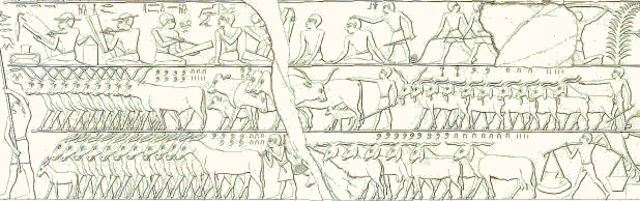
\includegraphics[width=\linewidth]{figuras/ancient_counting.png}
\end{figure} 
\vspace{2mm}

Quando pensávamos que contar não pudesse ficar mais difícil, os computadores surgem, abrindo novas discussões sobre a 
contagem. Entre elas, estavam como armazenar números em uma máquina, como fazer contas nesses aparelhos e até quanto 
poderíamos contar com a ajuda deles. E poucas décadas após essa invenção, a Internet é criada. 

Passamos, portanto, a ficar interessados em monitorar essa rede de computadores e para isso, tínhamos que descobrir 
quantas máquinas diferentes estavam acessando essa rede ou quem eram os aparelhos responsáveis pelo maior fluxo de dados. 
O principal desafio que surgiu nesse contexto, foi o alto volume de dados que precisavam ser processados em tempo real. 
E armazenar todos os dados localmente para em seguida, analisá-los deixou de ser viável devido à lentidão desse processo 
e ao elevado consumo de memória.

Estruturas de dados e algoritmos probabilísticos são uma forma de tentar contornar essa grande quantidade de informação. 
A ideia central é sacrificar a exatidão da resposta com o objetivo de consumir menos memória e tempo de processamento. 
Problemas que podem se beneficiar com soluções probabilísticas são, por exemplo, monitorar quantos usuários diferentes 
acessaram um site em um dado dia, contar quantas palavras distintas foram pesquisadas na última hora em uma plataforma 
de varejo ou armazenar quantas visualizações distintas um artigo teve. 

Uma característica comum desses problemas é que muitas vezes, suas respostas são métricas a serem utilizadas por outros 
sistemas com o intuito de se identificar falhas ou pontos de melhoria. No caso do monitoramento de quantas pessoas 
visitaram uma página web, uma forte queda nas visualizações pode ser um indício que um serviço esteja fora do ar. Nesse 
sentido, essas métricas não precisam ter necessariamente uma precisão de $100\%$, podendo apresentar um pequeno erro 
desde que sejam rapidademente computadas e leves de se armazenarem.

Por volta da década de~1970, Robert Morris tentou contar eventos cujo número de ocorrências não cabia na memória dos 
computadores da época~\citep{morris:78}. O \hyperref[chap:morris:algorithm]{algoritmo} proposto por ele serviu de 
inspiração para que outros autores conseguissem resolver problemas mais desafiadores, como a contagem distinta 
aproximada, cujo objetivo é estimar a quantidade de elementos distintos em um fluxo de dados. 

Alguns anos após Morris publicar o trabalho dele, a \hyperref[sec:flajolet-martin:algorithm]{$\pcounting$}, o primeiro 
algoritmo probabilístico que resolvia a contagem distinta aproximada, foi criada~\citep{flajolet:martin:85}. E a partir 
desse algoritmo, as soluções foram passando por melhorias, das quais podemos destacar a redução do consumo de memória, 
aumento da precisão e até mesmo o desenvolvimento de técnicas de demonstração que simplificavam o entendimento da razão 
desses algoritmos funcionarem.

Pouco tempo depois, as \hyperref[lab:chapter:04:01]{\asampling}, algoritmo que corrigia limitações da solução anterior, 
foram desenvolvidas~\citep{adptive:sampling:90}. Após uma década, a estrutura de dados 
\hyperref[sec:loglog:algorithm]{$\LOG$} é concebida, apresentando uma grande redução no consumo de 
memória~\citep{loglog:03}. E logo em seguida, o \hyperref[sec:loglog:hyperloglog]{$\HLOG$}, versão aperfeiçoada do 
$\LOG$, veio a público e se tornou uma das estruturas mais utilizadas para se resolver o problema da contagem distinta 
aproximada~\citep{hyperloglog:07}. Este texto, portanto, tem o objetivo de passar por essas soluções e apresentar 
comentários pertinentes de cada uma.

\vspace{2mm}
\begin{figure}
  \centering
  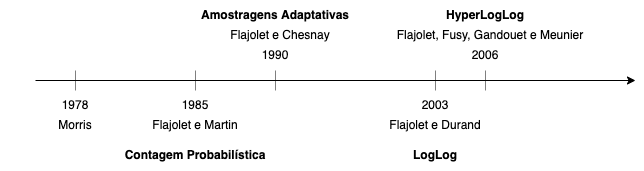
\includegraphics[width=\linewidth]{figuras/count_distinct_timeline.png}
\end{figure}  

\newpage
\section{Probabilidade}

Neste texto, serão discutidas soluções probabilísticas de problemas relacionados à contagem. Para entendê-las, alguns
conceitos relacionados à Estatística precisam estar claros.

\section{Variância}
\label{ap:variance}

Seja $X$ uma variável aleatória. Então,

\[ \mathbb{V}[X] = \mathbb{E}[X^2] - \mathbb{E}[X]^2\]

\section{Desigualdade de Markov}
\label{ap:markov}

Sejam $X$ uma variável aleatória e $\alpha > 0$ um número real. Então,

\[ \mathbb{P}(X \geq \alpha) \leq \frac{\mathbb{E}[X]}{\alpha^2}\]


\section{Desigualdade de Chebyshev}
\label{ap:chebyshev}

Seja $X$ uma variável aleatória com valor esperado $\mu$ finito e variância $\sigma^2$ finita e diferente de zero. 
Assim, para todo número real $k > 0$, 

\[ \mathbb{P}(| X - \mu| \geq k\sigma) \leq \frac{1}{k^2}\]

Outro modo de se escrever a desigualdade acima é 

\[ \mathbb{P}(| X - \mu| \geq k) \leq \frac{\sigma^2}{k^2} \]

\section{Transformação de Mellin}
\label{ap:mellin}

A transformação de Mellin para uma função \textit{real} $f(x)$ definida para $x \in \mathbb{R}$ e $x \geq 0$ é uma função 
\textit{complexa} $f^{*}(x)$ tal que:

\[ f^{*}(s) := M\big[f(x); s\big] = \int_{0}^{\infty} f(x)^{s-1} dx \ .\]
\par

\chapter{Contagem aproximada}
\label{chap:morris}


\section{O Problema}

O problema de contagem aproximada consiste em contar um grande número de eventos usando pouca memória.  
Esse problema foi abordado pela primeira vez por Robert  Morris (Morris, 1978). 
Neste artigo, o autor descreve a tentativa de se contar eventos cujas frequências podiam chegar até 130.000, mas só usando contadores de 8 bits.

Um registrador de n bits pode guardar valores até $2^n-1$. Dessa forma, em uma máquina que possui registradores de 8 bits, pode-se contar até 255.
Assim, o autor não conseguia manter as frequências exatas dos eventos devido à limitação de máquina. 
Contudo, ele podia armazenar contagens aproximadas.


\section{Ideias para solução}

Para se manter um contador exato até $n$, precisa-se de $O(\log n)$ bits. Para se conseguir contar até $n$ usando menos bits, 
deve-se abrir mão da exatidão da contagem. 

Uma das primeiras ideias é manter no contador o valor de $\log_2 n$ e assim, utilizar $O(\log \log n)$ bits de memória. 
A estimativa da contagem seria $2^x$, em que, $x$ é o valor armazenado no contador.

Outra ideia é como deve ser feita o incremento desse contador. 
A solução proposta por Morris é aumentar o contador com base em um método probabilístico, como pode ser visto no Programa \ref{prog:morris}. 


\section{Pseudocódigo}

\begin{programruledcaption}{Contagem aproximada: algoritmo de Morris\label{prog:morris}}
  \begin{lstlisting}[
    language={[brazilian]pseudocode},
    style=pseudocode,
    style=wider,
    functions={},
    specialidentifiers={},
  ]
      funcao Morris(M)  // Estima o tamanho de um conjunto de dados M
        X := 0  // Inicia o contador que guarda o logarítmo na base 2 do tamanho do conjunto M
        para cada dado do conjunto M faça
          para i de 0 até X faça
            jogue uma moeda 
          fim

          se todas as jogadas forem cara faça
            X := X + 1
          fim
        fim
      devolva $2^X - 1$
      fim
  \end{lstlisting}
\end{programruledcaption}

\section{Erro cometido}

Escrever a prova do algorimo \dots

\par

\newcommand{\bitmap}{\text{BITMAP}}
\newcommand{\pcounting}{\textit{probabilistic counting}}

\chapter{Contagem distinta aproximada: Flajolet-Martin (1985)}
\label{lab:flajolet-martin}

\section{O Problema}

\begin{quote}
  \textbf{Contagem Distinta:} Dado um conjunto $\Mbb$, \textbf{encontrar} quantos elementos \textit{distintos}
  $\Mbb$ possui.
\end{quote}

Uma solução para a \textbf{contagem distinta} é inserir cada elemento de $\Mbb$ em uma tabela hash. 
E assim, a quantidade de itens distintos nesse conjunto será o número de elementos nessa tabela.

Note que esse algoritmo consome $\Omega(n)$ de memória, uma vez que, deve-se armazenar cada elemento 
\textbf{pelo menos uma vez} para que seja possível verificar se um item está no conjunto.

Este consumo linear de espaço pode ser um problema quando a quantidade de elementos que precisam ser armazenados é muito 
grande. E podem existir aplicações nas quais é necessário manter \textbf{várias} dessas estruturas, como no caso do 
\textit{Redis}, em que se deseja encontrar quantos usuários distintos visualizararm um publicação ~\citep{Redis}. E para 
essas situações, é interessante que o consumo de memória seja muito menor que a quantidade de elementos distintos. 
Portanto, deve-se abandonar a exatidão da contagem dos elementos distintos para que se possa diminuir o consumo de 
espaço.

\begin{quote}
  \textbf{Contagem Distinta Aproximada:} dado um conjunto $\Mbb$, \textbf{estimar} o número de elementos 
  \textit{distintos} nesse conjunto.
\end{quote}

Uma das primeiras soluções para a \textbf{contagem distinta aproximada} foi apresentada por \textit{Philippe Flajolet} e 
\textit{Nigel Martin} no artigo ~\citep{flajolet:martin:85}.
A motivação para o desenvolvimento desse algoritmo foi a otimização de pesquisas em bancos de dados relacionais.
E a identificação do número de elementos distintos em uma coluna era a principal dificuldade nesse processo.

\section{Algoritmo de Flajolet-Martin}
\label{sec:flajolet-martin:algorithm}

O \textbf{algoritmo de Flajolet-Martin} utiliza uma função de hash $h$ que mapeia uniformemente cada elemento do 
conjunto $\Mbb$ para um número inteiro entre $0$ e $2^L-1$, em que $L$ é a quantidade necessária de bits para 
mapear todas as entradas de $\Mbb$ (na prática, este valor é $32$ ou $64$). Assim, para cada $x_i \in \Mbb$, 
será calculado um inteiro $y_i \coloneqq h(x_i)$. Note que $y_i$ pode ser visto como uma palavra binária aleatória de 
$L$ bits em que cada bit é gerado independentemente com probabilidade $\frac{1}{2}$. E o algoritmo é baseado na 
frequência das aparições dos prefixos dessas palavras aleatórias.

Então, suponha que palavras binárias aleatórias de $L$ bits estejam sendo geradas. Espera-se que a cada \textbf{2} 
palavras, pelo menos uma comece com \textbf{1}. E que a cada \textbf{4} palavras, pelo menos uma deva ter o prefixo 
\textbf{01}. Assim, a cada $\mathbf{2^k}$ palavras, espera-se que pelo menos uma palavra comece com $\mathbf{0^{k-1}1}$. 
Por outro lado, caso o prefixo $0^{k-1}1$ apareça, o esperado é que $2^{k}$ items já devam ter sido gerados. 

Dessa forma, o algoritmo mantém a ocorrência dos prefixos de cada $\textit{hash}$ em um vetor $\bitmap[0 \twodots L-1]$, 
de modo que $\bitmap[i] = 1$, se e somente se, o prefixo $0^i1$ apareceu entre os \textit{hashes} dos elementos de 
$\Mbb$. 

Note que é necessário mapear cada prefixo para um inteiro entre $0$ e $L - 1$. E para isso, defini-se a função $\rho$ 
que recebe um inteiro e devolve a posição do 1 menos significativo deste inteiro. Então, para um \textit{hash} $y$, 
suponha que $\rho(y) = k$. Assim, o prefixo da representação binária de $y$ é $0^k1$, e $\bitmap[k] = 1$. Um caso 
especial para essa função é quando o \textit{hash} é zero. Nesta situação, $\rho(0) = L$.

Por fim, seja $R$ o menor índice tal que $\bitmap[R] = 0$. A estimativa para o número de elementos distintos de 
$\Mbb$ será $2^R/\phi$, em que, $\phi$ é um fator de correção que será discutido em 
\refeq{sec:flajolet-martin:analysis}.

Segue o pseudocódigo:
\begin{programruledcaption}{
Algoritmo de Flajolet-Martin 
\\ \textbf{Entrada:} conjunto $\Mbb$, função de hash $h$, tamanho $L$ do vetor $\bitmap$ 
\\ \textbf{Saída:} quantidade de elementos distintos de $\Mbb$
\label{prog:flajolet-martin}
}
  \begin{lstlisting}[
    language={[brazilian]pseudocode},
    style=pseudocode,
    style=wider,
    functions={},
    specialidentifiers={},
  ]
      funcao FlajoletMartin($\Mbb$, h, L)
        para i de 0 até L \kw{faça}:
          $\bitmap[i]$ := 0
        fim
        para x $\in$ $\Mbb$ \kw{faça}:
          y := h(x)
          $\bitmap[\rho(y)]$ := 1
        fim
        R := 0
        enquanto $\bitmap[R]$ = 1 \kw{faça}:
          R := R + 1
        fim
        devolva $2^R/\phi$
      fim
  \end{lstlisting}
\end{programruledcaption}

\section{Análise do algoritmo}
\label{sec:flajolet-martin:analysis}

Suponha que a quantidade de elementos distintos de $\Mbb$ seja $n$. O valor esperado de $R$ definido na seção 
\refeq{sec:flajolet-martin:algorithm} é aproximadamente $\log_2(\phi n)$, em que $\phi = 0.77351\dots$ e o desvio padrão 
de $R$ é em torno de $1.12$. Essa seção busca mostrar as etapas da análise do Algoritmo~\ref{prog:flajolet-martin} feita 
por Flajolet e Martin. Os detalhes da prova podem ser vistos em ~\citep{flajolet:martin:85}.

O primeiro passo é entender que $R$ é uma estimativa para $\lfloor \log_2(n) \rfloor$. Pelo padrão das aparições dos 
prefixos dos hashes dos elementos de $\Mbb$, espera-se que $\bitmap[0]$ seja acessado aproximadamente $\lfloor 
\frac{n}{2} \rfloor$ vezes, $\bitmap[1]$ aproximadamente $\lfloor \frac{n}{4} \rfloor$ vezes $\dots$ Agora, para 
$k = \lfloor \log_2(n) \rfloor$, $\bitmap[k]$ deve ser acessado em torno de $\lfloor \frac{n}{2^{k+1}} \rfloor = 0$ 
vezes. Assim, o menor índice $R$ tal que o valor de $\bitmap$ seja zero é aproximadamente $\lfloor \log_2(n) \rfloor$.

Então, defini-se a variável aleatória $R_n$ como sendo o valor da variável $R$ ao final da execução do Algoritmo 
\ref{prog:flajolet-martin} para uma entrada $\Mbb$ com $n$ elementos distintos. Dessa forma, o interesse principal 
da demonstração é encontrar fórmulas ou estimativas para:
\begin{itemize}
  \item $p_{n,k} = \mathbb{P}(R_n = k)$: probabilidade de uma saída de \ref{prog:flajolet-martin} ser igual a $k$
  \item $q_{n,k} = \mathbb{P}(R_n \geq k)$: probabilidade de uma saída de \ref{prog:flajolet-martin} 
  ser maior ou igual a $k$
  \item $\Ebb[R_n]$: valor esperado de $R_n$
  \item $\Vbb[R_n]$: variância de $R_n$
\end{itemize}

O primeiro teorema de ~\citep{flajolet:martin:85} mostra uma fórmula \textit{exata} e \textit{discreta} para $q_{n,k}$. 
A principal idea para encontrar essa fórmula é agrupar as palavras binárias por prefixos da forma $0^k1$. Assim, 
defini-se $E_k = \{ x  \ | \ \rho(x) = k \}$, ou seja, $E_k$ é o conjunto de todas as palavras aleatórias com prefixos
iguais a $0^k1$. Da mesma forma, defini-se $K_k = \{ x \ | \ \rho(x) \geq k \}$. Em seguida, as diferentes entradas 
$\Mbb$ com $n$ elementos distintos são representadas por um polinômio:
\[ P_k^{(n)} = (E_0 + E_1 + \twodots + E_{k-1} + K_k)^n .\]

O próximo passo é tentar expandir esse polinômio usando \textit{inclusão e exclusão}, e associar uma medida 
probabilidade para $E_0, E_1, \twodots, E_{k-1}, K_k$. E a prova deste teorema termina encontrando uma relação entre 
$q_{n,k}$ e esta expansão de polinômio.

Em seguida, o Teorema 2 apresenta aproximações de $q_{n,k}$ para diferentes intervalos de $k$. E a consequência deste 
teorema é a existência de uma distribuição limitante para a distribuição de probabilidade de $R_n$ conforme $n$ cresce. 
Dessa forma, obtém-se uma fórmula \textit{aproximada} e \textit{contínua} para $q_{n,k}$:
\[ q_{n,k} \approx \psi(\frac{n}{2^k}) \]

em que, $\psi(x) = \prod_{j \geq 0} (1 - e^{-x2^j})$.

Note que por definição, $p_{n,k} = q_{n,k} - q_{n,k+1}$. Assim, pode-se aproximar $p_{n,k}$:
\[ p_{n,k} \approx \psi(\frac{n}{2^k}) - \psi(\frac{n}{2^{k+1}}) \ . \]

O interesse passa a ser, portanto, estimar $\Ebb[R_n]$ a partir dessa fórmula aproximada de $p_{n,k}$, de maneira 
que 
\[ \Ebb[R_n] = \sum_{k \geq 1} k p_{n,k} \approx \sum_{k \geq 1} k \Big[ \psi \Big( \frac{n}{2^k} \Big) - \psi 
  \Big( \frac{n}{2^{k+1}} \Big) \Big] \ . \]

Desse modo, defini-se a função real $F(x)$ como sendo
\[ F(x) =  \sum_{k \geq 1} k \Big[ \psi \Big( \frac{n}{2^k} \Big) - \psi \Big( \frac{n}{2^{k+1}} \Big) \Big] \ . \]

E o Lema 1 do artigo, afirma que 
\[ \Ebb[R_n] = F(x) + O \Big( \frac{1}{n^{0.49}} \Big) \ , \]
ou seja, que o valor esperado de $R_n$ se aproxima de $F(x)$ conforme $n$ cresce.

Em seguida, o Lema 2 apresenta o resultado da \hyperref[ap:mellin]{transformada de Mellin} de $F(X)$. A principal razão 
para se calcular essa transformação é que se pode expressar a fórmula inversa da transformada de Mellin como uma 
expansão assintótica cujos termos são resíduos da transformada. Assim, o Teorema $3A$ utiliza os Lemas 1 e 2, e o 
Teorema dos Resíduos para afirmar que 
\[ \Ebb[R_n] = \lg (\phi n) + P(\lg n) + o(1) \ , \]
em que, $P(x)$ é a expansão assintótica de $F(x)$ e $\phi = 0.77351\dots$, concluindo a prova que 
$\Ebb[R_n] \approx \lg (\phi n)$.

A prova para a estimativa de $\Vbb[R_n]$ segue os mesmos passos da prova anterior. Pela definição de 
\hyperref[ap:variance]{variância}, precisa-se estimar $\Ebb[R_n ^ 2]$. Assim, 
\[ \mathbb{E[R_n ^2]} = \sum_{k=1} k^2 p_{n,k} \approx G(x) \ , \]
em que
\[ G(x) = \sum_{k=1} k^2 p_{n,k} \ . \]

Dessa forma, encontra-se a transformada de Mellin de $G(x)$ e se analisa a inversa desta transformação para estimar 
$\Ebb[R_n^2]$.

\section{Melhorando precisão do algoritmo}

Na seção anterior, foi visto que $\Ebb[R_n] \approx \lg(\phi n)$, em que $\phi \approx 0.77351$. Assim, se o valor 
do contador $R$ no final do Algoritmo \ref{prog:flajolet-martin} para uma entrada com $n$ elementos distintos for 
aproximadamente igual a $\lg(\phi n)$, então a saída desse algoritmo é aproximadamente $n$. A tabela \ref{tab:flajolet} 
mostra que, em alguns casos, a saída do programa é praticamente igual a $n$ quando $R_n \approx \lg(\phi n)$.

\begin{center}
  \def\arraystretch{2}%
  \begin{table}
    \begin{tabular}{ |p{1.5cm}||p{2.5cm}|  }
      \hline
      \multicolumn{1}{|p{1.5cm}|}{\centering $n$ } 
      & \multicolumn{1}{|p{2.5cm}|}{\centering $(1 \slash \phi) 2^{\lg(\phi n)}$ }  \\
      \hline
      \multicolumn{1}{|p{1.5cm}|}{\centering 50 } 
      & \multicolumn{1}{|p{2.5cm}|}{\centering 49.99 }  \\
      \hline
      \multicolumn{1}{|p{1.5cm}|}{\centering 500 } 
      & \multicolumn{1}{|p{2.5cm}|}{\centering 500.0 }  \\
      \hline
      \multicolumn{1}{|p{1.5cm}|}{\centering 5000 } 
      & \multicolumn{1}{|p{2.5cm}|}{\centering 4999.99 }  \\
      \hline
      \multicolumn{1}{|p{1.5cm}|}{\centering 50000 } 
      & \multicolumn{1}{|p{2.5cm}|}{\centering 50000.0 }  \\
      \hline
     \end{tabular}
     \caption{\label{tab:flajolet} Comparação entre $n$ e saída do Algoritmo \ref{prog:flajolet-martin} para 
     $R_n = \lg(\phi n)$.}
  \end{table}
\end{center}

Contudo, $\Vbb[R_n] \approx\nolinebreak 1.12$ e consequentemente, o desvio padrão de $R_n$ é aproximadamente~$1$. 
Isto quer dizer que o valor de $R_n$ pode ser uma unidade maior ou menor que $\lg(\phi n)$, o que implica que a 
estimativa de $n$ possa ser duas vezes maior ou menor que $n$. Logo, o Algoritmo de Flajolet e Martin apresenta uma 
grande variabilidade.

Assim como foi visto na Seção \ref{sec:morris:plus}, pode-se diminuir a variância da estimativa fazendo $k$ iterações 
do Algoritmo \ref{prog:flajolet-martin}. Dessa forma, seria necessário manter $k$ vetores \bitmap, $k$ valores de $R$ e 
$k$ funções de hash $h$. Ao final de todas as $k$ iterações, seria calculado a média $\bar{R}$ dos valores de $R$, e a 
estimativa do número de elementos distintos seria $(1 \slash \phi) 2^{\bar{R}}$.

O pseudocódigo a seguir codifica essa idea:

\begin{programruledcaption}{
  Algoritmo de Flajolet-Martin+
  \\ \textbf{Entrada:} conjunto $\Mbb$, $k$ funções de hash, tamanho $L$ do vetor $\bitmap$ 
  \\ \textbf{Saída:} quantidade de elementos distintos de $\Mbb$
  \label{prog:flajolet-martin+}
  }
    \begin{lstlisting}[
      language={[brazilian]pseudocode},
      style=pseudocode,
      style=wider,
      functions={},
      specialidentifiers={},
    ]
        funcao FlajoletMartin($\Mbb$, k, h, L)
          para i de 0 até k \kw{faça}:
            para j de 0 até L \kw{faça}:
              $\bitmap_i[j]$ := 0
            fim
          fim
          para i de 0 até k \kw{faça}:
            para x $\in$ $\Mbb$ \kw{faça}:
              y := $h_i(x)$
              $\bitmap_i[\rho(y)]$ := 1
            fim
          fim
          para i de 0 até k \kw{faça}:
            $R_i$ := 0
          fim
          para i de 0 até k \kw{faça}:
            enquanto $\bitmap_i[R_i]$ = 1 \kw{faça}:
              $R_i$ := $R_i$ + 1
            fim
          fim
          $\bar{R}$ := 0
          para i de 0 até k \kw{faça}:
            $\bar{R}$ := $\bar{R} + R_i$ 
          fim
          $\bar{R}$ := $\bar{R} \slash k$
          devolva $2^{\bar{R}}/\phi$
        fim
    \end{lstlisting}
  \end{programruledcaption}

Seja $\bar{R_n}$ o valor da variável $\bar{R}$ ao final da execução do Algoritmo \ref{prog:flajolet-martin+} para uma
entrada com $n$ elementos distintos. De forma análoga aos resultados vistos na Seção \ref{sec:morris:plus}, pode-se
concluir que:
\[ \Ebb[\bar{R_n}] \approx \lg(\phi n)  \; \; \text{e}  \; \; \Vbb[\bar{R_n}] \approx \frac{1.12}{k} \ . \]


No entanto, o fato de se precisar de uma função de hash distinta para cada iteração torna a solução acima inviável, 
uma vez que, encontrar funções de hash que mapeiem na prática os elementos de um conjunto $\Mbb$ de maneira
uniforme não é uma tarefa simples. Para contornar esse problema, os autores propuseram o uso da 
\textit{média estocástica}.

Essa ideia consiste em dividr os elementos da entrada em $k$ lotes e usar parte da informação do hash para definir em 
qual lote um elemento deve ir. 
As linhas de $7$ até $11$ do pseudocódigo a seguir mostram como esta divisão é feita:
\begin{programruledcaption}{
  Algoritmo de Flajolet-Martin++
  \\ \textbf{Entrada:} conjunto $\Mbb$, funções de hash $h$, tamanho $L$ do vetor $\bitmap$, 
  quantidade $k$ de lotes
  \\ \textbf{Saída:} quantidade de elementos distintos de $\Mbb$
  \label{prog:flajolet-martin++}
  }
    \begin{lstlisting}[
      language={[brazilian]pseudocode},
      style=pseudocode,
      style=wider,
      functions={},
      specialidentifiers={},
    ]
        funcao FlajoletMartin($\Mbb$, k, h, L)
          para i de 0 até k \kw{faça}:
            para j de 0 até L \kw{faça}:
              $\bitmap_i[j]$ := 0
            fim
          fim
          para x $\in$ $\Mbb$ \kw{faça}:
            lote := $h(x) \mod k$
            y := $\lfloor h(x) / k \rfloor$
            $\bitmap^{<lote>}[\rho(y)]$ := 1
          fim
          para i de 0 até k \kw{faça}:
            $R_i$ := 0
          fim
          para i de 0 até k \kw{faça}:
            enquanto $\bitmap_i[R_i]$ = 1 \kw{faça}:
              $R_i$ := $R_i$ + 1
            fim
          fim
          $\bar{R}$ := 0
          para i de 0 até k \kw{faça}:
            $\bar{R}$ := $\bar{R} + R_i$ 
          fim
          $\bar{R}$ := $\bar{R} \slash k$
          devolva $k2^{\bar{R}}/\phi$
        fim
    \end{lstlisting}
  \end{programruledcaption}

Se a função de hash $h$ distribuir os $n$ elementos distintos do conjunto $\Mbb$ uniformemente entre os 
$k$ lotes, então espera-se que cada lote tenha aproximadament $\frac{n}{k}$ elementos. Dessa forma, 
$(1 / \phi)2^{\bar{R_n}}$ seria uma aproximação para $\frac{n}{k}$. É devido a este fato que a saída do Algoritmo~
\ref{prog:flajolet-martin++} é $\mathbf{k} (1 / \phi)2^{\bar{R_n}}$, pois este valor é uma estimativa para 
$\mathbf{k} \frac{n}{k} = n$.

Por fim, o erro relativo esperado do algoritmo \proc{ProbabilisticCounting++} é em torno de $0.78 / \sqrt{m}$. Isto quer 
dizer que para $m = 64$, o desvio esperado é em torno de $10\%$. Dessa forma, a escolha de $m$ depende das exigências do 
problema. Se precisarmos de uma precisão maior, escolheremos um valor de $m$  maior, mas teremos um algoritmo mais 
custoso em termos de tempo e espaço. Por outro lado, se a exigência é, por exemplo, decidir qual de dois conjuntos tem a 
menor quantidade de elementos distintos, podemos escolher um valor menor de $m$ para fazer essa comparação, mas teríamos 
um risco maior de escolher o conjunto errado.

\section{Limitações do algoritmo $\pcounting$}

Uma das principais razões para escolhermos algoritmos \textit{probabilísticos} ao invés de algoritmos \textit{exatos} é 
o \textbf{consumo de memória reduzido}. Por exemplo, para resolver o problema da contagem distinta de forma 
\textit{exata}, podemos manter uma tabela de hash e conforme os elementos forem processados, adicionar a esta tabela 
somente aqueles elementos que não apareceram ainda. Assim,  quantidade de elementos distintos processados será o tamanho 
da tabela. Suponha que cada hash seja um inteiro de 4 bytes (32 bits) e que existam um milhão de itens distintos 
percorridos. Para armazenar essa tabela, gastaríamos pelos menos 4 MB. Por outro lado, se usarmos o algoritmo 
$\pcounting$ para resolver esse problema, o consumo de memória seria proporcional ao valor $m$ e não dependeria da 
quantidade de itens distintos. Logo, se o vetor $\bitmap$ for um vetor de inteiros de 4 bytes de tamanho $m$, e 
$m$ for igual a 1024, então a memória consumida por esse algoritmo seria em torno de 4 KB, que é um consumo de espaço
\textbf{1000 vezes menor} que a solução exata.

O erro relativo esperado do $\pcounting$ para $m = 1024$ é em torno de $2{,}5\%$. Assim, para um conjunto de milhões de 
itens distintos, o erro seria em torno das dezenas ou centenas de milhares. Com esse tipo de desvio, teríamos como 
mensurar a ordem de grandeza do número de itens distintos de um conjunto com bastante confiança. Contudo, para utilizar
o $\pcounting$, o viés desse algoritmo deve ser entendido.

O \textbf{viés} de um estimador é a diferença entre seu valor esperado e o valor real do parâmetro estimado. Nesse sentido, a 
estimativa da quantidade de elementos em um conjunto devolvida pelo algoritmo de \proc{Morris} é \textit{não-viesada}, 
uma vez que, o Lema \ref{morris:expected_value} afirma que o valor esperado deste estimador é igual ao tamanho do 
conjunto estimado.

Na prova descrita em ~\citep{flajolet:martin:85}, o estimador de $\lg(n)$ é $R_n$, que representa o valor da variável 
$R$ ao final da execução de \proc{ProbabilisticCounting}, tendo como entrada um conjunto com $n$ elementos distintos. 
Vimos que o valor esperado de $R_n$ é aproximadamente $\lg(\phi n)$, que é diferente de $\lg(n)$. Portanto, $R_n$ é um 
estimador \textit{viesado} de $\lg(n)$. E analogamente, o estimador devolvido por \proc{ProbabilisticCounting++} também 
é \textit{viesado}.  

Então, além do erro padrão, existe também o viés do algoritmo $\pcounting$, cujo valor é $1 + 0{,}31/m$. Contudo, para 
valores de $m$ maiores que $32$, o viés se torna desprezíval se comparado ao erro padrão. Dessa forma, uma pessoa pode 
ser induzida a concluir que a escolha de $m$ é o único cuidado que ela deve tomar ao utilizar esse algoritmo. No 
entanto, ainda existe o problema de estimar \textit{baixas cardinalidades} com essa estrutura.

Suponha, portanto, que $m = 64$ e que o hash do único elemento de um conjunto $\Mbb$ comece com $1$. Logo, se passarmos 
$\Mbb$ para \proc{ProbabilisticCounting++}, existiria um vetor $\bitmap$ cuja primeira posição teria o valor $1$, e o 
restante dos vetores $\bitmap$ teriam todos valores zero. Assim, $\bar{R}$ será igual a $1/64$, e o estimador de $n$ 
terá o valor de $64 \ 2^{\frac{1}{64}}/\phi \approx 83.64$. Esta estimativa está muito distante do valor real, que é 
$n = 1$.

Em vista disso, um tratamento especial deve ser dado para situações em que a cardinalidade do número de elementos 
distintos de um conjunto for baixa. Poderíamos, por exemplo, manter os elementos percorridos em uma tabela de hash, e 
quando essa tabela atingisse um certo tamanho, passaríamos a usar a estratégia original do $\pcounting$, que é preencher
os vetores $\bitmap$.  
\par

\newcommand{\asampling}{\proc{Amostragens Adaptativas}}
\newcommand{\AS}{\proc{AdaptiveSampling}}

\chapter{Contagens por amostragens}

Este capítulo aborda uma outra solução para o problema da contagem distinta aproximada. O 
Capítulo~\ref{lab:flajolet-martin} apresentou o algoritmo da $\pcounting$, que estima o número de elementos distintos em 
um fluxo de dados com desvio padrão em torno de $0.78 / \sqrt{m}$. 

O algoritmo das $\asampling$ tem um desvio padrão de aproximadamente $1.20 / \sqrt{m}$~\citep{adptive:sampling:90}. 
As razões para estudarmos esse algoritmo mesmo que ele apresente um erro maior ficarão claras nas próximas seções.

\section{Algoritmo das $\asampling$}
\label{lab:chapter:04:01}

O algoritmo das $\asampling$ também se baseia em \hyperref[sec:flajolet-martin:pattern]{padrões de bits} dos hashes dos 
elementos examinados. Podemos dessa forma, considerar que os elementos que estamos contando são palavras binárias de 
tamanho infinito. 

Enquanto que no algoritmo da $\pcounting$, estávamos interessados na \textbf{aparição} de um elemento com 
prefixo da forma $0^*1$, no algoritmo das $\asampling$, queremos saber a \textbf{quantidade} de elementos com um certo 
prefixo $0^*$.

Nesse sentido, vamos manter um contador $\delta$ cujo valor inicialmente é zero, e uma lista que armazena elementos com 
prefixo $0^{\delta}$. Para cada elemento examinado, inserimos ele na lista se o prefixo dele for da forma $0^{\delta}$.
Quando essa lista tiver mais que $m$ elementos, incrementamos $\delta$ em 1 e passamos a manter 
somente elementos com prefixo $0^{\delta + 1}$.

Agora, suponha que em um dado momento do algoritmo, a lista tenha tamanho $l$ e estamos mantendo somente elementos com 
prefixos $0^{\delta}$. A probabilidade de um elemento ter um prefixo dessa forma é $1 / 2^{\delta}$, e consequentemente,
esperamos que a cada $2^{\delta}$ itens, pelo menos um item tenha um prefixo desse formato. Assim, se nossa lista tem
$l$ elementos com prefixo $0^{\delta}$, então devemos ter examinado pelo menos $2^{\delta} l$ itens, e este valor é 
justamente a estimativa para a quantidade de valores distintos.

O algoritmo $\AS$ recebe um fluxo $\Mbb$ com $n$ elementos distintos e um parâmetro $m$, que está relacionado com o 
consumo de memória do algoritmo e sua precisão. O algoritmo usa uma função de hash $h$ para associar de forma uniforme 
os elementos de~$\Mbb$ a inteiros de~$L$ bits, e quanto maior for este valor, menor será a quantidade de colisões. Por 
fim, o valor devolvido é um estimador~$\hat{n}$ para $n$ da forma $2^{\delta} l$, em que $l$ e $\delta$ indicam que 
estão sendo armazenados $l$ elementos cujos prefixos tem formato~$0^{\delta}$. 

\begin{codebox}
  \Procname{$\AS(\Mbb, m)$}
  \li $LIST \gets \emptyset$
  \li $\delta \gets 0$
  \li \For cada $x$ em $\Mbb$ 
  \li    \Do 
         \If $0^{\delta}$ é prefixo de $h(x)$ \textbf{e} $h(x) \not\in LIST$
  \li             \Then $LIST \gets LIST \cup \{ h(x) \}$
         \End
  \li    \While $|LIST| > m$                                   \label{li:as:while}
  \li    \Do
         $\delta \gets \delta + 1$
  \li    $TEMPLIST \gets \emptyset$
  \li    \For cada $y$ em $LIST$
  \li    \Do
            \If $0^{\delta}$ é prefixo de $h(y)$
  \li       \Then $TEMPLIST \gets TEMPLIST \cup \{ h(y) \}$
            \End
         \End
  \li    $LIST \gets TEMPLIST$
         \End 
      \End
  \li
  \Return $2^{\delta} |LIST|$   
  \End
\end{codebox}


\section{Vantagens das $\asampling$}
\label{lab:chapter:04:02}

Vamos simular um exemplo pequeno para ver o funcionamento do algortimo $\AS$. Assim, queremos estimar quantos elementos 
distintos o fluxo $\Mbb = \{ 36, 108, 41, 82, 71, 61, 5, 54, 10 \}$ possui. Vamos considerar que a função de hash~$h$ é
a identidade, ou seja, $h(x) = x$ para todo $x$ em $\Mbb$, e que $m = 3$. 

Inicialmente, a lista $LIST$ está vazia e $\delta = 0$. Na primeira iteração do algoritmo, temos que verificar se o 
prefixo da representação binária do elemento $36 = 001001_2$ é da forma $0^0$. Note que qualquer elemento passará nessa 
validação quando $\delta$ for zero, uma vez que, uma palavra binária precisar ter o prefixo $0^0$ significa que ela tem 
que começar com 0 zeros, ou seja, pode começar com 0 ou com 1. Dessa forma, podemos inserir o elemento $36$ na lista, de 
modo que $LIST = \{ 36 \}$. Na próxima iteração, temos que fazer a mesma verificação anterior, só que usando o item de 
valor 108. Novamente, como $\delta = 0$, podemos adicionar $108$ à lista. Analogamente, podemos incluir os elementos 
$41$ e $82$ em $LIST$. 

Contudo, na quarta iteração, entramos no \texttt{while} da linha~\ref{li:as:while}, já que $|LIST| = 4 > m = 3$. Por 
conta disso, incrementamos o valor de $\delta$ e devemos manter em $LIST$ somente aqueles valores cujos prefixos de suas 
representações binárias são da forma $0^{1}$. Vamos ver quais elementos estão em $LIST$:
\[ 
       LIST = \{ 36 = 001001_2, 108 = 0011011_2, 41 = 100101_2, 82 = 0100101_2 \} \  .        
\] 
Precisamos manter nessa lista, somente aqueles números com prefixos que começam com~0. Assim, temos que remover o valor 
41 de $LIST$. 

Continuando o exemplo, precisamos verificar se adicionaremos $71 = 1110001_2$ na lista. Agora, os elementos em $LIST$ 
precisam começar com zero, logo 71 não é inserido. A mesma situação ocorre para os valores $61 = 101111_2$ e 
$5 = 101_2$. Em seguida, podemos inserir $54 = 011011_2$ em $LIST$ e como novamente, $|LIST| = 4 > 3$, teremos que 
incrementar $\delta$ e filtrar os itens da lista. A lista atual é 
\[ \{ 36 = 001001_2, 108 = 0011011_2, 82 = 0100101_2, 54 = 011011_2 \} \ . \] 
Manteremos somentes os valores cujos prefixos binários se iniciam com dois zeros e portanto, 
\[ LIST = \{ 36 = 001001_2, 108 = 011011_2 \} \ . \]
Por fim, o valor $10 = 0101_2$ não é inserido na lista. E a estimativa para a quantidade de elementos distintos em 
$\Mbb$ é $2^{\delta} \times |LIST| = 2^2 \times 2 = 8$. Essa estimativa está cometendo um erro de um item, já que $\Mbb$
tem 9 itens distintos. 

O fato curioso desse exemplo acontece nas primeiras iterações, quando $\delta$ tem valor zero. Vimos que qualquer 
elemento de $\Mbb$ nessas primeiras iterações é inserido em $LIST$. Nessas situações, a estimativa do algoritmo é 
$2^{\delta} \times |LIST| = 2^{0} \times |LIST| = |LIST|$. Ou seja, para os primeiros $m$ itens distintos de $\Mbb$, a 
estimativa tem precisão de $100\%$. Isto é o principal diferencial do algoritmo das $\asampling$ para o algoritmo da 
$\pcounting$, que como foi visto em \hyperref[sec:fm:low_estimates]{Estimando valores pequenos com a $\pcounting$}, 
apresenta um erro muito grande quando queremos estimar cardinalidades baixas.

Outro fator importante de se destacar é que o estimador devolvido por $\AS$ é 
\textbf{não-viesado}~\citep{adptive:sampling:90}. Essa característica está relacionada com o fato do algoritmo das 
$\asampling$ poder estimar valores pequenos sem problemas.

\newpage
\section{Implementando $\asampling$}

Nesta seção apresentaremos a implementação do algoritmo das \proc{Amostragens} \proc{Adaptativas} e experimentos.

\begin{lstlisting}[style=mypython,caption=Implementação do algoritmo $\AS$,captionpos=b, label=as:code]
class AdaptiveSampling:
    def __init__(self, m=64, L=64):
        self.delta: int = 0
        self.m: int = m
        self.L: int = L
        self.LIST: Set[int] = set()
   
    def zeros_no_prefixo(self, x: int):
        return (x & -x).bit_length() - 1

    def adiciona(self, x: int):
        if x not in self.LIST and self.zeros_no_prefixo(x) >= self.delta:
            self.LIST.add(x)

        while len(self.LIST) > self.m:
            self.delta = self.delta + 1
            temp: Set[int] = set()

            for y in self.LIST:
                if self.zeros_no_prefixo(y) >= self.delta:
                    temp.add(y)

            self.LIST = temp

    def conta(self):
        return (1 << self.delta) * len(self.LIST)
\end{lstlisting}

Vamos comentar alguns aspectos do código do Programa~\ref{as:code} baseado no algoritmo~$\AS$. O primeiro detalhe de 
implementação desse programa é que a função de hash~$h$ é implicitamente a função identidade, uma vez que, estamos 
supondo que os elementos inseridos são inteiros gerados uniformemente. O próximo detalhe é a estrutura de dados 
utilizada para representar a lista $LIST$. Foi escolhido um \proc{Set} para representá-la, que é uma estrutura padrão do 
\proc{Python} que permite inserir elementos e verificar se um elemento está presente nela em tempo constante. Dessa 
forma, a complexidade do método~\texttt{adiciona} é $O(1)$ amortizado.

Por fim, falta esclarecer como foi codificada a verificação se um inteiro tem prefixo da forma $0^{\delta}$, ou em 
outras palavras, se a representação binária de um inteiro começa com pelo menos $\delta$ zeros. Lembremos dessa forma, 
da função $\rho$ definida na Seção~\ref{sec:flajolet-martin:algorithm}. Essa função recebe um inteiro $x$ e devolve a 
posição indexada a partir do zero do bit menos significativo de $x$. Assim, $\rho(12) = \rho(0011_2) = 2$ e 
$\rho(24) = \rho(00011_2) = 3$. Note que a saída da função $\rho$ corresponde também a quantidade de bits zeros no 
prefixo da representação binário de um inteiro. Podemos, portanto, aproveitar o método $p$ da classe 
\texttt{ProbabilisticCounting} para implementar o método \texttt{zeros\_no\_prefixo} e agora, para verificar se um 
inteiro~$x$ tem prefixo da forma $0^{\texttt{delta}}$, basta testar se \texttt{zeros\_no\_prefixo(x)} é maior ou igual a
\texttt{delta}.

A partir deste ponto, apresentaremos experimentos do algoritmo das \proc{Amostragens} \proc{Adaptativas}, que serão os 
mesmos realizados na Seção~\ref{sec:fm:experiments}, só que utilizando a estrutura apresentada nesse capítulo. Assim, o 
primeiro experimento que veremos é observar a evolução das estimativas devolvidas pela estrutura
~\texttt{AdaptiveSampling} conforme mais itens são inseridos nela. Portanto, nas simulações realizadas, inserirmos um 
milhão de inteiros de 64 bits distintos gerados uniformemente em estruturas com $m = 64$ e $m = 1024$. E o mesmo gerador 
de números pseudo-aleatórios dos experimentos do algoritmo da~$\pcounting$ foi utilizado, ou seja, os mesmos elementos 
foram aproveitados.

Os resultados do primeiro experimento podem ser observados na Figura~\ref{fig:as:experimento:01}. É possível perceber
que a estrutura com o parâmetro $m$ maior teve uma precisão melhor que a estrutura com $m$ menor ao longo de toda a 
simulação. 

\begin{figure}
  \centering
  \begin{subfigure}{.5\textwidth}
    \centering
    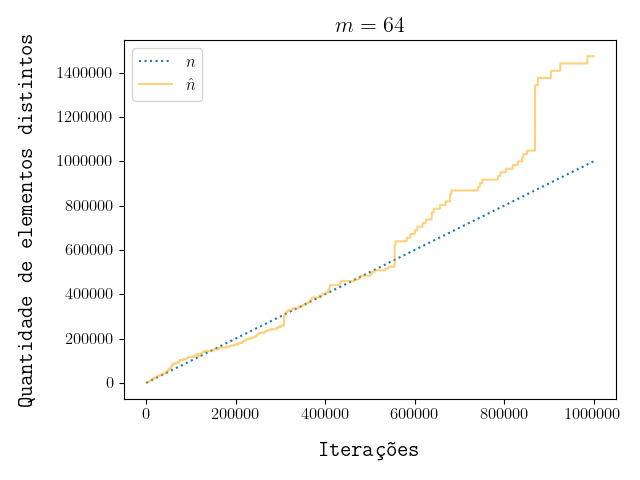
\includegraphics[width=\linewidth, height=4cm]{figuras/adaptive_sampling_full_64.png}
  \end{subfigure}%
  \begin{subfigure}{.5\textwidth}
    \centering
    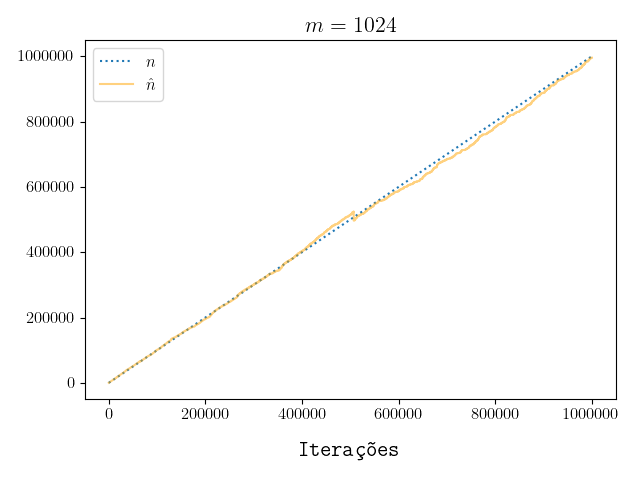
\includegraphics[width=\linewidth, height=4cm]{figuras/adaptive_sampling_full_1024.png}
  \end{subfigure}
  \caption{Primeiro experimento do algoritmo $\AS$. Foram inseridos em estruturas \texttt{AdaptiveSampling} com $m = 64$ 
  e $m = 1024$, um milhão de inteiros de 64 bits gerados uniformemente.}
  \label{fig:as:experimento:01}
\end{figure}


Os gráficos com a evolução do erro relativo do experimento anterior estão na Figura~\ref{fig:as:experimento:01:erro}.
O desvio padrão do algoritmo das $\asampling$ é $1.20/\sqrt{m}$. Portanto, para a estrutura com $m = 64$, o desvio 
padrão é de $15\%$. As estimativas devolvidas por essa estrutura ficaram entre dois desvios padrões na maior parte da 
simulação, apresentando um erro maior quando esta se aproximava do fim. Já a estrutura com $m = 1024$ tem desvio padrão 
de $3{,}75\%$, e a simulação dela teve valores que ficaram dentro de um desvio na maior parte das iterações.

\begin{figure}
  \centering
  \begin{subfigure}{.5\textwidth}
    \centering
    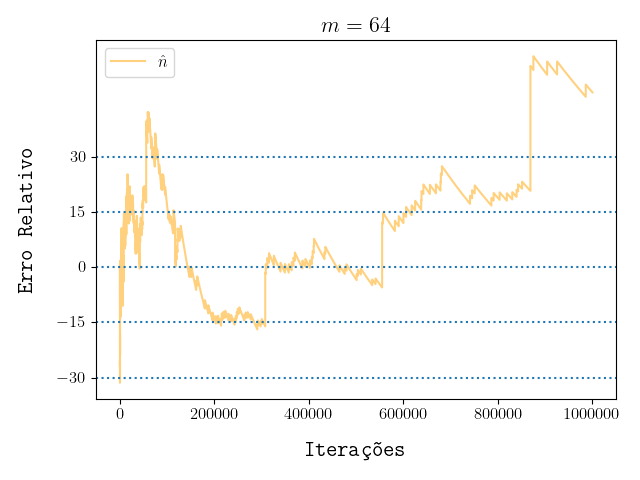
\includegraphics[width=\linewidth, height=4cm]{figuras/adaptive_sampling_erro_full_64.png}
  \end{subfigure}%
  \begin{subfigure}{.5\textwidth}
    \centering
    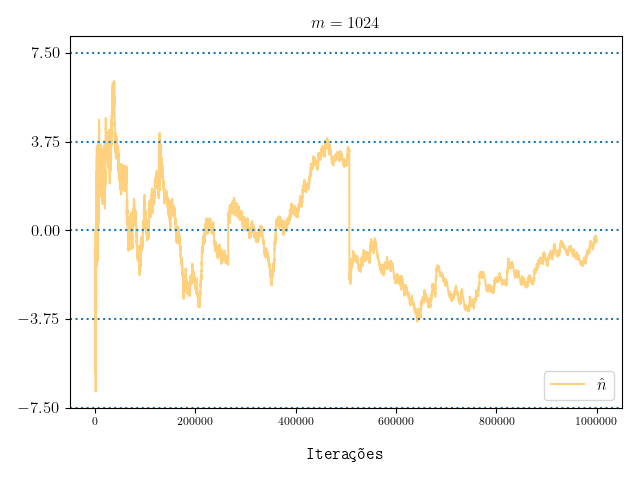
\includegraphics[width=\linewidth, height=4cm]{figuras/adaptive_sampling_erro_full_1024.png}
  \end{subfigure}
  \caption{Erro relativo do primeiro experimento do algoritmo $\AS$. Para $m = 64$, o erro ficou dentro de dois desvios
  padrões. Para $m = 1024$, a faixa de erro foi de um desvio padrão.}
  \label{fig:as:experimento:01:erro}
\end{figure}

Antes de passarmos para o segundo experimento, é interessante verificarmos se o que foi discutido na 
Seção~\ref{lab:chapter:04:02} pode ser observado nas simulações anteriores. Queremos, assim, averiguar se o algoritmo 
das~$\asampling$ funciona de fato para baixas cardinalidades. A Figura~\ref{fig:as:experimento:01:erro:first} tem
gráficos que destacam o erro relativo nas primeiras~256 iterações no caso da estrutura com $m = 64$ e nas primeiras~1024
iterações no caso da estrutura com $m = 1024$. Nos dois casos, podemos notar que o erro relativo nas primeiras~$m$ 
iterações é de fato zero e que o erro após essas iterações iniciais se manteve controlado, dentro da faixa de dois 
desvios padrões.

\begin{figure}
  \centering
  \begin{subfigure}{.5\textwidth}
    \centering
    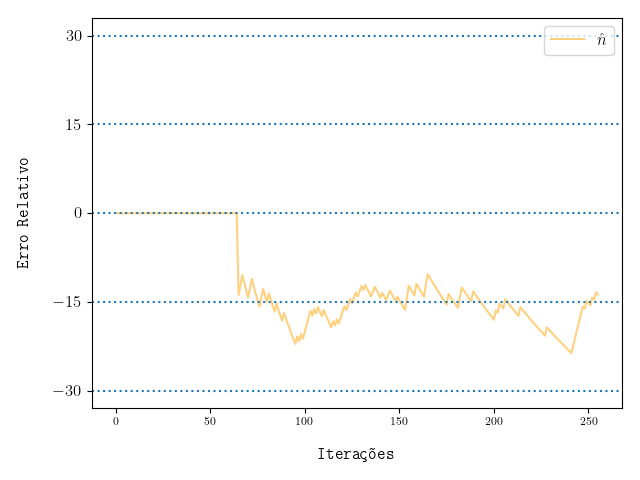
\includegraphics[width=\linewidth, height=4cm]{figuras/adaptive_sampling_erro_first_64.png}
  \end{subfigure}%
  \begin{subfigure}{.5\textwidth}
    \centering
    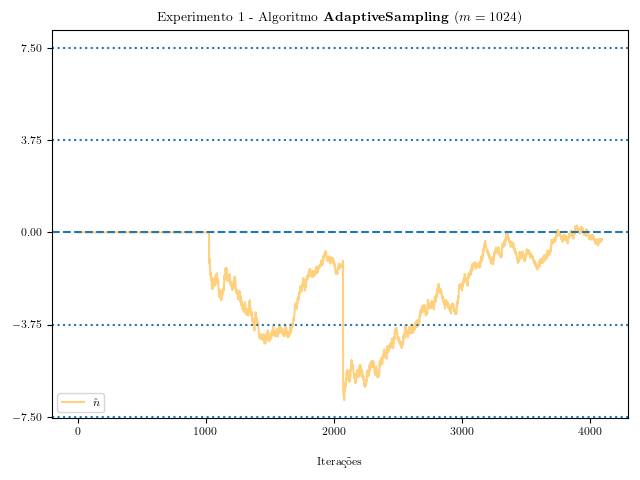
\includegraphics[width=\linewidth, height=4cm]{figuras/adaptive_sampling_erro_first_1024.png}
  \end{subfigure}
  \caption{Erro relativo nas primeiras iterações do experimento do algoritmo~$\AS$. Nas $m$ inserções iniciais,o erro 
  relativo do algoritmo é zero.}
  \label{fig:as:experimento:01:erro:first}
\end{figure}

Para o segundo experimento, repetimos as simulações anteriores dez mil vezes. No final do processo, construímos 
histogramas a partir das frequências das estimativas devolvidas. A Figura~\ref{fig:as:experimento:02} tem as 
distribuições das estimativas da estrutura~\texttt{AdaptiveSampling} com $m = 64$ e $m = 1024$. Nos dois casos, quase 
todos as estimativas ficaram dentro de dois desvios padrões, e houve uma grande concentração de estimativas entre um 
desvio padrão. E podemos notar que com um valor de $m$ maior, a variância do algoritmo das $\asampling$ diminuiu.

\begin{figure}
  \centering
  \begin{subfigure}{.5\textwidth}
    \centering
    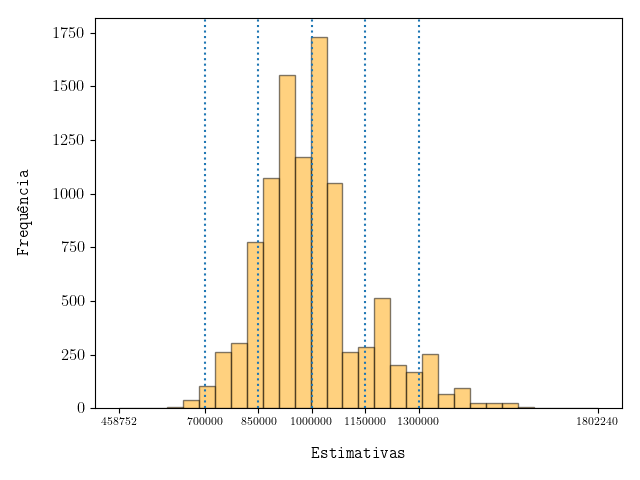
\includegraphics[width=\linewidth, height=4cm]{figuras/adaptive_sampling_variance_64.png}
    \label{fig:as:experimento:02:64}
  \end{subfigure}%
  \begin{subfigure}{.5\textwidth}
    \centering
    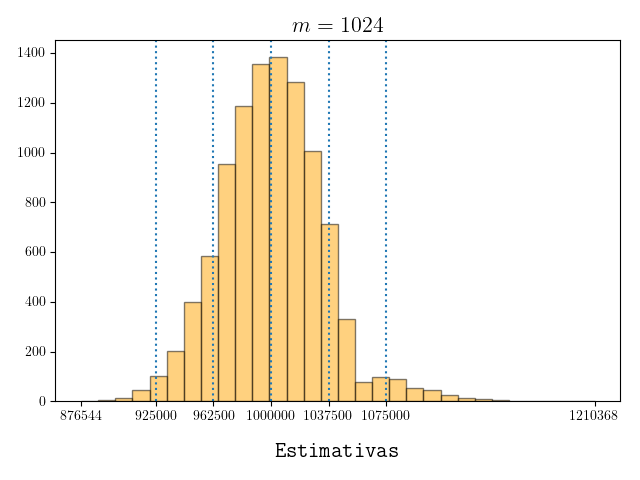
\includegraphics[width=\linewidth, height=4cm]{figuras/adaptive_sampling_variance_1024.png}
    \label{fig:as:experimento:02:1024}
  \end{subfigure}
  \caption{Segundo experimento do algoritmo $\AS$. Foram realizadas dez mil simulações e em cada simulação, foram 
    inseridos em estruturas~\texttt{AdaptiveSampling} com $m = 64$ e $m = 1024$, um milhão de inteiros de~64 bits 
    gerados uniformemente. Os resultados foram utilizados para a construção dos histogramas de frequência acima. }
  \label{fig:as:experimento:02}
\end{figure}

Com os experimentos apresentados nessa seção, foi possível termos noção da precisão do algoritmo das~$\asampling$. Este
algoritmo tem pontos interessantes, como se basear em padrões de bits para construir a estimativa e funcionar bem para
fluxos com poucos elementos. Porém, a principal desvantagem dessa solução é o consumo de memória. Se considerarmos uma
aplicação que precise lidar com hashes de 32~bits, então o consumo de memória da estrutura~\texttt{AdaptiveSampling} 
seria de pelos menos $32 \times m$~bits no pior caso, quando a lista $LIST$ passa a ter mais que $m$ elementos. Esse
custo é o mesmo que o do algoritmo~$\pcounting$, quando $L = 32$. Dessa forma, as $\asampling$, que tem um desvio maior
que a $\pcounting$, tem também um consumo de espaço pior. 

Para que esse gasto de memória fosse reduzido sem que se perdesse muita precisão, demorou mais de 20 anos desde a 
criação da $\pcounting$. Veremos na próxima seção como podemos reduzir ainda mais esse consumo.

\par

\chapter{\textbf{LogLog's}}

Em 1978, Morris resolveu o problema de estimar quantos elementos passaram por um fluxo de dados sem armazenar esse valor 
em um contador. E as ideias principais da \hyperref[chap:morris:algorithm]{solução dele} era guardar uma aproximação do 
logarítmo dessa quantidade e incrementá-la por meio de um método probabilístico que lembra lançamentos de moedas. Dessa 
forma, se temos um fluxo com $n$ elementos, e $X$ é a aproximação do algoritmo de Morris para~$\lg n$, então $X$ deve 
ser incrementado com probabilidade $1 \mathbin{/} 2^X$ para cada novo elemento, e isto é equivalente a lançarmos uma 
moeda $X$ vezes e aumentar $X$ somente se todas as jogadas forem cara. 

Essa solução inspirou o desenvolvimento do algoritmo da $\pcounting$, que resolvia o problema de estimar a quantidade de 
elementos distintos que passaram por um fluxo~$\Mbb$. Nesse \hyperref[sec:flajolet-martin:algorithm]{algoritmo}, estamos 
interessados em usar \hyperref[sec:flajolet-martin:pattern]{padrões de bits} de números inteiros aleatórios para gerar 
essa estimativa. Portanto, os dados de $\Mbb$ são mapeados para inteiros por meio de uma função de hash, e assim, 
podemos considerar que esses elementos são na verdade palavras binárias de tamanho infinito. Essa simplificação nos 
permite agrupar os itens de $\Mbb$ por prefixos da forma $0^{*}1$. A razão de fazermos isto é que a probabilidade de a 
representação binária de um inteiro ter um prefixo da forma $0^{X-1}1$ é $1 \mathbin{/} 2^{X}$, a mesma que aparece no 
algoritmo de Morris, e portanto, essa ideia pode ser usada para estimarmos o logarítmo da quantidade de elementos 
distintos em $\Mbb$ da seguinte forma: guardaremos o menor $R$ tal que ainda não tenha aparecido algum inteiro com 
prefixo~$0^{R}1$.

Dessa maneira, para um fluxo $\Mbb$ com $n$ elementos distintos, $R$ seria a estimativa para~$\lg n$. No entanto, por 
meio do cálculo do valor esperado desse estimador, é possível concluir que $R$, na verdade, não estima $\lg n$, mas 
$\lg \phi n$~\citep{flajolet:martin:85}. Em outras palavras, o algoritmo da $\pcounting$ produz uma estimativa com um 
desvio $\phi$ mensurável e podemos, em vista disso, corrigí-lo.

Contudo, mesmo corrigindo esse erro do estimador, este ainda possui uma grande variância, ou seja, a estimativa 
devolvida pode estar muito próxima ou muito longe do valor real. Para contornar essa situação, podemos repetir várias 
vezes o algoritmo da $\pcounting$ e encontrar a média dos estimadores. E uma forma interessante de se fazer isso em uma 
única iteração, removendo assim, a necessidade de executarmos o algoritmo muitas vezes, é dividir de modo uniforme os 
dados do fluxo em $m$ lotes. Então, um inteiro $x$ faria parte do lote $x \bmod m$, e olharíamos para o prefixo de 
$\lfloor x \mathbin{/} m \rfloor$. Desse modo, passaríamos a guardar um estimador $R$ para cada lote, e a estimativa 
para $n$ usaria a média desses valores. Essa técnica é conhecida como \textbf{média estocástica}.

Por fim, o algoritmo da $\pcounting$ tem consumo proporcional a $O(mL)$ bits, em que $m$ é o número de lotes e $L$ é a
quantidade de bits necessária para armazenar algum inteiro do fluxo. Esse consumo é decorrente do fato de cada lote 
precisar guardar a informação se um prefixo da forma $0^{*}1$ já apareceu, e podemos fazer isto com $L$ bits por lote. 
Nesse sentido, o próximo algoritmo, chamado $\LOG$, terá como base muitas ideias da $\pcounting$, e apresentará uma 
significativa redução do consumo de espaço.

\section{Algoritmo $\LOG$}
\label{sec:loglog:algorithm}

Dado um fluxo $\Mbb$ com $n$ elementos distintos, o algoritmo~$\LOG$ devolverá um estimador~$\hat{n}$ para $n$, que terá
um desvio padrão de $1{,}30 \mathbin{/} \sqrt{m}$~\citep{loglog:03}. Assim como foi feito no algoritmo da $\pcounting$, 
precisamos ter uma função de hash~$h$ que mapeie uniformemente os dados de um fluxo para inteiros. Tendo esta função em 
mãos, podemos supor que estamos trabalhando com um fluxo de inteiros aleatórios. E vamos manter o maior~$M$ tal que 
exista algum elemento em~$\Mbb$ cuja representação binária tenha prefixo da forma $0^{M-1}1$.

Para $M \geq 1$, a probabilidade de um inteiro ter um prefixo da forma~$0^{M-1}1$ é $1 \mathbin{/} 2^{M}$, ou seja, 
esperamos que um em cada $2^{M}$ elementos tenha esse prefixo. Por outro lado, podemos inverter essa ideia, e pensar que 
se temos um inteiro com prefixo da forma $0^{M-1}1$, então pelo menos $2^{M}$ elementos distintos devem ter aparecido. 
Desse modo, o valor de $M$ será uma aproximação para~$\lg n$, e podemos interpretá-lo como sendo a posição indexada a 
partir do 1 do bit ligado menos significativo de um inteiro. Uma ideia similar foi vista na 
Seção~\ref{sec:flajolet-martin:algorithm}, em que definimos a função $\rho$ que retorna a posição indexada a partir 0 do 
bit ligado menos significativo de um número. Em vista disso, vamos definir a função $\rho_1$ que retorna o valor 
anterior só que indexado a partir do 1, e utilizá-la para o cálculo de~$M$.

Para reduzirmos a variância da estimativa, dividimos o fluxo~$\Mbb$ em $m = 2^{k}$ lotes de acordo com os bits dos 
elementos. Dessa forma, um inteiro $x = \langle b_1 b_2 {\dots} b_k {\dots} \rangle$ fará parte do lote 
$y = \langle b_1 b_2 {\dots} b_k \rangle$, ou seja, os $k$ primeiros bits de um elemento indicam em qual lote ele 
pertence. Em seguida, encontramos $M_y$ tal que $0^{M_y}1$ é prefixo de $\langle b_{k+1} b_{k+2} {\dots} \rangle$, e 
mantemos o maior valor de $M_y$.

Desse modo, o valor de $M_y$ de cada lote~$y$ será uma estimativa para $\lg \frac{n}{m}$. Para diminuirmos a variância 
dessa aproximação, calculamos a média \textbf{aritmética} $\overline{M} = \frac{\sum_y M_y}{m}$. Logo, $\overline{M}$ 
aproxima $\lg \frac{n}{m}$, e consequentemente, $2^{\overline{M}}$ aproxima $\frac{n}{m}$. E, portanto, a estimativa 
para $n$ será $m \times 2^{\overline{M}}$.

No entanto, essa estimativa apresenta um desvio e para corrigí-lo, multiplicamos ela por uma constante $\alpha_m$ cujo 
valor é proporcional ao número de lotes utilizados no algoritmo. Na prática, podemos usar como fator de correção 
$\alpha_\infty \approx 0{,}39701$ assim que $m$ for maior que~64. Em vista disso, a saída do algoritmo~$\LOG$ será um 
estimador $\hat{n}$ da forma $\alpha_m \times m \times 2^{\overline{M}}$. E o pseudocódigo a seguir condensa as ideias 
apresentadas.

\begin{codebox}
  \Procname{$\logprogram\big(\Mbb, m = 2^k\big)$}
  \li \For $i$ de $0$ até $m$
        \Do
  \li   $M[i] \gets 0$
        \End
  \li \For cada $x$ em $\Mbb$ 
        \Do
  \li   $b_1b_2{\dots} \gets h(x)$
  \li   $lote \gets \langle b_1 {\dots} b_k \rangle$
  \li   $M[lote] \gets \max(M[lote], \rho_1(b_{k+1}b_{k+2}{\dots}))$
        \End
  \li
  \Return $\alpha_m \times m \times 2^{\frac{1}{m}\sum_i{M[i]}}$   
  \End
\end{codebox}

Vamos simular um exemplo pequeno para entendermos com mais detalhes o algoritmo~$\logprogram$. O objetivo, portanto, é 
estimar a quantidade de elementos distintos em $\Mbb = \{ 50, 85, 45, 29, 89, 82, 87, 10, 92 \}$. Suponhamos que 
$k = 2$, $m = 2^{k} = 2^2 = 4$, que a função de hash~$h$ seja a função identidade e que $\alpha_m = \alpha_4 = 1$, 
ou seja, estamos desconsiderando o desvio da estimativa devolvida pelo algoritmo. 

Inicialmente, os vetores $M$ estão zerados, ou seja, $M[i] = 0$ para $0 \leq i < 4$. Na primeira iteração do algoritmo,
temos que verificar em qual lote o elemento $50 = 010011_2$ se encontra. Como $k = 2$, os primeiros $2$ bits definem o
lote e assim, $50$ faz parte do lote $01_2 = 2$. Ao final da primeira iteração, temos que $M[2] = 3$, já que 
$\rho_1(0011_2) = 3$ e dessa forma, $0011_2$ tem prefixo da forma $0^21$

Na segunda iteração, o número do lote de $85 = 1010101_2$ é $1$, e $\rho_1(10101_2) = 1$. Desse modo, $M[1] = 1$. Os 
próximos elementos a serem considerados, $45 = 101101_2$ e $29 = 10111_2$, fazem parte do lote de número~$1$, e têm 
prefixo da forma $0^01$. Dessa maneira, $M[1]$ continua sendo um após esses itens serem processados. Precisamos, assim,
analisar $89 = 1001101_2$, que pertence ao lote~$1$. Como $\rho_1(01101_2) = 2$, $M[1]$ passa a ter valor $2$.

O próximo elemento de $\Mbb$ é $82 = 0100101_2$ cujo lote é $2$. Temos que $\rho_1(00101) = 3$, mas o valor de $M$ do 
lote~$2$ já é $3$, sendo assim, $M[2]$ continua com o mesmo valor. Continuando o exemplo, devemos processar 
$87 = 1110101_2$. Este item está no lote~$3$, e $\rho_1(10101_2) = 1$. Logo, $M[3]$ passa a ser igual a 1. No caso 
seguinte, $10 = 0101_2$ faz parte do lote $2$ e $\rho_1(01_2) = 2$. Contudo, $M[2]$ é maior que $2$ e portanto, não é 
atualizado. Por fim, $92 = 0011101_2$ vai para o lote~$0$, $\rho_1(11101_2) = 1$ e $M[0] = 1$.

Os valores de $M$ ao processarmos todos os elementos de $\Mbb$ são: $M[0] = 1$, $M[1] = 2$, $M[2] = 3$ e $M[3] = 1$. 
Logo, o valor médio $\overline{M}$ de $M$ é $(1 + 2 + 3 + 1) / 4 = 7 / 4 = 1{,}75$. E a estimativa para a quantidade de 
itens distintos em 
$\Mbb$ é $\alpha_m \times m \times 2^{\overline{M}} = 1 \times 4 \times 2^{1{,}75} = 13{,}45{\dots} \approx 13$.

\section{Consumo de espaço do $\LOG$}

No algoritmo da $\pcounting$, vimos a ideia de dividirmos os elementos de um fluxo de dados em $m$ lotes. E como cada 
lote armazena um vetor $\bitmap$ com $L$ bits, o consumo de espaço dessa solução é de $O(mL)$ bits. Assim, para 
$m = 1024$ e $L = 32$, a $\pcounting$ gasta $4$ KB de memória para estimar o número de itens distintos em um fluxo.

Por outro lado, o algoritmo~$\LOG$ também divide os dados de um fluxo $\Mbb$ com $n$ elementos distintos em $m$ lotes. 
Só que ao invés de um lote guardar a informação se um prefixo já apareceu ou não, ele armazena uma aproximação para 
$\lg n$. Logo, se para representarmos um inteiro~$x$, precisamos de pelo menos $\lg x$ bits, para guardar $\lg n$, são
necessários $\lg \lg n$ bits. Este fato deu origem ao nome do algoritmo.

Considerando o exemplo anterior em que $m = 1024 = 2^{10}$ e que os dados do fluxo são inteiros de $32$ bits, os 10 
primeiros bits definem o lote de um elemento e os 22 restantes serão utilizados para encontrar $M$. Dessa forma, temos 
que $M \leq 22$ e precisamos de somente $5$ bits para guardar esse valor. Portanto, o custo de espaço do 
algoritmo~$\LOG$ nesse caso é de $0{,}625$~KB, que é cerca de seis vezes menor que na $\pcounting$.

Essa diferença é maior ainda se trabalharmos com inteiros de $64$ bits e valores de $m$ na ordem de $65536 = 2^{16}$
para termos estimativas mais precisas. No algoritmo~$\LOG$, $M$ pode ser armazenado com 6 bits, pois $M \leq 48$, e 
desse modo, o custo de memória é de $50$~KB, dez vezes menos que na $\pcounting$, que gasta aproximadamente 
$524$~KB.

\section{Implementando $\LOG$}

\begin{lstlisting}[style=mypython,caption=Implementação do algoritmo $\logprogram$,captionpos=b, label=loglog:code]
class LogLog:
    def __init__(self, m=64):
        self.m = m
        self.B = math.floor(math.log2(m))
        self.M = [0] * m
        self.Z = 0
        self.alpha = 0.39701
  
    def p(self, x: int):
        return (x & -x).bit_length()

    @property
    def prefixo(self):
        return (1 << self.B) - 1

    def adiciona(self, x: int):
        lote = x & self.prefixo
        w = x >> self.B

        if self.p(w) > self.M[lote]:
            self.Z -= self.M[lote]
            self.M[lote] = self.p(w)
            self.Z += self.M[lote]

    def conta(self):
        Z_media = self.Z / self.m
        return math.floor(self.alpha * self.m * math.pow(2.0, Z_media))
\end{lstlisting}

A classe~\texttt{LogLog} do Programa~\ref{loglog:code} foi baseada no algoritmo~$\logprogram$. Vamos fazer alguns 
comentários sobre o método~\texttt{adiciona}. O primeiro deles é relacionado à identificação do lote de um elemento~$x$.
Nessa implementação, a variável \texttt{B} faz o papel da variável~$k$ do algoritmo~$\logprogram$. Vimos na 
Seção~\ref{sec:loglog:algorithm}, que os $k$ primeiros bits definem o lote. Logo, os \texttt{B} bits iniciais contém a
informação do lote de~$x$. Sabendo disto, precisamos de um modo de recortar esses bits. 

Um jeito de fazermos isto é montarmos um número tal que os primeiros \texttt{B} bits dele sejam~1 e os restantes, 0. 
Vamos chamá-lo de $y$. Nesse sentido, $x \mathbin{\&} y$ resultará em um inteiro $z$ cuja represetação binária tem as 
seguintes propriedades: os \texttt{B} primeiros bits correspondem aos \texttt{B} bits iniciais de $x$, e os bits 
restantes são zero. Portanto, $z$ é justamente o lote de~$x$. Falta, assim, saber como calcular $y$. Um número com as 
mesmas características de $y$ é~$2^{\texttt{B}} - 1$, e podemos calculá-lo usando o operador $<<$, que é equivalente à 
potenciação na base $2$ quando aplicado ao número~$1$.

Um exemplo que pode deixar a ideia anterior clara é o seguinte: suponha que $\texttt{B} = 2$. Logo, 
$2^{\texttt{B}} - 1 = 2^2 - 1 = 3 = 11_2$. Note que todos os bits de $3$ estão ligados até a posição~$2$. Tomemos alguns
valores para $x$, como $7 = 111_2$ e $13 = 1011_2$. O lote do elemento $7$ é 
$7 \mathbin{\&} 3 = 111_2 \mathbin{\&} 110_2 = 110_2 = 3$, e de 13, 
$13 \mathbin{\&} 3 = 1011_2 \mathbin{\&} 1100_2 = 1000_2 = 1$. Podemos ver que os lotes calculados batem de fato com os 
valores esperados.

Uma vez calculado o lote de um elemento~$x$, precisamos remover os \texttt{B} bits iniciais dele para que possamos 
prosseguir com o algoritmo. Um modo de fazermos isto é utilizando o operador $>>$ que remove os bits menos 
significativos de um inteiro. Assim, seja $w = x >> \texttt{B}$. A represetação binária de $w$ será a mesma que a de 
$x$, só que sem os primeiros \texttt{B} bits. Logo, tomando novamente $B = 2$ e $x = 13 = 1011_2$, $w$ seria igual a 
$1011_2 >> 2 = 11_2$.

Por fim, para que possamos ter um método \texttt{conta} com complexidade constante, precisamos ter a soma~$Z$ dos 
valores de $M$ já pré-computada para que a média deles seja calculada rapidamente. Dessa forma, a variável~$Z$ é mantida
atualizada a cada novo elemento inserido no método \texttt{adiciona}. 

\newpage
\section{Algoritmo $\HLOG$}
\label{sec:loglog:hyperloglog}

Apesar do algoritmo~$\LOG$ visto anteriormente ter um consumo de memória pelo menos $6$ menor que a $\pcounting$, o
desvio padrão dele, que é de $1{,}30 \mathbin{/} \sqrt{m}$, é maior. Isto pode ser um problema se tivermos que trabalhar 
com quantidades muito grandes, da ordem de bilhões. No entanto, com uma simples modificação no algoritmo~$\logprogram$, 
obtemos um novo algoritmo com o mesmo consumo de memória, mas desvio padrão de~$1{,}04 \mathbin{/} \sqrt{m}$.

O aprimoramento do algoritmo~$\LOG$ é conhecido como $\HLOG$~\citep{hyperloglog:07}. E a modificação que deve ser feita 
em~$\logprogram$ é substituir a média \textbf{aritmética} pela média \textbf{harmônica}. A intuição por trás desta 
substituição é que a média harmônica é afetada menos por \textit{outliers}, ou seja, valores muito fora do esperado não 
distorcem tanto a estimativa. A consequência disso é que a variância do estimador é reduzida. 

Tanto no algoritmo~$\LOG$ quanto no $\HLOG$, o valor de $M$ de cada lote é uma aproximação para $\lg n \mathbin{/} m$, e 
conseguimos obter uma estimativa para $n \mathbin{/} m$ se elevarmos~$2$ a esse valor. Dessa forma, no algoritmo~$\LOG$, 
a média aritmética das aproximações de $\lg n \mathbin{/} m$ é calculada. Por outro lado, no algoritmo~$\HLOG$, 
calculamos a média harmônica das aproximações de $n \mathbin{/} m$. Podemos encontrar esse média $\overline{M}$ da 
seguinte forma:

\[ \overline{M} = \bigg(\frac{\sum\big(2^{M[i]}\big)^{-1}}{m}\bigg)^{-1} = \frac{m}{\sum2^{-M[i]}} \]

O fato de trocarmos a média aritmética pela harmônica também interfere no fator de correção $\alpha_m$. Na prática, 
podemos usar a aproximação $\alpha_{\infty} \approx 0{,}7213$ assim que $m$ for maior que 128~\citep{HyperLogLogWiki}.
Por fim, o algoritmo~$\hlogprogram$ traduz essas ideias para pseudocódigo, e é possível notar que ele é praticamente 
idêntico ao algoritmo~$\logprogram$. A única diferença entre essas soluções está na última linha.

\begin{codebox}
      \Procname{$\hlogprogram(\Mbb, m = 2^k)$}
      \li \For $i$ de $0$ até $m$
            \Do
      \li   $M[i] \gets 0$
            \End
      \li \For cada $x$ em $\Mbb$ 
            \Do
      \li   $b_1b_2{\dots} \gets h(x)$
      \li   $lote \gets \langle b_1 {\dots} b_k \rangle$
      \li   $M[lote] \gets \max(M[lote], \rho_1(b_{k+1}b_{k+2}{\dots}))$
            \End
      \li
      \Return $\alpha_m \times m^2 \mathbin{/} \sum_i{2^{-M[i]}}$   
      \End
\end{codebox}

\newpage
\section{Implementando $\HLOG$}

\begin{lstlisting}[style=mypython,caption=Implementação do algoritmo $\hlogprogram$,captionpos=b, label=hloglog:code]
class HyperLogLog:
      def __init__(self, m=64):
          self.m = m
          self.B = math.floor(math.log2(m))
          self.M = [0] * m
          self.Z = self.m
          self.alpha = 0.7213
  
      def p(self, x: int):
          return (x & -x).bit_length()
  
      @property
      def prefixo(self):
          return (1 << self.B) - 1
  
      def adiciona(self, x: int):
          lote = x & self.prefixo
          w = x >> self.B
  
          if self.p(w) > self.M[lote]:
              self.Z -= math.pow(2, -self.M[lote])
              self.M[lote] = self.p(w)
              self.Z += math.pow(2, -self.M[lote])
  
      def conta(self):
          return math.floor(self.alpha * self.m * self.m / self.Z)
\end{lstlisting}

O Programa~\ref{hloglog:code} foi baseado no algoritmo~$\hlogprogram$ e é quase idêntico ao Programa~\ref{loglog:code}, 
que foi inspirado no algoritmo~$\logprogram$. Na implementação do $\LOG$, a variável~\texttt{Z} era a soma dos valores 
de \texttt{M}. Como no $\HLOG$, a média aritmética é substituída pela harmônica, a variável~\texttt{Z} passa a guardar 
outro tipo de soma. Em vista disso, o formato do estimador também muda, e consequentemente, o método~\texttt{conta} da 
classe \texttt{HyperLogLog} é ligeiramente diferente do mesmo método da classe \texttt{LogLog}.

Essa troca de médias também afeta o método~\texttt{adiciona}. As implementações apresentadas retornam a estimativa da 
quantidade de elementos distintos em tempo constante, e assim, a cada novo item inserido no método~\texttt{adiciona}, 
devemos atualizar a variável~\texttt{Z} para evitar computá-la toda vez que o método~\texttt{conta} for chamado. E é 
justamente essa atualização da variável~\texttt{Z} que difere nos dois programas.
\par

\chapter{Contagem na vida real}

Nos últimos capítulos, vimos algumas soluções do problema de estimar a quantidade de elementos distintos de um fluxo de
dados. A solução mais usada atualmente é a estrutura de dados \hyperref[sec:loglog:hyperloglog]{HyperLogLog}. 

O Redis, que é um banco de dados de chave-valor salvo em memória, oferece uma implementação dessa estrutura de dados. 
Nessa estrutura, precisamos definir um valor de~$m$, que é um parâmetro relacionado à precisão das estimativas e ao 
consumo de memória. No Redis, esse valor é de $2^{14} = 16384$. Assim, o desvio padrão dessa implementação é de 
$1{,}04 \mathbin{/} \sqrt{m} = 1{,}04 \mathbin{/} \sqrt{16384} \approx 0{,}81\%$.

A função de hash utilizada na implementação do Redis produz saídas de 64 bits. Como $m = 14$, os valores que são 
considerados nos lotes do $\HLOG$ tem $50$ bits, e são necessários somente $6$ bits para guardar a informação de cada 
lote. Em vista disso, são armazenados 16 mil lotes que consomem 6 bits cada, e o consumo da estrutura fica em torno de 
12~KB.

As aplicações que utilizam alguma solução do problema da contagem distinta aproximada precisam geralmente, manter 
quantos elementos distintos apareceram em \textbf{vários} fluxos de dados. A consequência disso é que surge a 
necessidade de por exemplo, salvarmos uma estrutura~$\HLOG$ em um banco de dados para evitar termos todas as estruturas 
desse tipo em memória. Nesse sentido, o Programa~\ref{hloglog:code} está incompleto, pois em um primeiro momento, não 
existe uma forma fácil de guardarmos a classe~\texttt{HyperLogLog} em um banco de dados.

A implementação do Redis contorna esse problema separando o código dos métodos \texttt{adiciona} e \texttt{conta} do 
armazenamento dos dados dos lotes~\citep{HyperLogLogDetails}. Por conta disso, a estrutura~$\HLOG$ do Redis é somente 
uma sequência de bits que comprime a informação dos lotes. E com essa representação em bits, podemos guardar essa 
estrutura no banco de dados.

\section{Quantas visitas um site teve?}

Uma das métricas interessantes que aplicativos e sites podem coletar é a quantidade de acessos diários. A importância 
desse tipo de informação é que ela pode ajudar a responder perguntas como ``Tenho muitos acessos nos fins de semana?'' 
ou ``Depois do lançamento de uma certa funcionalidade, o número de acessos aumentou?''.

Contudo, pode existir situações em que é importante identificar o número de acessos distintos. Esse dado pode ser 
interessante para lojas virtuais ou redes sociais, uma vez que, essas aplicações dependem que várias pessoas diferentes
acessem esse tipo de site ou aplicativo.

Para resolvermos esse problema, podemos aproveitar o endereço de IP dos usuários que acessarem os servidores de um site.
Dessa forma, estaríamos trabalhando com um fluxo de endereços, e queremos descobrir quantos IP's distintos apareceram em
um certo dia. Portanto, inserimos os IP's que forem acessando o servidor em uma estrutura~$\HLOG$, e ao final do dia, 
salvamos a estimativa no banco de dados e zeramos o $\HLOG$. Assim, esse banco teria a informação dos acessos distintos 
diários. E essa ideia pode ser estendida para obtermos quantos acessos diferentes um site teve em uma certa hora do dia.

\section{Quantas pessoas leram um artigo?}

O problema anterior exigiu o uso de apenas uma estrutura~$\HLOG$. Porém, existem situações nas quais mais estruturas 
desse tipo precisam ser utilizadas. Um desses casos é contar quantas visualizações um dado artigo teve.

Reddit é uma plataforma cuja principal funcionalidade é permitir a criação de canais de discussões sobre diversos 
assuntos. Uma métrica interessante, portanto, é quantos usuários distintos visualizaram uma discussão específica. Apesar
de esse site não estar coletando atualmente essa métrica por conta de problemas de performace~\citep{RedditDisabled}, a 
solução apresentada pela equipe de engenharia dele exibe uma situação em que várias estruturas~$\HLOG$ são 
utilizadas~\citep{Reddit}.

Os engenheiros do Reddit utilizaram a implementação do~$\HLOG$ disponível no Redis. Para entendermos os próximos passos,
é necessário termos noção de como funciona esse banco de dados. O Redis é basicamente um conjunto de chaves e valores, e
o programador tem a sua disposição alguns métodos para interagir com esse conjunto. Um desses métodos é o \texttt{SET},
que recebe os parâmetros \texttt{key} e \texttt{value} e adiciona a essa coleção esse par de chave e valor. Se já 
existir um par com a chave \texttt{key}, o valor antigo é substituído por \texttt{value}.

Outro comando útil é o \texttt{PFADD}, que recebe uma chave~\texttt{key} e uma palavra. Este método insere elementos em 
uma estrutura~$\HLOG$ e retorna 1 se o item for de fato inserido ou 0, caso contrário. Nesse sentido, o Redis supõem que 
o valor da chave~\texttt{key} é uma sequência de bits que representa um $\HLOG$. Caso a chave~\texttt{key} não exista no 
momento da inserção, uma estrutura vazia é criada. E também existe o comando \texttt{PFCOUNT} que recebe uma chave 
\texttt{key} e retorna a estimativa para a quantidade de dados diferentes inseridos na estrutura~$\HLOG$, que está 
armazenada no valor desta chave.

Em vista disso, a solução do Reddit armazena várias estruturas~$\HLOG$ em uma instância do Redis, de modo que cada 
estrutura está associada a uma discussão. Contudo, o Redis é um banco de dados salvo em memória, e não é possível 
guardar todas as estruturas de uma vez. Para contornar isso, as estruturas são salvas em disco, mais especificamente em
um banco de dados não-relacional chamado Cassandra. Dessa forma, o Redis só terá as estruturas cujas respectivas 
discussões foram acessadas recentemente.

De modo simplificado, para cada nova visualização que precisar ser contada, precisamos verificar se a estrutura 
associada à discussão visualizada está presente no Redis. Se estiver, basta chamarmos o método~\texttt{PFADD} passando 
como argumentos o identificador da discussão como chave e o identificador do usuário, que pode ser o endereço IP, como
valor. E caso o retorno de \texttt{PFADD} seja 1, indicando que o contador foi incrementado, devemos atualizar a nova
contagem no Cassandra.

Se a estrutura~$\HLOG$ da discussão não existir no Redis, devemos procurá-la no Cassandra e criar uma nova caso ela não
exista. Em seguida, devemos carregá-la no Redis, e o modo de se fazer isso é chamar o método~\texttt{SET} passando como
parâmetro o identificador da discussão como chave e o $\HLOG$ como valor. Por fim, os mesmos passos da situação em que 
a discussão já está no Redis devem ser seguidos.

Por fim, devemos consultar o Cassandra para sabermos quantas visualizações distintas uma discussão específica teve.
\par

\chapter{Conclusão}
\par


%%%%%%%%%%%%%%%%%%%%%%%%%%%% APÊNDICES E ANEXOS %%%%%%%%%%%%%%%%%%%%%%%%%%%%%%%%

% Um apêndice é algum conteúdo adicional de sua autoria que faz parte e
% colabora com a ideia geral do texto mas que, por alguma razão, não precisa
% fazer parte da sequência do discurso; por exemplo, a demonstração de um
% teorema intermediário, as perguntas usadas em uma pesquisa qualitativa etc.
%
% Um anexo é um documento que não faz parte da tese (em geral, nem é de sua
% autoria) mas é relevante para o conteúdo; por exemplo, a especificação do
% padrão técnico ou a legislação que o trabalho discute, um artigo de jornal
% apresentando a percepção do público sobre o tema da tese etc.
%
% Os comandos appendix e annex reiniciam a numeração de capítulos e passam
% a numerá-los com letras. "annex" não faz parte de nenhuma classe padrão,
% ele foi criado para este modelo (em annex.sty e utils.tex). Se o
% trabalho não tiver apêndices ou anexos, remova estas linhas.
%
% Diferentemente de \mainmatter, \backmatter etc., \appendix e \annex não
% forçam o início de uma nova página. Em geral isso não é importante, pois
% o comando seguinte costuma ser "\chapter", mas pode causar problemas com
% a formatação dos cabeçalhos. Assim, vamos forçar uma nova página antes
% de cada um deles.

%%%% Apêndices %%%%

\makeatletter
\if@openright\cleardoublepage\else\clearpage\fi
\makeatother

\pagestyle{appendix}

\appendix

%!TeX root=../tese.tex
%("dica" para o editor de texto: este arquivo é parte de um documento maior)
% para saber mais: https://tex.stackexchange.com/q/78101/183146

% Apague as duas linhas abaixo (elas servem apenas para gerar um
% aviso no arquivo PDF quando não há nenhum dado a imprimir) e
% insira aqui o conteúdo dos apêndices do seu trabalho (ou deixe
% este arquivo vazio)

\providecommand\aviso[1]{
  \clearpage
  \null
  \vfill
  \begin{hyphenrules}{nohyphenation}
    \centering\bfseries\Large
    #1\par
  \end{hyphenrules}
  \vfill
  \clearpage
}

\providecommand\avisoFolhasDeRosto{
  \aviso{
    {\huge Você precisa editar os arquivos no diretório ``\texttt{conteudo}''!}
    \par\bigskip\bigskip\bigskip\bigskip
    Para gerar a capa e demais páginas preliminares no formato correto,
    modifique os arquivos ``\texttt{conteudo/paginas-preliminares.tex}'' e
    ``\texttt{conteudo/metadados.tex}'', usando como base os arquivos
    correspondentes no diretório ``\texttt{conteudo-exemplo}''.
  }
}

\providecommand\avisoCapitulos{
  \aviso{
    Insira o conteúdo dos capítulos do seu trabalho no arquivo
    ``\texttt{capitulos.tex}'' do diretório ``\texttt{conteudo}''.
  }
}

\providecommand\avisoApendices{
  \aviso{
    Insira o conteúdo dos apêndices do seu trabalho no arquivo
    ``\texttt{apendices.tex}'' do diretório ``\texttt{conteudo}''
    (ou comente a linha correspondente em \texttt{tese.tex}).
  }
}

\providecommand\avisoAnexos{
  \aviso{
    Insira o conteúdo dos anexos do seu trabalho no arquivo
    ``\texttt{anexos.tex}'' do diretório ``\texttt{conteudo}''
    (ou comente a linha correspondente em \texttt{tese.tex}).
  }
}

\providecommand\avisoArtigo{
  \aviso{
    Insira o conteúdo do artigo no arquivo ``\texttt{corpo-artigo.tex}''
    do diretório ``\texttt{conteudo}''. Não se esqueça de consultar
    o exemplo no diretório ``\texttt{conteudo-exemplo}'' para a
    definição do título, autoria etc.
  }
}

\providecommand\avisoApresentacao{
  \begin{frame}{Insira o conteúdo!}
  \aviso{
    Insira o conteúdo da apresentação no arquivo ``\texttt{corpo-apresentacao.tex}''
    do diretório ``\texttt{conteudo}''. Não se esqueça de consultar
    o exemplo no diretório ``\texttt{conteudo-exemplo}'' para a
    definição do título, autoria, estrutura etc.
  }
  \end{frame}
}

\providecommand\avisoPoster{
  \aviso{
    Insira o conteúdo do poster no arquivo ``\texttt{corpo-poster.tex}''
    do diretório ``\texttt{conteudo}''. Não se esqueça de consultar
    o exemplo no diretório ``\texttt{conteudo-exemplo}'' para a
    definição do título, autoria, estrutura etc.
  }
}

\avisoApendices

% Os apêndices podem ser inseridos diretamente aqui ou "puxados" de outros
% arquivos.
% Em alguns (raros) casos, pode ser interessante usar \include ao
% invés de \input: https://tex.stackexchange.com/a/32058/183146

%\input{conteudo/...}
%\par

\par

%%%% Anexos %%%%

\makeatletter
\if@openright\cleardoublepage\else\clearpage\fi
\makeatother

\pagestyle{appendix} % repete o anterior, caso você não use apêndices

\annex

%!TeX root=../tese.tex
%("dica" para o editor de texto: este arquivo é parte de um documento maior)
% para saber mais: https://tex.stackexchange.com/q/78101/183146

% Apague as duas linhas abaixo (elas servem apenas para gerar um
% aviso no arquivo PDF quando não há nenhum dado a imprimir) e
% insira aqui o conteúdo dos anexos do seu trabalho (ou deixe este
% arquivo vazio)

\providecommand\aviso[1]{
  \clearpage
  \null
  \vfill
  \begin{hyphenrules}{nohyphenation}
    \centering\bfseries\Large
    #1\par
  \end{hyphenrules}
  \vfill
  \clearpage
}

\providecommand\avisoFolhasDeRosto{
  \aviso{
    {\huge Você precisa editar os arquivos no diretório ``\texttt{conteudo}''!}
    \par\bigskip\bigskip\bigskip\bigskip
    Para gerar a capa e demais páginas preliminares no formato correto,
    modifique os arquivos ``\texttt{conteudo/paginas-preliminares.tex}'' e
    ``\texttt{conteudo/metadados.tex}'', usando como base os arquivos
    correspondentes no diretório ``\texttt{conteudo-exemplo}''.
  }
}

\providecommand\avisoCapitulos{
  \aviso{
    Insira o conteúdo dos capítulos do seu trabalho no arquivo
    ``\texttt{capitulos.tex}'' do diretório ``\texttt{conteudo}''.
  }
}

\providecommand\avisoApendices{
  \aviso{
    Insira o conteúdo dos apêndices do seu trabalho no arquivo
    ``\texttt{apendices.tex}'' do diretório ``\texttt{conteudo}''
    (ou comente a linha correspondente em \texttt{tese.tex}).
  }
}

\providecommand\avisoAnexos{
  \aviso{
    Insira o conteúdo dos anexos do seu trabalho no arquivo
    ``\texttt{anexos.tex}'' do diretório ``\texttt{conteudo}''
    (ou comente a linha correspondente em \texttt{tese.tex}).
  }
}

\providecommand\avisoArtigo{
  \aviso{
    Insira o conteúdo do artigo no arquivo ``\texttt{corpo-artigo.tex}''
    do diretório ``\texttt{conteudo}''. Não se esqueça de consultar
    o exemplo no diretório ``\texttt{conteudo-exemplo}'' para a
    definição do título, autoria etc.
  }
}

\providecommand\avisoApresentacao{
  \begin{frame}{Insira o conteúdo!}
  \aviso{
    Insira o conteúdo da apresentação no arquivo ``\texttt{corpo-apresentacao.tex}''
    do diretório ``\texttt{conteudo}''. Não se esqueça de consultar
    o exemplo no diretório ``\texttt{conteudo-exemplo}'' para a
    definição do título, autoria, estrutura etc.
  }
  \end{frame}
}

\providecommand\avisoPoster{
  \aviso{
    Insira o conteúdo do poster no arquivo ``\texttt{corpo-poster.tex}''
    do diretório ``\texttt{conteudo}''. Não se esqueça de consultar
    o exemplo no diretório ``\texttt{conteudo-exemplo}'' para a
    definição do título, autoria, estrutura etc.
  }
}

\avisoAnexos

% Os anexos podem ser inseridos diretamente aqui ou "puxados" de outros
% arquivos.
% Em alguns (raros) casos, pode ser interessante usar \include ao
% invés de \input: https://tex.stackexchange.com/a/32058/183146

%\input{conteudo/...}
%\par

\par


%%%%%%%%%%%%%%% SEÇÕES FINAIS (BIBLIOGRAFIA E ÍNDICE REMISSIVO) %%%%%%%%%%%%%%%%

% O comando backmatter desabilita a numeração de capítulos.
\backmatter

\pagestyle{backmatter}

% Espaço adicional no sumário antes das referências / índice remissivo
\addtocontents{toc}{\vspace{2\baselineskip plus .5\baselineskip minus .5\baselineskip}}

% A bibliografia é obrigatória

\printbibliography[
  title=\refname\label{bibliografia}, % "Referências", recomendado pela ABNT
  %title=\bibname\label{bibliografia}, % "Bibliografia"
  heading=bibintoc, % Inclui a bibliografia no sumário
]

\printindex % imprime o índice remissivo no documento (opcional)

\end{document}
